\documentclass{book}
\usepackage[a4paper,top=2.5cm,bottom=2.5cm,left=2.5cm,right=2.5cm]{geometry}
\usepackage{makeidx}
\usepackage{natbib}
\usepackage{graphicx}
\usepackage{multicol}
\usepackage{float}
\usepackage{listings}
\usepackage{color}
\usepackage{ifthen}
\usepackage[table]{xcolor}
\usepackage{textcomp}
\usepackage{alltt}
\usepackage{ifpdf}
\ifpdf
\usepackage[pdftex,
            pagebackref=true,
            colorlinks=true,
            linkcolor=blue,
            unicode
           ]{hyperref}
\else
\usepackage[ps2pdf,
            pagebackref=true,
            colorlinks=true,
            linkcolor=blue,
            unicode
           ]{hyperref}
\usepackage{pspicture}
\fi
\usepackage[utf8]{inputenc}
\usepackage{mathptmx}
\usepackage[scaled=.90]{helvet}
\usepackage{courier}
\usepackage{sectsty}
\usepackage[titles]{tocloft}
\usepackage{doxygen}
\lstset{language=C++,inputencoding=utf8,basicstyle=\footnotesize,breaklines=true,breakatwhitespace=true,tabsize=8,numbers=left }
\makeindex
\setcounter{tocdepth}{3}
\renewcommand{\footrulewidth}{0.4pt}
\renewcommand{\familydefault}{\sfdefault}
\hfuzz=15pt
\setlength{\emergencystretch}{15pt}
\hbadness=750
\tolerance=750
\begin{document}
\hypersetup{pageanchor=false,citecolor=blue}
\begin{titlepage}
\vspace*{7cm}
\begin{center}
{\Large Framework\-Extensions \\[1ex]\large Release 1.\-0.\-0.\-1 }\\
\vspace*{1cm}
{\large Generated by Doxygen 1.8.1.1}\\
\vspace*{0.5cm}
{\small Thu Jun 28 2012 18:08:42}\\
\end{center}
\end{titlepage}
\clearemptydoublepage
\pagenumbering{roman}
\tableofcontents
\clearemptydoublepage
\pagenumbering{arabic}
\hypersetup{pageanchor=true,citecolor=blue}
\chapter{Namespace Index}
\section{Namespace List}
Here is a list of all documented namespaces with brief descriptions\-:\begin{DoxyCompactList}
\item\contentsline{section}{\hyperlink{namespace_highway}{Highway} }{\pageref{namespace_highway}}{}
\item\contentsline{section}{\hyperlink{namespace_highway_1_1_data}{Highway.\-Data} }{\pageref{namespace_highway_1_1_data}}{}
\item\contentsline{section}{\hyperlink{namespace_highway_1_1_data_1_1_entity_framework}{Highway.\-Data.\-Entity\-Framework} }{\pageref{namespace_highway_1_1_data_1_1_entity_framework}}{}
\item\contentsline{section}{\hyperlink{namespace_highway_1_1_data_1_1_entity_framework_1_1_castle}{Highway.\-Data.\-Entity\-Framework.\-Castle} }{\pageref{namespace_highway_1_1_data_1_1_entity_framework_1_1_castle}}{}
\item\contentsline{section}{\hyperlink{namespace_highway_1_1_data_1_1_entity_framework_1_1_ninject}{Highway.\-Data.\-Entity\-Framework.\-Ninject} }{\pageref{namespace_highway_1_1_data_1_1_entity_framework_1_1_ninject}}{}
\item\contentsline{section}{\hyperlink{namespace_highway_1_1_data_1_1_entity_framework_1_1_structure_map}{Highway.\-Data.\-Entity\-Framework.\-Structure\-Map} }{\pageref{namespace_highway_1_1_data_1_1_entity_framework_1_1_structure_map}}{}
\item\contentsline{section}{\hyperlink{namespace_highway_1_1_data_1_1_entity_framework_1_1_structure_map_1_1_example}{Highway.\-Data.\-Entity\-Framework.\-Structure\-Map.\-Example} }{\pageref{namespace_highway_1_1_data_1_1_entity_framework_1_1_structure_map_1_1_example}}{}
\item\contentsline{section}{\hyperlink{namespace_highway_1_1_data_1_1_entity_framework_1_1_structure_map_1_1_example_1_1_domain}{Highway.\-Data.\-Entity\-Framework.\-Structure\-Map.\-Example.\-Domain} }{\pageref{namespace_highway_1_1_data_1_1_entity_framework_1_1_structure_map_1_1_example_1_1_domain}}{}
\item\contentsline{section}{\hyperlink{namespace_highway_1_1_data_1_1_entity_framework_1_1_structure_map_1_1_example_1_1_queries}{Highway.\-Data.\-Entity\-Framework.\-Structure\-Map.\-Example.\-Queries} }{\pageref{namespace_highway_1_1_data_1_1_entity_framework_1_1_structure_map_1_1_example_1_1_queries}}{}
\item\contentsline{section}{\hyperlink{namespace_highway_1_1_data_1_1_entity_framework_1_1_unity}{Highway.\-Data.\-Entity\-Framework.\-Unity} }{\pageref{namespace_highway_1_1_data_1_1_entity_framework_1_1_unity}}{}
\item\contentsline{section}{\hyperlink{namespace_highway_1_1_data_1_1_event_management}{Highway.\-Data.\-Event\-Management} }{\pageref{namespace_highway_1_1_data_1_1_event_management}}{}
\item\contentsline{section}{\hyperlink{namespace_highway_1_1_data_1_1_interceptors}{Highway.\-Data.\-Interceptors} }{\pageref{namespace_highway_1_1_data_1_1_interceptors}}{}
\item\contentsline{section}{\hyperlink{namespace_highway_1_1_data_1_1_interceptors_1_1_events}{Highway.\-Data.\-Interceptors.\-Events} }{\pageref{namespace_highway_1_1_data_1_1_interceptors_1_1_events}}{}
\item\contentsline{section}{\hyperlink{namespace_highway_1_1_data_1_1_interfaces}{Highway.\-Data.\-Interfaces} }{\pageref{namespace_highway_1_1_data_1_1_interfaces}}{}
\item\contentsline{section}{\hyperlink{namespace_highway_1_1_data_1_1_query_objects}{Highway.\-Data.\-Query\-Objects} }{\pageref{namespace_highway_1_1_data_1_1_query_objects}}{}
\item\contentsline{section}{\hyperlink{namespace_highway_1_1_data_1_1_services}{Highway.\-Data.\-Services} }{\pageref{namespace_highway_1_1_data_1_1_services}}{}
\item\contentsline{section}{\hyperlink{namespace_highway_1_1_test}{Highway.\-Test} }{\pageref{namespace_highway_1_1_test}}{}
\item\contentsline{section}{\hyperlink{namespace_highway_1_1_test_1_1_m_s_test}{Highway.\-Test.\-M\-S\-Test} }{\pageref{namespace_highway_1_1_test_1_1_m_s_test}}{}
\end{DoxyCompactList}

\chapter{Class Index}
\section{Class Hierarchy}
This inheritance list is sorted roughly, but not completely, alphabetically\-:\begin{DoxyCompactList}
\item \contentsline{section}{Framework\-Extension.\-Entity\-Framework.\-Tests.\-Initializer.\-Entity\-Framework\-Intializer}{\pageref{class_framework_extension_1_1_entity_framework_1_1_tests_1_1_initializer_1_1_entity_framework_intializer}}{}
\item \contentsline{section}{M\-S\-Test.\-Assertion\-Helpers.\-Exception\-Assert}{\pageref{class_m_s_test_1_1_assertion_helpers_1_1_exception_assert}}{}
\item \contentsline{section}{Framework\-Extension.\-Core.\-Test.\-Test\-Domain.\-Foo}{\pageref{class_framework_extension_1_1_core_1_1_test_1_1_test_domain_1_1_foo}}{}
\item \contentsline{section}{Framework\-Extension.\-Entity\-Framework.\-Tests.\-Mapping.\-Foo\-Map}{\pageref{class_framework_extension_1_1_entity_framework_1_1_tests_1_1_mapping_1_1_foo_map}}{}
\item \contentsline{section}{Framework\-Extension.\-Entity\-Framework.\-Tests.\-Initializer.\-Force\-Delete\-Initializer}{\pageref{class_framework_extension_1_1_entity_framework_1_1_tests_1_1_initializer_1_1_force_delete_initializer}}{}
\item \contentsline{section}{Framework\-Extension.\-Entity\-Framework.\-Tests.\-Unit\-Tests.\-Given\-\_\-\-A\-\_\-\-Collection\-\_\-\-Of\-\_\-\-T}{\pageref{class_framework_extension_1_1_entity_framework_1_1_tests_1_1_unit_tests_1_1_given___a___collection___of___t}}{}
\item \contentsline{section}{Framework\-Extension.\-Entity\-Framework.\-Tests.\-Unit\-Tests.\-Given\-\_\-\-A\-\_\-\-Context\-\_\-\-Without\-\_\-\-Mappings}{\pageref{class_framework_extension_1_1_entity_framework_1_1_tests_1_1_unit_tests_1_1_given___a___context___without___mappings}}{}
\item \contentsline{section}{Framework\-Extension.\-Entity\-Framework.\-Tests.\-Integration\-Tests.\-Given\-\_\-\-A\-\_\-\-E\-F\-\_\-\-Context}{\pageref{class_framework_extension_1_1_entity_framework_1_1_tests_1_1_integration_tests_1_1_given___a___e_f___context}}{}
\item \contentsline{section}{Framework\-Extension.\-Entity\-Framework.\-Tests.\-Unit\-Tests.\-Given\-\_\-\-A\-\_\-\-Generic\-\_\-\-Repository}{\pageref{class_framework_extension_1_1_entity_framework_1_1_tests_1_1_unit_tests_1_1_given___a___generic___repository}}{}
\item \contentsline{section}{Framework\-Extension.\-Entity\-Framework.\-Tests.\-Unit\-Tests.\-Given\-\_\-\-A\-\_\-\-Query\-\_\-\-Object}{\pageref{class_framework_extension_1_1_entity_framework_1_1_tests_1_1_unit_tests_1_1_given___a___query___object}}{}
\item \contentsline{section}{Framework\-Extension.\-Entity\-Framework.\-Tests.\-Unit\-Tests.\-Given\-\_\-\-A\-\_\-\-Scalar\-\_\-\-Object}{\pageref{class_framework_extension_1_1_entity_framework_1_1_tests_1_1_unit_tests_1_1_given___a___scalar___object}}{}
\item \contentsline{section}{Framework\-Extension.\-Entity\-Framework.\-Tests.\-Unit\-Tests.\-Given\-\_\-\-An\-\_\-\-Event\-\_\-\-Extendable\-\_\-\-Context}{\pageref{class_framework_extension_1_1_entity_framework_1_1_tests_1_1_unit_tests_1_1_given___an___event___extendable___context}}{}
\item \contentsline{section}{Framework\-Extension.\-Core.\-Interfaces.\-I\-Auditable\-Entity}{\pageref{interface_framework_extension_1_1_core_1_1_interfaces_1_1_i_auditable_entity}}{}
\item \contentsline{section}{Framework\-Extension.\-Core.\-Interfaces.\-I\-Command\-Object}{\pageref{interface_framework_extension_1_1_core_1_1_interfaces_1_1_i_command_object}}{}
\begin{DoxyCompactList}
\item \contentsline{section}{Framework\-Extension.\-Core.\-Query\-Objects.\-Command}{\pageref{class_framework_extension_1_1_core_1_1_query_objects_1_1_command}}{}
\begin{DoxyCompactList}
\item \contentsline{section}{Framework\-Extension.\-Core.\-Test.\-Test\-Queries.\-Test\-Command}{\pageref{class_framework_extension_1_1_core_1_1_test_1_1_test_queries_1_1_test_command}}{}
\end{DoxyCompactList}
\end{DoxyCompactList}
\item \contentsline{section}{Framework\-Extension.\-Core.\-Interfaces.\-I\-Data\-Context}{\pageref{interface_framework_extension_1_1_core_1_1_interfaces_1_1_i_data_context}}{}
\begin{DoxyCompactList}
\item \contentsline{section}{Framework\-Extension.\-Core.\-Interfaces.\-I\-Observable\-Data\-Context}{\pageref{interface_framework_extension_1_1_core_1_1_interfaces_1_1_i_observable_data_context}}{}
\begin{DoxyCompactList}
\item \contentsline{section}{Framework\-Extension.\-Entity\-Framework.\-Contexts.\-Entity\-Framework\-Context}{\pageref{class_framework_extension_1_1_entity_framework_1_1_contexts_1_1_entity_framework_context}}{}
\begin{DoxyCompactList}
\item \contentsline{section}{Framework\-Extension.\-Entity\-Framework.\-Tests.\-Unit\-Tests.\-Entity\-Framework\-Test\-Context}{\pageref{class_framework_extension_1_1_entity_framework_1_1_tests_1_1_unit_tests_1_1_entity_framework_test_context}}{}
\end{DoxyCompactList}
\item \contentsline{section}{Framework\-Extension.\-Entity\-Framework.\-Tests.\-Unit\-Tests.\-Commit\-Events\-Mock\-Context}{\pageref{class_framework_extension_1_1_entity_framework_1_1_tests_1_1_unit_tests_1_1_commit_events_mock_context}}{}
\end{DoxyCompactList}
\item \contentsline{section}{Framework\-Extension.\-Entity\-Framework.\-Tests.\-Unit\-Tests.\-E\-F\-Failure\-Context}{\pageref{class_framework_extension_1_1_entity_framework_1_1_tests_1_1_unit_tests_1_1_e_f_failure_context}}{}
\end{DoxyCompactList}
\item \contentsline{section}{Framework\-Extension.\-Core.\-Interfaces.\-I\-Event\-Manager}{\pageref{interface_framework_extension_1_1_core_1_1_interfaces_1_1_i_event_manager}}{}
\begin{DoxyCompactList}
\item \contentsline{section}{Framework\-Extension.\-Core.\-Event\-Management.\-Event\-Manager}{\pageref{class_framework_extension_1_1_core_1_1_event_management_1_1_event_manager}}{}
\end{DoxyCompactList}
\item \contentsline{section}{Framework\-Extension.\-Core.\-Interfaces.\-I\-Extendable\-Query}{\pageref{interface_framework_extension_1_1_core_1_1_interfaces_1_1_i_extendable_query}}{}
\begin{DoxyCompactList}
\item \contentsline{section}{Framework\-Extension.\-Core.\-Query\-Objects.\-Query\-Base}{\pageref{class_framework_extension_1_1_core_1_1_query_objects_1_1_query_base}}{}
\begin{DoxyCompactList}
\item \contentsline{section}{Framework\-Extension.\-Core.\-Query\-Objects.\-Command}{\pageref{class_framework_extension_1_1_core_1_1_query_objects_1_1_command}}{}
\item \contentsline{section}{Framework\-Extension.\-Core.\-Query\-Objects.\-Query$<$ T $>$}{\pageref{class_framework_extension_1_1_core_1_1_query_objects_1_1_query-g}}{}
\begin{DoxyCompactList}
\item \contentsline{section}{Framework\-Extension.\-Core.\-Query\-Objects.\-Scalar$<$ T $>$}{\pageref{class_framework_extension_1_1_core_1_1_query_objects_1_1_scalar-g}}{}
\begin{DoxyCompactList}
\item \contentsline{section}{Framework\-Extension.\-Core.\-Test.\-Test\-Queries.\-Scalar\-Foo\-Test\-Query}{\pageref{class_framework_extension_1_1_core_1_1_test_1_1_test_queries_1_1_scalar_foo_test_query}}{}
\item \contentsline{section}{Framework\-Extension.\-Core.\-Test.\-Test\-Queries.\-Scalar\-Int\-Test\-Query}{\pageref{class_framework_extension_1_1_core_1_1_test_1_1_test_queries_1_1_scalar_int_test_query}}{}
\end{DoxyCompactList}
\item \contentsline{section}{Framework\-Extension.\-Core.\-Test.\-Test\-Queries.\-Test\-Query}{\pageref{class_framework_extension_1_1_core_1_1_test_1_1_test_queries_1_1_test_query}}{}
\item \contentsline{section}{Framework\-Extension.\-Core.\-Query\-Objects.\-Scalar-\/g$<$ Foo $>$}{\pageref{class_framework_extension_1_1_core_1_1_query_objects_1_1_scalar-g}}{}
\item \contentsline{section}{Framework\-Extension.\-Core.\-Query\-Objects.\-Scalar-\/g$<$ int $>$}{\pageref{class_framework_extension_1_1_core_1_1_query_objects_1_1_scalar-g}}{}
\end{DoxyCompactList}
\item \contentsline{section}{Framework\-Extension.\-Core.\-Query\-Objects.\-Query-\/g$<$ Foo $>$}{\pageref{class_framework_extension_1_1_core_1_1_query_objects_1_1_query-g}}{}
\end{DoxyCompactList}
\end{DoxyCompactList}
\item \contentsline{section}{Framework\-Extension.\-Core.\-Interfaces.\-I\-Interceptor$<$ in T $>$}{\pageref{interface_framework_extension_1_1_core_1_1_interfaces_1_1_i_interceptor-g}}{}
\begin{DoxyCompactList}
\item \contentsline{section}{Framework\-Extension.\-Entity\-Framework.\-Interceptors.\-Entity\-Framework\-Auditable\-Interceptor}{\pageref{class_framework_extension_1_1_entity_framework_1_1_interceptors_1_1_entity_framework_auditable_interceptor}}{}
\end{DoxyCompactList}
\item \contentsline{section}{Framework\-Extension.\-Core.\-Interfaces.\-I\-Interceptor-\/g$<$ Pre\-Save\-Event\-Args $>$}{\pageref{interface_framework_extension_1_1_core_1_1_interfaces_1_1_i_interceptor-g}}{}
\item \contentsline{section}{Framework\-Extension.\-Entity\-Framework.\-Mappings.\-I\-Mapping\-Configuration}{\pageref{interface_framework_extension_1_1_entity_framework_1_1_mappings_1_1_i_mapping_configuration}}{}
\begin{DoxyCompactList}
\item \contentsline{section}{Framework\-Extension.\-Entity\-Framework.\-Tests.\-Mapping.\-Test\-Mapping\-Configuration}{\pageref{class_framework_extension_1_1_entity_framework_1_1_tests_1_1_mapping_1_1_test_mapping_configuration}}{}
\end{DoxyCompactList}
\item \contentsline{section}{Framework\-Extension.\-Core.\-Interceptors.\-Interceptor\-Result}{\pageref{struct_framework_extension_1_1_core_1_1_interceptors_1_1_interceptor_result}}{}
\item \contentsline{section}{I\-Query}{\pageref{class_i_query-g}}{}
\begin{DoxyCompactList}
\item \contentsline{section}{Framework\-Extension.\-Core.\-Query\-Objects.\-Query-\/g$<$ Foo $>$}{\pageref{class_framework_extension_1_1_core_1_1_query_objects_1_1_query-g}}{}
\end{DoxyCompactList}
\item \contentsline{section}{Framework\-Extension.\-Core.\-Interfaces.\-I\-Query\-Base}{\pageref{interface_framework_extension_1_1_core_1_1_interfaces_1_1_i_query_base}}{}
\begin{DoxyCompactList}
\item \contentsline{section}{Framework\-Extension.\-Core.\-Interfaces.\-I\-Query$<$ out T $>$}{\pageref{interface_framework_extension_1_1_core_1_1_interfaces_1_1_i_query-g}}{}
\begin{DoxyCompactList}
\item \contentsline{section}{Framework\-Extension.\-Core.\-Query\-Objects.\-Query$<$ T $>$}{\pageref{class_framework_extension_1_1_core_1_1_query_objects_1_1_query-g}}{}
\end{DoxyCompactList}
\item \contentsline{section}{Framework\-Extension.\-Core.\-Interfaces.\-I\-Query-\/g$<$ T $>$}{\pageref{interface_framework_extension_1_1_core_1_1_interfaces_1_1_i_query-g}}{}
\end{DoxyCompactList}
\item \contentsline{section}{Framework\-Extension.\-Core.\-Interfaces.\-I\-Repository}{\pageref{interface_framework_extension_1_1_core_1_1_interfaces_1_1_i_repository}}{}
\begin{DoxyCompactList}
\item \contentsline{section}{Framework\-Extension.\-Entity\-Framework.\-Repositories.\-Entity\-Framework\-Repository}{\pageref{class_framework_extension_1_1_entity_framework_1_1_repositories_1_1_entity_framework_repository}}{}
\end{DoxyCompactList}
\item \contentsline{section}{I\-Scalar\-Object}{\pageref{class_i_scalar_object-g}}{}
\begin{DoxyCompactList}
\item \contentsline{section}{Framework\-Extension.\-Core.\-Query\-Objects.\-Scalar-\/g$<$ Foo $>$}{\pageref{class_framework_extension_1_1_core_1_1_query_objects_1_1_scalar-g}}{}
\item \contentsline{section}{Framework\-Extension.\-Core.\-Query\-Objects.\-Scalar-\/g$<$ int $>$}{\pageref{class_framework_extension_1_1_core_1_1_query_objects_1_1_scalar-g}}{}
\end{DoxyCompactList}
\item \contentsline{section}{Framework\-Extension.\-Core.\-Interfaces.\-I\-Scalar\-Object$<$ out T $>$}{\pageref{interface_framework_extension_1_1_core_1_1_interfaces_1_1_i_scalar_object-g}}{}
\begin{DoxyCompactList}
\item \contentsline{section}{Framework\-Extension.\-Core.\-Query\-Objects.\-Scalar$<$ T $>$}{\pageref{class_framework_extension_1_1_core_1_1_query_objects_1_1_scalar-g}}{}
\end{DoxyCompactList}
\item \contentsline{section}{Framework\-Extension.\-Core.\-Interfaces.\-I\-Scalar\-Object-\/g$<$ T $>$}{\pageref{interface_framework_extension_1_1_core_1_1_interfaces_1_1_i_scalar_object-g}}{}
\item \contentsline{section}{Framework\-Extension.\-Core.\-Interfaces.\-I\-User\-Name\-Service}{\pageref{interface_framework_extension_1_1_core_1_1_interfaces_1_1_i_user_name_service}}{}
\begin{DoxyCompactList}
\item \contentsline{section}{Framework\-Extension.\-Core.\-Services.\-Default\-User\-Name\-Service}{\pageref{class_framework_extension_1_1_core_1_1_services_1_1_default_user_name_service}}{}
\end{DoxyCompactList}
\item \contentsline{section}{Framework\-Extension.\-Core.\-Interceptors.\-Events.\-Post\-Query\-Event\-Args}{\pageref{class_framework_extension_1_1_core_1_1_interceptors_1_1_events_1_1_post_query_event_args}}{}
\item \contentsline{section}{Framework\-Extension.\-Core.\-Interceptors.\-Events.\-Post\-Save\-Event\-Args}{\pageref{class_framework_extension_1_1_core_1_1_interceptors_1_1_events_1_1_post_save_event_args}}{}
\item \contentsline{section}{Framework\-Extension.\-Core.\-Interceptors.\-Events.\-Pre\-Query\-Event\-Args}{\pageref{class_framework_extension_1_1_core_1_1_interceptors_1_1_events_1_1_pre_query_event_args}}{}
\item \contentsline{section}{Framework\-Extension.\-Core.\-Interceptors.\-Events.\-Pre\-Save\-Event\-Args}{\pageref{class_framework_extension_1_1_core_1_1_interceptors_1_1_events_1_1_pre_save_event_args}}{}
\item \contentsline{section}{Framework\-Extension.\-Core.\-Query\-Providers.\-Query\-Translator$<$ T $>$}{\pageref{class_framework_extension_1_1_core_1_1_query_providers_1_1_query_translator-g}}{}
\item \contentsline{section}{Framework\-Extension.\-Core.\-Query\-Providers.\-Query\-Translator\-Provider$<$ T $>$}{\pageref{class_framework_extension_1_1_core_1_1_query_providers_1_1_query_translator_provider-g}}{}
\end{DoxyCompactList}

\chapter{Class Index}
\section{Class List}
Here are the classes, structs, unions and interfaces with brief descriptions\-:\begin{DoxyCompactList}
\item\contentsline{section}{\hyperlink{class_framework_extension_1_1_core_1_1_query_objects_1_1_command}{Framework\-Extension.\-Core.\-Query\-Objects.\-Command} }{\pageref{class_framework_extension_1_1_core_1_1_query_objects_1_1_command}}{}
\item\contentsline{section}{\hyperlink{class_framework_extension_1_1_entity_framework_1_1_tests_1_1_unit_tests_1_1_commit_events_mock_context}{Framework\-Extension.\-Entity\-Framework.\-Tests.\-Unit\-Tests.\-Commit\-Events\-Mock\-Context} }{\pageref{class_framework_extension_1_1_entity_framework_1_1_tests_1_1_unit_tests_1_1_commit_events_mock_context}}{}
\item\contentsline{section}{\hyperlink{class_framework_extension_1_1_core_1_1_services_1_1_default_user_name_service}{Framework\-Extension.\-Core.\-Services.\-Default\-User\-Name\-Service} }{\pageref{class_framework_extension_1_1_core_1_1_services_1_1_default_user_name_service}}{}
\item\contentsline{section}{\hyperlink{class_framework_extension_1_1_entity_framework_1_1_tests_1_1_unit_tests_1_1_e_f_failure_context}{Framework\-Extension.\-Entity\-Framework.\-Tests.\-Unit\-Tests.\-E\-F\-Failure\-Context} }{\pageref{class_framework_extension_1_1_entity_framework_1_1_tests_1_1_unit_tests_1_1_e_f_failure_context}}{}
\item\contentsline{section}{\hyperlink{class_framework_extension_1_1_entity_framework_1_1_interceptors_1_1_entity_framework_auditable_interceptor}{Framework\-Extension.\-Entity\-Framework.\-Interceptors.\-Entity\-Framework\-Auditable\-Interceptor} }{\pageref{class_framework_extension_1_1_entity_framework_1_1_interceptors_1_1_entity_framework_auditable_interceptor}}{}
\item\contentsline{section}{\hyperlink{class_framework_extension_1_1_entity_framework_1_1_contexts_1_1_entity_framework_context}{Framework\-Extension.\-Entity\-Framework.\-Contexts.\-Entity\-Framework\-Context} }{\pageref{class_framework_extension_1_1_entity_framework_1_1_contexts_1_1_entity_framework_context}}{}
\item\contentsline{section}{\hyperlink{class_framework_extension_1_1_entity_framework_1_1_tests_1_1_initializer_1_1_entity_framework_intializer}{Framework\-Extension.\-Entity\-Framework.\-Tests.\-Initializer.\-Entity\-Framework\-Intializer} }{\pageref{class_framework_extension_1_1_entity_framework_1_1_tests_1_1_initializer_1_1_entity_framework_intializer}}{}
\item\contentsline{section}{\hyperlink{class_framework_extension_1_1_entity_framework_1_1_repositories_1_1_entity_framework_repository}{Framework\-Extension.\-Entity\-Framework.\-Repositories.\-Entity\-Framework\-Repository} }{\pageref{class_framework_extension_1_1_entity_framework_1_1_repositories_1_1_entity_framework_repository}}{}
\item\contentsline{section}{\hyperlink{class_framework_extension_1_1_entity_framework_1_1_tests_1_1_unit_tests_1_1_entity_framework_test_context}{Framework\-Extension.\-Entity\-Framework.\-Tests.\-Unit\-Tests.\-Entity\-Framework\-Test\-Context} }{\pageref{class_framework_extension_1_1_entity_framework_1_1_tests_1_1_unit_tests_1_1_entity_framework_test_context}}{}
\item\contentsline{section}{\hyperlink{class_framework_extension_1_1_core_1_1_event_management_1_1_event_manager}{Framework\-Extension.\-Core.\-Event\-Management.\-Event\-Manager} }{\pageref{class_framework_extension_1_1_core_1_1_event_management_1_1_event_manager}}{}
\item\contentsline{section}{\hyperlink{class_m_s_test_1_1_assertion_helpers_1_1_exception_assert}{M\-S\-Test.\-Assertion\-Helpers.\-Exception\-Assert} }{\pageref{class_m_s_test_1_1_assertion_helpers_1_1_exception_assert}}{}
\item\contentsline{section}{\hyperlink{class_framework_extension_1_1_core_1_1_test_1_1_test_domain_1_1_foo}{Framework\-Extension.\-Core.\-Test.\-Test\-Domain.\-Foo} }{\pageref{class_framework_extension_1_1_core_1_1_test_1_1_test_domain_1_1_foo}}{}
\item\contentsline{section}{\hyperlink{class_framework_extension_1_1_entity_framework_1_1_tests_1_1_mapping_1_1_foo_map}{Framework\-Extension.\-Entity\-Framework.\-Tests.\-Mapping.\-Foo\-Map} }{\pageref{class_framework_extension_1_1_entity_framework_1_1_tests_1_1_mapping_1_1_foo_map}}{}
\item\contentsline{section}{\hyperlink{class_framework_extension_1_1_entity_framework_1_1_tests_1_1_initializer_1_1_force_delete_initializer}{Framework\-Extension.\-Entity\-Framework.\-Tests.\-Initializer.\-Force\-Delete\-Initializer} }{\pageref{class_framework_extension_1_1_entity_framework_1_1_tests_1_1_initializer_1_1_force_delete_initializer}}{}
\item\contentsline{section}{\hyperlink{class_framework_extension_1_1_entity_framework_1_1_tests_1_1_unit_tests_1_1_given___a___collection___of___t}{Framework\-Extension.\-Entity\-Framework.\-Tests.\-Unit\-Tests.\-Given\-\_\-\-A\-\_\-\-Collection\-\_\-\-Of\-\_\-\-T} }{\pageref{class_framework_extension_1_1_entity_framework_1_1_tests_1_1_unit_tests_1_1_given___a___collection___of___t}}{}
\item\contentsline{section}{\hyperlink{class_framework_extension_1_1_entity_framework_1_1_tests_1_1_unit_tests_1_1_given___a___context___without___mappings}{Framework\-Extension.\-Entity\-Framework.\-Tests.\-Unit\-Tests.\-Given\-\_\-\-A\-\_\-\-Context\-\_\-\-Without\-\_\-\-Mappings} }{\pageref{class_framework_extension_1_1_entity_framework_1_1_tests_1_1_unit_tests_1_1_given___a___context___without___mappings}}{}
\item\contentsline{section}{\hyperlink{class_framework_extension_1_1_entity_framework_1_1_tests_1_1_integration_tests_1_1_given___a___e_f___context}{Framework\-Extension.\-Entity\-Framework.\-Tests.\-Integration\-Tests.\-Given\-\_\-\-A\-\_\-\-E\-F\-\_\-\-Context} }{\pageref{class_framework_extension_1_1_entity_framework_1_1_tests_1_1_integration_tests_1_1_given___a___e_f___context}}{}
\item\contentsline{section}{\hyperlink{class_framework_extension_1_1_entity_framework_1_1_tests_1_1_unit_tests_1_1_given___a___generic___repository}{Framework\-Extension.\-Entity\-Framework.\-Tests.\-Unit\-Tests.\-Given\-\_\-\-A\-\_\-\-Generic\-\_\-\-Repository} }{\pageref{class_framework_extension_1_1_entity_framework_1_1_tests_1_1_unit_tests_1_1_given___a___generic___repository}}{}
\item\contentsline{section}{\hyperlink{class_framework_extension_1_1_entity_framework_1_1_tests_1_1_unit_tests_1_1_given___a___query___object}{Framework\-Extension.\-Entity\-Framework.\-Tests.\-Unit\-Tests.\-Given\-\_\-\-A\-\_\-\-Query\-\_\-\-Object} }{\pageref{class_framework_extension_1_1_entity_framework_1_1_tests_1_1_unit_tests_1_1_given___a___query___object}}{}
\item\contentsline{section}{\hyperlink{class_framework_extension_1_1_entity_framework_1_1_tests_1_1_unit_tests_1_1_given___a___scalar___object}{Framework\-Extension.\-Entity\-Framework.\-Tests.\-Unit\-Tests.\-Given\-\_\-\-A\-\_\-\-Scalar\-\_\-\-Object} }{\pageref{class_framework_extension_1_1_entity_framework_1_1_tests_1_1_unit_tests_1_1_given___a___scalar___object}}{}
\item\contentsline{section}{\hyperlink{class_framework_extension_1_1_entity_framework_1_1_tests_1_1_unit_tests_1_1_given___an___event___extendable___context}{Framework\-Extension.\-Entity\-Framework.\-Tests.\-Unit\-Tests.\-Given\-\_\-\-An\-\_\-\-Event\-\_\-\-Extendable\-\_\-\-Context} }{\pageref{class_framework_extension_1_1_entity_framework_1_1_tests_1_1_unit_tests_1_1_given___an___event___extendable___context}}{}
\item\contentsline{section}{\hyperlink{interface_framework_extension_1_1_core_1_1_interfaces_1_1_i_auditable_entity}{Framework\-Extension.\-Core.\-Interfaces.\-I\-Auditable\-Entity} }{\pageref{interface_framework_extension_1_1_core_1_1_interfaces_1_1_i_auditable_entity}}{}
\item\contentsline{section}{\hyperlink{interface_framework_extension_1_1_core_1_1_interfaces_1_1_i_command_object}{Framework\-Extension.\-Core.\-Interfaces.\-I\-Command\-Object} }{\pageref{interface_framework_extension_1_1_core_1_1_interfaces_1_1_i_command_object}}{}
\item\contentsline{section}{\hyperlink{interface_framework_extension_1_1_core_1_1_interfaces_1_1_i_data_context}{Framework\-Extension.\-Core.\-Interfaces.\-I\-Data\-Context} }{\pageref{interface_framework_extension_1_1_core_1_1_interfaces_1_1_i_data_context}}{}
\item\contentsline{section}{\hyperlink{interface_framework_extension_1_1_core_1_1_interfaces_1_1_i_event_manager}{Framework\-Extension.\-Core.\-Interfaces.\-I\-Event\-Manager} }{\pageref{interface_framework_extension_1_1_core_1_1_interfaces_1_1_i_event_manager}}{}
\item\contentsline{section}{\hyperlink{interface_framework_extension_1_1_core_1_1_interfaces_1_1_i_extendable_query}{Framework\-Extension.\-Core.\-Interfaces.\-I\-Extendable\-Query} }{\pageref{interface_framework_extension_1_1_core_1_1_interfaces_1_1_i_extendable_query}}{}
\item\contentsline{section}{\hyperlink{interface_framework_extension_1_1_core_1_1_interfaces_1_1_i_interceptor-g}{Framework\-Extension.\-Core.\-Interfaces.\-I\-Interceptor$<$ in T $>$} }{\pageref{interface_framework_extension_1_1_core_1_1_interfaces_1_1_i_interceptor-g}}{}
\item\contentsline{section}{\hyperlink{interface_framework_extension_1_1_entity_framework_1_1_mappings_1_1_i_mapping_configuration}{Framework\-Extension.\-Entity\-Framework.\-Mappings.\-I\-Mapping\-Configuration} \\*Implement this interface to pass the mappings in via constructor injection on the context. }{\pageref{interface_framework_extension_1_1_entity_framework_1_1_mappings_1_1_i_mapping_configuration}}{}
\item\contentsline{section}{\hyperlink{struct_framework_extension_1_1_core_1_1_interceptors_1_1_interceptor_result}{Framework\-Extension.\-Core.\-Interceptors.\-Interceptor\-Result} }{\pageref{struct_framework_extension_1_1_core_1_1_interceptors_1_1_interceptor_result}}{}
\item\contentsline{section}{\hyperlink{interface_framework_extension_1_1_core_1_1_interfaces_1_1_i_observable_data_context}{Framework\-Extension.\-Core.\-Interfaces.\-I\-Observable\-Data\-Context} }{\pageref{interface_framework_extension_1_1_core_1_1_interfaces_1_1_i_observable_data_context}}{}
\item\contentsline{section}{\hyperlink{class_i_query-g}{I\-Query} }{\pageref{class_i_query-g}}{}
\item\contentsline{section}{\hyperlink{interface_framework_extension_1_1_core_1_1_interfaces_1_1_i_query-g}{Framework\-Extension.\-Core.\-Interfaces.\-I\-Query$<$ out T $>$} }{\pageref{interface_framework_extension_1_1_core_1_1_interfaces_1_1_i_query-g}}{}
\item\contentsline{section}{\hyperlink{interface_framework_extension_1_1_core_1_1_interfaces_1_1_i_query_base}{Framework\-Extension.\-Core.\-Interfaces.\-I\-Query\-Base} }{\pageref{interface_framework_extension_1_1_core_1_1_interfaces_1_1_i_query_base}}{}
\item\contentsline{section}{\hyperlink{interface_framework_extension_1_1_core_1_1_interfaces_1_1_i_repository}{Framework\-Extension.\-Core.\-Interfaces.\-I\-Repository} }{\pageref{interface_framework_extension_1_1_core_1_1_interfaces_1_1_i_repository}}{}
\item\contentsline{section}{\hyperlink{class_i_scalar_object-g}{I\-Scalar\-Object} }{\pageref{class_i_scalar_object-g}}{}
\item\contentsline{section}{\hyperlink{interface_framework_extension_1_1_core_1_1_interfaces_1_1_i_scalar_object-g}{Framework\-Extension.\-Core.\-Interfaces.\-I\-Scalar\-Object$<$ out T $>$} }{\pageref{interface_framework_extension_1_1_core_1_1_interfaces_1_1_i_scalar_object-g}}{}
\item\contentsline{section}{\hyperlink{interface_framework_extension_1_1_core_1_1_interfaces_1_1_i_user_name_service}{Framework\-Extension.\-Core.\-Interfaces.\-I\-User\-Name\-Service} }{\pageref{interface_framework_extension_1_1_core_1_1_interfaces_1_1_i_user_name_service}}{}
\item\contentsline{section}{\hyperlink{class_framework_extension_1_1_core_1_1_interceptors_1_1_events_1_1_post_query_event_args}{Framework\-Extension.\-Core.\-Interceptors.\-Events.\-Post\-Query\-Event\-Args} }{\pageref{class_framework_extension_1_1_core_1_1_interceptors_1_1_events_1_1_post_query_event_args}}{}
\item\contentsline{section}{\hyperlink{class_framework_extension_1_1_core_1_1_interceptors_1_1_events_1_1_post_save_event_args}{Framework\-Extension.\-Core.\-Interceptors.\-Events.\-Post\-Save\-Event\-Args} }{\pageref{class_framework_extension_1_1_core_1_1_interceptors_1_1_events_1_1_post_save_event_args}}{}
\item\contentsline{section}{\hyperlink{class_framework_extension_1_1_core_1_1_interceptors_1_1_events_1_1_pre_query_event_args}{Framework\-Extension.\-Core.\-Interceptors.\-Events.\-Pre\-Query\-Event\-Args} }{\pageref{class_framework_extension_1_1_core_1_1_interceptors_1_1_events_1_1_pre_query_event_args}}{}
\item\contentsline{section}{\hyperlink{class_framework_extension_1_1_core_1_1_interceptors_1_1_events_1_1_pre_save_event_args}{Framework\-Extension.\-Core.\-Interceptors.\-Events.\-Pre\-Save\-Event\-Args} }{\pageref{class_framework_extension_1_1_core_1_1_interceptors_1_1_events_1_1_pre_save_event_args}}{}
\item\contentsline{section}{\hyperlink{class_framework_extension_1_1_core_1_1_query_objects_1_1_query-g}{Framework\-Extension.\-Core.\-Query\-Objects.\-Query$<$ T $>$} }{\pageref{class_framework_extension_1_1_core_1_1_query_objects_1_1_query-g}}{}
\item\contentsline{section}{\hyperlink{class_framework_extension_1_1_core_1_1_query_objects_1_1_query_base}{Framework\-Extension.\-Core.\-Query\-Objects.\-Query\-Base} }{\pageref{class_framework_extension_1_1_core_1_1_query_objects_1_1_query_base}}{}
\item\contentsline{section}{\hyperlink{class_framework_extension_1_1_core_1_1_query_providers_1_1_query_translator-g}{Framework\-Extension.\-Core.\-Query\-Providers.\-Query\-Translator$<$ T $>$} }{\pageref{class_framework_extension_1_1_core_1_1_query_providers_1_1_query_translator-g}}{}
\item\contentsline{section}{\hyperlink{class_framework_extension_1_1_core_1_1_query_providers_1_1_query_translator_provider-g}{Framework\-Extension.\-Core.\-Query\-Providers.\-Query\-Translator\-Provider$<$ T $>$} }{\pageref{class_framework_extension_1_1_core_1_1_query_providers_1_1_query_translator_provider-g}}{}
\item\contentsline{section}{\hyperlink{class_framework_extension_1_1_core_1_1_query_objects_1_1_scalar-g}{Framework\-Extension.\-Core.\-Query\-Objects.\-Scalar$<$ T $>$} }{\pageref{class_framework_extension_1_1_core_1_1_query_objects_1_1_scalar-g}}{}
\item\contentsline{section}{\hyperlink{class_framework_extension_1_1_core_1_1_test_1_1_test_queries_1_1_scalar_foo_test_query}{Framework\-Extension.\-Core.\-Test.\-Test\-Queries.\-Scalar\-Foo\-Test\-Query} }{\pageref{class_framework_extension_1_1_core_1_1_test_1_1_test_queries_1_1_scalar_foo_test_query}}{}
\item\contentsline{section}{\hyperlink{class_framework_extension_1_1_core_1_1_test_1_1_test_queries_1_1_scalar_int_test_query}{Framework\-Extension.\-Core.\-Test.\-Test\-Queries.\-Scalar\-Int\-Test\-Query} }{\pageref{class_framework_extension_1_1_core_1_1_test_1_1_test_queries_1_1_scalar_int_test_query}}{}
\item\contentsline{section}{\hyperlink{class_framework_extension_1_1_core_1_1_test_1_1_test_queries_1_1_test_command}{Framework\-Extension.\-Core.\-Test.\-Test\-Queries.\-Test\-Command} }{\pageref{class_framework_extension_1_1_core_1_1_test_1_1_test_queries_1_1_test_command}}{}
\item\contentsline{section}{\hyperlink{class_framework_extension_1_1_entity_framework_1_1_tests_1_1_mapping_1_1_test_mapping_configuration}{Framework\-Extension.\-Entity\-Framework.\-Tests.\-Mapping.\-Test\-Mapping\-Configuration} }{\pageref{class_framework_extension_1_1_entity_framework_1_1_tests_1_1_mapping_1_1_test_mapping_configuration}}{}
\item\contentsline{section}{\hyperlink{class_framework_extension_1_1_core_1_1_test_1_1_test_queries_1_1_test_query}{Framework\-Extension.\-Core.\-Test.\-Test\-Queries.\-Test\-Query} }{\pageref{class_framework_extension_1_1_core_1_1_test_1_1_test_queries_1_1_test_query}}{}
\end{DoxyCompactList}

\chapter{Namespace Documentation}
\hypertarget{namespace_framework_extension}{\section{Package Framework\-Extension}
\label{namespace_framework_extension}\index{Framework\-Extension@{Framework\-Extension}}
}
\subsection*{Namespaces}
\begin{DoxyCompactItemize}
\item 
package \hyperlink{namespace_framework_extension_1_1_core}{Core}
\item 
package \hyperlink{namespace_framework_extension_1_1_entity_framework}{Entity\-Framework}
\end{DoxyCompactItemize}

\hypertarget{namespace_framework_extension_1_1_core}{\section{Package Framework\-Extension.\-Core}
\label{namespace_framework_extension_1_1_core}\index{Framework\-Extension.\-Core@{Framework\-Extension.\-Core}}
}
\subsection*{Namespaces}
\begin{DoxyCompactItemize}
\item 
package \hyperlink{namespace_framework_extension_1_1_core_1_1_event_management}{Event\-Management}
\item 
package \hyperlink{namespace_framework_extension_1_1_core_1_1_interceptors}{Interceptors}
\item 
package \hyperlink{namespace_framework_extension_1_1_core_1_1_interfaces}{Interfaces}
\item 
package \hyperlink{namespace_framework_extension_1_1_core_1_1_query_objects}{Query\-Objects}
\item 
package \hyperlink{namespace_framework_extension_1_1_core_1_1_query_providers}{Query\-Providers}
\item 
package \hyperlink{namespace_framework_extension_1_1_core_1_1_services}{Services}
\item 
package \hyperlink{namespace_framework_extension_1_1_core_1_1_test}{Test}
\end{DoxyCompactItemize}
\subsection*{Classes}
\begin{DoxyCompactItemize}
\item 
class {\bfseries numerable\-Extensions}
\end{DoxyCompactItemize}

\hypertarget{namespace_framework_extension_1_1_core_1_1_event_management}{\section{Package Framework\-Extension.\-Core.\-Event\-Management}
\label{namespace_framework_extension_1_1_core_1_1_event_management}\index{Framework\-Extension.\-Core.\-Event\-Management@{Framework\-Extension.\-Core.\-Event\-Management}}
}
\subsection*{Classes}
\begin{DoxyCompactItemize}
\item 
class \hyperlink{class_framework_extension_1_1_core_1_1_event_management_1_1_event_manager}{Event\-Manager}
\end{DoxyCompactItemize}

\hypertarget{namespace_framework_extension_1_1_core_1_1_interceptors}{\section{Package Framework\-Extension.\-Core.\-Interceptors}
\label{namespace_framework_extension_1_1_core_1_1_interceptors}\index{Framework\-Extension.\-Core.\-Interceptors@{Framework\-Extension.\-Core.\-Interceptors}}
}
\subsection*{Namespaces}
\begin{DoxyCompactItemize}
\item 
package \hyperlink{namespace_framework_extension_1_1_core_1_1_interceptors_1_1_events}{Events}
\end{DoxyCompactItemize}
\subsection*{Classes}
\begin{DoxyCompactItemize}
\item 
struct \hyperlink{struct_framework_extension_1_1_core_1_1_interceptors_1_1_interceptor_result}{Interceptor\-Result}
\end{DoxyCompactItemize}

\hypertarget{namespace_framework_extension_1_1_core_1_1_interceptors_1_1_events}{\section{Package Framework\-Extension.\-Core.\-Interceptors.\-Events}
\label{namespace_framework_extension_1_1_core_1_1_interceptors_1_1_events}\index{Framework\-Extension.\-Core.\-Interceptors.\-Events@{Framework\-Extension.\-Core.\-Interceptors.\-Events}}
}
\subsection*{Classes}
\begin{DoxyCompactItemize}
\item 
class \hyperlink{class_framework_extension_1_1_core_1_1_interceptors_1_1_events_1_1_post_query_event_args}{Post\-Query\-Event\-Args}
\item 
class \hyperlink{class_framework_extension_1_1_core_1_1_interceptors_1_1_events_1_1_post_save_event_args}{Post\-Save\-Event\-Args}
\item 
class \hyperlink{class_framework_extension_1_1_core_1_1_interceptors_1_1_events_1_1_pre_query_event_args}{Pre\-Query\-Event\-Args}
\item 
class \hyperlink{class_framework_extension_1_1_core_1_1_interceptors_1_1_events_1_1_pre_save_event_args}{Pre\-Save\-Event\-Args}
\end{DoxyCompactItemize}

\hypertarget{namespace_framework_extension_1_1_core_1_1_interfaces}{\section{Package Framework\-Extension.\-Core.\-Interfaces}
\label{namespace_framework_extension_1_1_core_1_1_interfaces}\index{Framework\-Extension.\-Core.\-Interfaces@{Framework\-Extension.\-Core.\-Interfaces}}
}
\subsection*{Classes}
\begin{DoxyCompactItemize}
\item 
interface \hyperlink{interface_framework_extension_1_1_core_1_1_interfaces_1_1_i_auditable_entity}{I\-Auditable\-Entity}
\item 
interface \hyperlink{interface_framework_extension_1_1_core_1_1_interfaces_1_1_i_data_context}{I\-Data\-Context}
\item 
interface \hyperlink{interface_framework_extension_1_1_core_1_1_interfaces_1_1_i_event_manager}{I\-Event\-Manager}
\item 
interface \hyperlink{interface_framework_extension_1_1_core_1_1_interfaces_1_1_i_extendable_query}{I\-Extendable\-Query}
\item 
interface \hyperlink{interface_framework_extension_1_1_core_1_1_interfaces_1_1_i_interceptor-g}{I\-Interceptor}
\item 
interface \hyperlink{interface_framework_extension_1_1_core_1_1_interfaces_1_1_i_observable_data_context}{I\-Observable\-Data\-Context}
\item 
interface {\bfseries I\-Observable\-Query}
\item 
interface \hyperlink{interface_framework_extension_1_1_core_1_1_interfaces_1_1_i_query_base}{I\-Query\-Base}
\item 
interface \hyperlink{interface_framework_extension_1_1_core_1_1_interfaces_1_1_i_command_object}{I\-Command\-Object}
\item 
interface \hyperlink{interface_framework_extension_1_1_core_1_1_interfaces_1_1_i_scalar_object-g}{I\-Scalar\-Object}
\item 
interface \hyperlink{interface_framework_extension_1_1_core_1_1_interfaces_1_1_i_query-g}{I\-Query}
\item 
interface \hyperlink{interface_framework_extension_1_1_core_1_1_interfaces_1_1_i_repository}{I\-Repository}
\item 
interface \hyperlink{interface_framework_extension_1_1_core_1_1_interfaces_1_1_i_user_name_service}{I\-User\-Name\-Service}
\end{DoxyCompactItemize}

\hypertarget{namespace_framework_extension_1_1_core_1_1_query_objects}{\section{Package Framework\-Extension.\-Core.\-Query\-Objects}
\label{namespace_framework_extension_1_1_core_1_1_query_objects}\index{Framework\-Extension.\-Core.\-Query\-Objects@{Framework\-Extension.\-Core.\-Query\-Objects}}
}
\subsection*{Classes}
\begin{DoxyCompactItemize}
\item 
class \hyperlink{class_framework_extension_1_1_core_1_1_query_objects_1_1_command}{Command}
\item 
class \hyperlink{class_framework_extension_1_1_core_1_1_query_objects_1_1_query-g}{Query}
\item 
class \hyperlink{class_framework_extension_1_1_core_1_1_query_objects_1_1_query_base}{Query\-Base}
\item 
class {\bfseries Query\-Extensions}
\item 
class \hyperlink{class_framework_extension_1_1_core_1_1_query_objects_1_1_scalar-g}{Scalar}
\end{DoxyCompactItemize}

\hypertarget{namespace_framework_extension_1_1_core_1_1_query_providers}{\section{Package Framework\-Extension.\-Core.\-Query\-Providers}
\label{namespace_framework_extension_1_1_core_1_1_query_providers}\index{Framework\-Extension.\-Core.\-Query\-Providers@{Framework\-Extension.\-Core.\-Query\-Providers}}
}
\subsection*{Classes}
\begin{DoxyCompactItemize}
\item 
class \hyperlink{class_framework_extension_1_1_core_1_1_query_providers_1_1_query_translator-g}{Query\-Translator}
\item 
class \hyperlink{class_framework_extension_1_1_core_1_1_query_providers_1_1_query_translator_provider-g}{Query\-Translator\-Provider}
\end{DoxyCompactItemize}

\hypertarget{namespace_framework_extension_1_1_core_1_1_services}{\section{Package Framework\-Extension.\-Core.\-Services}
\label{namespace_framework_extension_1_1_core_1_1_services}\index{Framework\-Extension.\-Core.\-Services@{Framework\-Extension.\-Core.\-Services}}
}
\subsection*{Classes}
\begin{DoxyCompactItemize}
\item 
class \hyperlink{class_framework_extension_1_1_core_1_1_services_1_1_default_user_name_service}{Default\-User\-Name\-Service}
\end{DoxyCompactItemize}

\hypertarget{namespace_framework_extension_1_1_core_1_1_test}{\section{Package Framework\-Extension.\-Core.\-Test}
\label{namespace_framework_extension_1_1_core_1_1_test}\index{Framework\-Extension.\-Core.\-Test@{Framework\-Extension.\-Core.\-Test}}
}
\subsection*{Namespaces}
\begin{DoxyCompactItemize}
\item 
package \hyperlink{namespace_framework_extension_1_1_core_1_1_test_1_1_properties}{Properties}
\item 
package \hyperlink{namespace_framework_extension_1_1_core_1_1_test_1_1_test_domain}{Test\-Domain}
\item 
package \hyperlink{namespace_framework_extension_1_1_core_1_1_test_1_1_test_queries}{Test\-Queries}
\end{DoxyCompactItemize}

\hypertarget{namespace_framework_extension_1_1_core_1_1_test_1_1_properties}{\section{Package Framework\-Extension.\-Core.\-Test.\-Properties}
\label{namespace_framework_extension_1_1_core_1_1_test_1_1_properties}\index{Framework\-Extension.\-Core.\-Test.\-Properties@{Framework\-Extension.\-Core.\-Test.\-Properties}}
}
\subsection*{Classes}
\begin{DoxyCompactItemize}
\item 
class {\bfseries Settings}
\end{DoxyCompactItemize}

\hypertarget{namespace_framework_extension_1_1_core_1_1_test_1_1_test_domain}{\section{Package Framework\-Extension.\-Core.\-Test.\-Test\-Domain}
\label{namespace_framework_extension_1_1_core_1_1_test_1_1_test_domain}\index{Framework\-Extension.\-Core.\-Test.\-Test\-Domain@{Framework\-Extension.\-Core.\-Test.\-Test\-Domain}}
}
\subsection*{Classes}
\begin{DoxyCompactItemize}
\item 
class \hyperlink{class_framework_extension_1_1_core_1_1_test_1_1_test_domain_1_1_foo}{Foo}
\end{DoxyCompactItemize}

\hypertarget{namespace_framework_extension_1_1_core_1_1_test_1_1_test_queries}{\section{Package Framework\-Extension.\-Core.\-Test.\-Test\-Queries}
\label{namespace_framework_extension_1_1_core_1_1_test_1_1_test_queries}\index{Framework\-Extension.\-Core.\-Test.\-Test\-Queries@{Framework\-Extension.\-Core.\-Test.\-Test\-Queries}}
}
\subsection*{Classes}
\begin{DoxyCompactItemize}
\item 
class \hyperlink{class_framework_extension_1_1_core_1_1_test_1_1_test_queries_1_1_scalar_foo_test_query}{Scalar\-Foo\-Test\-Query}
\item 
class \hyperlink{class_framework_extension_1_1_core_1_1_test_1_1_test_queries_1_1_scalar_int_test_query}{Scalar\-Int\-Test\-Query}
\item 
class \hyperlink{class_framework_extension_1_1_core_1_1_test_1_1_test_queries_1_1_test_command}{Test\-Command}
\item 
class \hyperlink{class_framework_extension_1_1_core_1_1_test_1_1_test_queries_1_1_test_query}{Test\-Query}
\end{DoxyCompactItemize}

\hypertarget{namespace_framework_extension_1_1_entity_framework}{\section{Package Framework\-Extension.\-Entity\-Framework}
\label{namespace_framework_extension_1_1_entity_framework}\index{Framework\-Extension.\-Entity\-Framework@{Framework\-Extension.\-Entity\-Framework}}
}
\subsection*{Namespaces}
\begin{DoxyCompactItemize}
\item 
package \hyperlink{namespace_framework_extension_1_1_entity_framework_1_1_contexts}{Contexts}
\item 
package \hyperlink{namespace_framework_extension_1_1_entity_framework_1_1_interceptors}{Interceptors}
\item 
package \hyperlink{namespace_framework_extension_1_1_entity_framework_1_1_mappings}{Mappings}
\item 
package \hyperlink{namespace_framework_extension_1_1_entity_framework_1_1_repositories}{Repositories}
\item 
package \hyperlink{namespace_framework_extension_1_1_entity_framework_1_1_tests}{Tests}
\end{DoxyCompactItemize}

\hypertarget{namespace_framework_extension_1_1_entity_framework_1_1_contexts}{\section{Package Framework\-Extension.\-Entity\-Framework.\-Contexts}
\label{namespace_framework_extension_1_1_entity_framework_1_1_contexts}\index{Framework\-Extension.\-Entity\-Framework.\-Contexts@{Framework\-Extension.\-Entity\-Framework.\-Contexts}}
}
\subsection*{Classes}
\begin{DoxyCompactItemize}
\item 
class \hyperlink{class_framework_extension_1_1_entity_framework_1_1_contexts_1_1_entity_framework_context}{Entity\-Framework\-Context}
\end{DoxyCompactItemize}

\hypertarget{namespace_framework_extension_1_1_entity_framework_1_1_interceptors}{\section{Package Framework\-Extension.\-Entity\-Framework.\-Interceptors}
\label{namespace_framework_extension_1_1_entity_framework_1_1_interceptors}\index{Framework\-Extension.\-Entity\-Framework.\-Interceptors@{Framework\-Extension.\-Entity\-Framework.\-Interceptors}}
}
\subsection*{Classes}
\begin{DoxyCompactItemize}
\item 
class \hyperlink{class_framework_extension_1_1_entity_framework_1_1_interceptors_1_1_entity_framework_auditable_interceptor}{Entity\-Framework\-Auditable\-Interceptor}
\end{DoxyCompactItemize}

\hypertarget{namespace_framework_extension_1_1_entity_framework_1_1_mappings}{\section{Package Framework\-Extension.\-Entity\-Framework.\-Mappings}
\label{namespace_framework_extension_1_1_entity_framework_1_1_mappings}\index{Framework\-Extension.\-Entity\-Framework.\-Mappings@{Framework\-Extension.\-Entity\-Framework.\-Mappings}}
}
\subsection*{Classes}
\begin{DoxyCompactItemize}
\item 
interface \hyperlink{interface_framework_extension_1_1_entity_framework_1_1_mappings_1_1_i_mapping_configuration}{I\-Mapping\-Configuration}
\begin{DoxyCompactList}\small\item\em Implement this interface to pass the mappings in via constructor injection on the context. \end{DoxyCompactList}\end{DoxyCompactItemize}

\hypertarget{namespace_framework_extension_1_1_entity_framework_1_1_repositories}{\section{Package Framework\-Extension.\-Entity\-Framework.\-Repositories}
\label{namespace_framework_extension_1_1_entity_framework_1_1_repositories}\index{Framework\-Extension.\-Entity\-Framework.\-Repositories@{Framework\-Extension.\-Entity\-Framework.\-Repositories}}
}
\subsection*{Classes}
\begin{DoxyCompactItemize}
\item 
class \hyperlink{class_framework_extension_1_1_entity_framework_1_1_repositories_1_1_entity_framework_repository}{Entity\-Framework\-Repository}
\end{DoxyCompactItemize}

\hypertarget{namespace_framework_extension_1_1_entity_framework_1_1_tests}{\section{Package Framework\-Extension.\-Entity\-Framework.\-Tests}
\label{namespace_framework_extension_1_1_entity_framework_1_1_tests}\index{Framework\-Extension.\-Entity\-Framework.\-Tests@{Framework\-Extension.\-Entity\-Framework.\-Tests}}
}
\subsection*{Namespaces}
\begin{DoxyCompactItemize}
\item 
package \hyperlink{namespace_framework_extension_1_1_entity_framework_1_1_tests_1_1_initializer}{Initializer}
\item 
package \hyperlink{namespace_framework_extension_1_1_entity_framework_1_1_tests_1_1_integration_tests}{Integration\-Tests}
\item 
package \hyperlink{namespace_framework_extension_1_1_entity_framework_1_1_tests_1_1_mapping}{Mapping}
\item 
package \hyperlink{namespace_framework_extension_1_1_entity_framework_1_1_tests_1_1_properties}{Properties}
\item 
package \hyperlink{namespace_framework_extension_1_1_entity_framework_1_1_tests_1_1_unit_tests}{Unit\-Tests}
\end{DoxyCompactItemize}

\hypertarget{namespace_framework_extension_1_1_entity_framework_1_1_tests_1_1_initializer}{\section{Package Framework\-Extension.\-Entity\-Framework.\-Tests.\-Initializer}
\label{namespace_framework_extension_1_1_entity_framework_1_1_tests_1_1_initializer}\index{Framework\-Extension.\-Entity\-Framework.\-Tests.\-Initializer@{Framework\-Extension.\-Entity\-Framework.\-Tests.\-Initializer}}
}
\subsection*{Classes}
\begin{DoxyCompactItemize}
\item 
class \hyperlink{class_framework_extension_1_1_entity_framework_1_1_tests_1_1_initializer_1_1_entity_framework_intializer}{Entity\-Framework\-Intializer}
\item 
class \hyperlink{class_framework_extension_1_1_entity_framework_1_1_tests_1_1_initializer_1_1_force_delete_initializer}{Force\-Delete\-Initializer}
\end{DoxyCompactItemize}

\hypertarget{namespace_framework_extension_1_1_entity_framework_1_1_tests_1_1_integration_tests}{\section{Package Framework\-Extension.\-Entity\-Framework.\-Tests.\-Integration\-Tests}
\label{namespace_framework_extension_1_1_entity_framework_1_1_tests_1_1_integration_tests}\index{Framework\-Extension.\-Entity\-Framework.\-Tests.\-Integration\-Tests@{Framework\-Extension.\-Entity\-Framework.\-Tests.\-Integration\-Tests}}
}
\subsection*{Classes}
\begin{DoxyCompactItemize}
\item 
class \hyperlink{class_framework_extension_1_1_entity_framework_1_1_tests_1_1_integration_tests_1_1_given___a___e_f___context}{Given\-\_\-\-A\-\_\-\-E\-F\-\_\-\-Context}
\item 
class {\bfseries Test\-Categories}
\end{DoxyCompactItemize}

\hypertarget{namespace_framework_extension_1_1_entity_framework_1_1_tests_1_1_mapping}{\section{Package Framework\-Extension.\-Entity\-Framework.\-Tests.\-Mapping}
\label{namespace_framework_extension_1_1_entity_framework_1_1_tests_1_1_mapping}\index{Framework\-Extension.\-Entity\-Framework.\-Tests.\-Mapping@{Framework\-Extension.\-Entity\-Framework.\-Tests.\-Mapping}}
}
\subsection*{Classes}
\begin{DoxyCompactItemize}
\item 
class \hyperlink{class_framework_extension_1_1_entity_framework_1_1_tests_1_1_mapping_1_1_foo_map}{Foo\-Map}
\item 
class \hyperlink{class_framework_extension_1_1_entity_framework_1_1_tests_1_1_mapping_1_1_test_mapping_configuration}{Test\-Mapping\-Configuration}
\end{DoxyCompactItemize}

\hypertarget{namespace_framework_extension_1_1_entity_framework_1_1_tests_1_1_properties}{\section{Package Framework\-Extension.\-Entity\-Framework.\-Tests.\-Properties}
\label{namespace_framework_extension_1_1_entity_framework_1_1_tests_1_1_properties}\index{Framework\-Extension.\-Entity\-Framework.\-Tests.\-Properties@{Framework\-Extension.\-Entity\-Framework.\-Tests.\-Properties}}
}
\subsection*{Classes}
\begin{DoxyCompactItemize}
\item 
class {\bfseries Settings}
\end{DoxyCompactItemize}

\hypertarget{namespace_framework_extension_1_1_entity_framework_1_1_tests_1_1_unit_tests}{\section{Package Framework\-Extension.\-Entity\-Framework.\-Tests.\-Unit\-Tests}
\label{namespace_framework_extension_1_1_entity_framework_1_1_tests_1_1_unit_tests}\index{Framework\-Extension.\-Entity\-Framework.\-Tests.\-Unit\-Tests@{Framework\-Extension.\-Entity\-Framework.\-Tests.\-Unit\-Tests}}
}
\subsection*{Classes}
\begin{DoxyCompactItemize}
\item 
class \hyperlink{class_framework_extension_1_1_entity_framework_1_1_tests_1_1_unit_tests_1_1_e_f_failure_context}{E\-F\-Failure\-Context}
\item 
class \hyperlink{class_framework_extension_1_1_entity_framework_1_1_tests_1_1_unit_tests_1_1_entity_framework_test_context}{Entity\-Framework\-Test\-Context}
\item 
class \hyperlink{class_framework_extension_1_1_entity_framework_1_1_tests_1_1_unit_tests_1_1_given___a___collection___of___t}{Given\-\_\-\-A\-\_\-\-Collection\-\_\-\-Of\-\_\-\-T}
\item 
class \hyperlink{class_framework_extension_1_1_entity_framework_1_1_tests_1_1_unit_tests_1_1_given___a___context___without___mappings}{Given\-\_\-\-A\-\_\-\-Context\-\_\-\-Without\-\_\-\-Mappings}
\item 
class \hyperlink{class_framework_extension_1_1_entity_framework_1_1_tests_1_1_unit_tests_1_1_given___a___generic___repository}{Given\-\_\-\-A\-\_\-\-Generic\-\_\-\-Repository}
\item 
class \hyperlink{class_framework_extension_1_1_entity_framework_1_1_tests_1_1_unit_tests_1_1_given___a___query___object}{Given\-\_\-\-A\-\_\-\-Query\-\_\-\-Object}
\item 
class \hyperlink{class_framework_extension_1_1_entity_framework_1_1_tests_1_1_unit_tests_1_1_given___a___scalar___object}{Given\-\_\-\-A\-\_\-\-Scalar\-\_\-\-Object}
\item 
class \hyperlink{class_framework_extension_1_1_entity_framework_1_1_tests_1_1_unit_tests_1_1_given___an___event___extendable___context}{Given\-\_\-\-An\-\_\-\-Event\-\_\-\-Extendable\-\_\-\-Context}
\item 
class \hyperlink{class_framework_extension_1_1_entity_framework_1_1_tests_1_1_unit_tests_1_1_commit_events_mock_context}{Commit\-Events\-Mock\-Context}
\end{DoxyCompactItemize}

\hypertarget{namespace_m_s_test}{\section{Package M\-S\-Test}
\label{namespace_m_s_test}\index{M\-S\-Test@{M\-S\-Test}}
}
\subsection*{Namespaces}
\begin{DoxyCompactItemize}
\item 
package \hyperlink{namespace_m_s_test_1_1_assertion_helpers}{Assertion\-Helpers}
\end{DoxyCompactItemize}

\hypertarget{namespace_m_s_test_1_1_assertion_helpers}{\section{Package M\-S\-Test.\-Assertion\-Helpers}
\label{namespace_m_s_test_1_1_assertion_helpers}\index{M\-S\-Test.\-Assertion\-Helpers@{M\-S\-Test.\-Assertion\-Helpers}}
}
\subsection*{Classes}
\begin{DoxyCompactItemize}
\item 
class \hyperlink{class_m_s_test_1_1_assertion_helpers_1_1_exception_assert}{Exception\-Assert}
\item 
class {\bfseries Is\-Equal\-Helper}
\item 
class {\bfseries Is\-Not\-Equal\-Helpers}
\item 
class {\bfseries Is\-Not\-Null\-Helpers}
\item 
class {\bfseries Is\-Of\-Type\-Helpers}
\item 
class {\bfseries Is\-Same\-Helpers}
\item 
class {\bfseries Is\-True\-Helpers}
\item 
class {\bfseries Should\-Be\-Helpers}
\end{DoxyCompactItemize}

\chapter{Class Documentation}
\hypertarget{class_framework_extension_1_1_core_1_1_query_objects_1_1_command}{\section{Framework\-Extension.\-Core.\-Query\-Objects.\-Command Class Reference}
\label{class_framework_extension_1_1_core_1_1_query_objects_1_1_command}\index{Framework\-Extension.\-Core.\-Query\-Objects.\-Command@{Framework\-Extension.\-Core.\-Query\-Objects.\-Command}}
}
Inheritance diagram for Framework\-Extension.\-Core.\-Query\-Objects.\-Command\-:\begin{figure}[H]
\begin{center}
\leavevmode
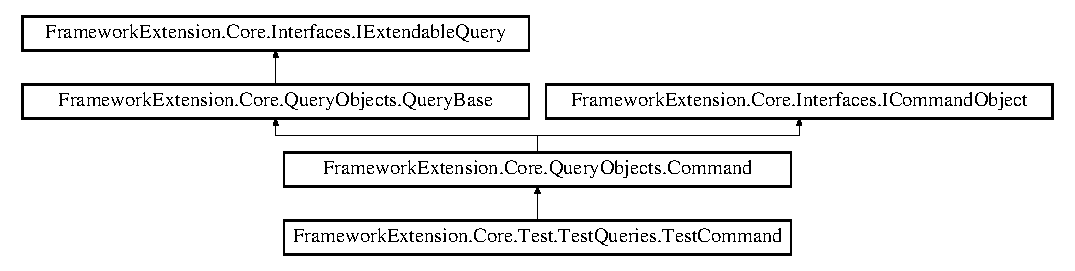
\includegraphics[height=3.200000cm]{class_framework_extension_1_1_core_1_1_query_objects_1_1_command}
\end{center}
\end{figure}
\subsection*{Public Member Functions}
\begin{DoxyCompactItemize}
\item 
\hypertarget{class_framework_extension_1_1_core_1_1_query_objects_1_1_command_afb073bf6749a01552e342163d785d90a}{virtual void {\bfseries Execute} (\hyperlink{interface_framework_extension_1_1_core_1_1_interfaces_1_1_i_data_context}{I\-Data\-Context} context)}\label{class_framework_extension_1_1_core_1_1_query_objects_1_1_command_afb073bf6749a01552e342163d785d90a}

\end{DoxyCompactItemize}
\subsection*{Properties}
\begin{DoxyCompactItemize}
\item 
\hypertarget{class_framework_extension_1_1_core_1_1_query_objects_1_1_command_a65fba609b6fb3a4122f2d79b0188c33a}{Action$<$ \hyperlink{interface_framework_extension_1_1_core_1_1_interfaces_1_1_i_data_context}{I\-Data\-Context} $>$ {\bfseries Context\-Query}\hspace{0.3cm}{\ttfamily  \mbox{[}get, set\mbox{]}}}\label{class_framework_extension_1_1_core_1_1_query_objects_1_1_command_a65fba609b6fb3a4122f2d79b0188c33a}

\end{DoxyCompactItemize}
\subsection*{Additional Inherited Members}


The documentation for this class was generated from the following file\-:\begin{DoxyCompactItemize}
\item 
Framework\-Extension.\-Core/\-Query\-Objects/Command.\-cs\end{DoxyCompactItemize}

\hypertarget{class_framework_extension_1_1_entity_framework_1_1_tests_1_1_unit_tests_1_1_commit_events_mock_context}{\section{Framework\-Extension.\-Entity\-Framework.\-Tests.\-Unit\-Tests.\-Commit\-Events\-Mock\-Context Class Reference}
\label{class_framework_extension_1_1_entity_framework_1_1_tests_1_1_unit_tests_1_1_commit_events_mock_context}\index{Framework\-Extension.\-Entity\-Framework.\-Tests.\-Unit\-Tests.\-Commit\-Events\-Mock\-Context@{Framework\-Extension.\-Entity\-Framework.\-Tests.\-Unit\-Tests.\-Commit\-Events\-Mock\-Context}}
}
Inheritance diagram for Framework\-Extension.\-Entity\-Framework.\-Tests.\-Unit\-Tests.\-Commit\-Events\-Mock\-Context\-:\begin{figure}[H]
\begin{center}
\leavevmode
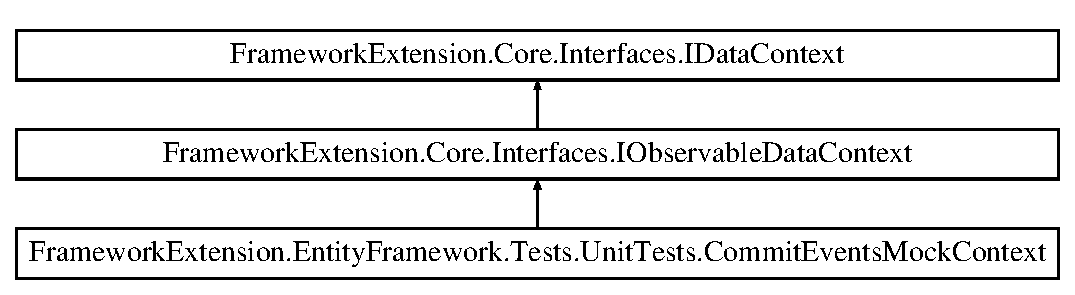
\includegraphics[height=3.000000cm]{class_framework_extension_1_1_entity_framework_1_1_tests_1_1_unit_tests_1_1_commit_events_mock_context}
\end{center}
\end{figure}
\subsection*{Public Member Functions}
\begin{DoxyCompactItemize}
\item 
\hypertarget{class_framework_extension_1_1_entity_framework_1_1_tests_1_1_unit_tests_1_1_commit_events_mock_context_ad82d7b3128c3ebe211590cd135624215}{void {\bfseries Dispose} ()}\label{class_framework_extension_1_1_entity_framework_1_1_tests_1_1_unit_tests_1_1_commit_events_mock_context_ad82d7b3128c3ebe211590cd135624215}

\item 
I\-Queryable$<$ T $>$ \hyperlink{class_framework_extension_1_1_entity_framework_1_1_tests_1_1_unit_tests_1_1_commit_events_mock_context_a1d47f5a08a631c9cb42df64ed2f607c8}{As\-Queryable$<$ T $>$} ()
\begin{DoxyCompactList}\small\item\em This gives a mockable wrapper around the normal Set
\begin{DoxyTemplParams}{Template Parameters}
{\em T} & \\
\hline
\end{DoxyTemplParams}
method that allows for testablity \end{DoxyCompactList}\item 
T \hyperlink{class_framework_extension_1_1_entity_framework_1_1_tests_1_1_unit_tests_1_1_commit_events_mock_context_aa849c2f2553f381457c5003406c5d963}{Add$<$ T $>$} (T item)
\begin{DoxyCompactList}\small\item\em Adds the provided instance of 
\begin{DoxyTemplParams}{Template Parameters}
{\em T} & \\
\hline
\end{DoxyTemplParams}
to the data context \end{DoxyCompactList}\item 
T \hyperlink{class_framework_extension_1_1_entity_framework_1_1_tests_1_1_unit_tests_1_1_commit_events_mock_context_a82ddc0eccd022f543467c4cc4e53db9b}{Remove$<$ T $>$} (T item)
\begin{DoxyCompactList}\small\item\em Removes the provided instance of 
\begin{DoxyTemplParams}{Template Parameters}
{\em T} & \\
\hline
\end{DoxyTemplParams}
from the data context \end{DoxyCompactList}\item 
T \hyperlink{class_framework_extension_1_1_entity_framework_1_1_tests_1_1_unit_tests_1_1_commit_events_mock_context_a0aa0024cf61064e9051e8d722de73a0d}{Update$<$ T $>$} (T item)
\begin{DoxyCompactList}\small\item\em Updates the provided instance of 
\begin{DoxyTemplParams}{Template Parameters}
{\em T} & \\
\hline
\end{DoxyTemplParams}
in the data context \end{DoxyCompactList}\item 
T \hyperlink{class_framework_extension_1_1_entity_framework_1_1_tests_1_1_unit_tests_1_1_commit_events_mock_context_a72aa5f2c99575ef7cce06d776fbb961d}{Attach$<$ T $>$} (T item)
\begin{DoxyCompactList}\small\item\em Attaches the provided instance of 
\begin{DoxyTemplParams}{Template Parameters}
{\em T} & \\
\hline
\end{DoxyTemplParams}
to the data context \end{DoxyCompactList}\item 
T \hyperlink{class_framework_extension_1_1_entity_framework_1_1_tests_1_1_unit_tests_1_1_commit_events_mock_context_a423a62019fb58dfba4170ecd39e4ccfa}{Detach$<$ T $>$} (T item)
\begin{DoxyCompactList}\small\item\em Detaches the provided instance of 
\begin{DoxyTemplParams}{Template Parameters}
{\em T} & \\
\hline
\end{DoxyTemplParams}
from the data context \end{DoxyCompactList}\item 
T \hyperlink{class_framework_extension_1_1_entity_framework_1_1_tests_1_1_unit_tests_1_1_commit_events_mock_context_a50db55322f05c529687fd244b57cdcb9}{Reload$<$ T $>$} (T item)
\begin{DoxyCompactList}\small\item\em Reloads the provided instance of 
\begin{DoxyTemplParams}{Template Parameters}
{\em T} & \\
\hline
\end{DoxyTemplParams}
from the database \end{DoxyCompactList}\item 
void \hyperlink{class_framework_extension_1_1_entity_framework_1_1_tests_1_1_unit_tests_1_1_commit_events_mock_context_a0f247fc4a425272b9d8383cf4896c57c}{Reload$<$ T $>$} ()
\begin{DoxyCompactList}\small\item\em Reloads all tracked objects of the type 
\begin{DoxyTemplParams}{Template Parameters}
{\em T} & \\
\hline
\end{DoxyTemplParams}
\end{DoxyCompactList}\item 
int \hyperlink{class_framework_extension_1_1_entity_framework_1_1_tests_1_1_unit_tests_1_1_commit_events_mock_context_ace62a54842544297557b5ce7a089eb06}{Commit} ()
\begin{DoxyCompactList}\small\item\em Commits all currently tracked entity changes \end{DoxyCompactList}\item 
I\-Enumerable$<$ T $>$ \hyperlink{class_framework_extension_1_1_entity_framework_1_1_tests_1_1_unit_tests_1_1_commit_events_mock_context_a2fd113b93107d60e3ee6832f83741470}{Execute\-Sql\-Query$<$ T $>$} (string sql, params Db\-Parameter\mbox{[}$\,$\mbox{]} db\-Params)
\begin{DoxyCompactList}\small\item\em Executes a S\-Q\-L command and tries to map the returned datasets into an I\-Enumerable
\begin{DoxyTemplParams}{Template Parameters}
{\em T} & \\
\hline
\end{DoxyTemplParams}
The results should have the same column names as the Entity Type has properties \end{DoxyCompactList}\item 
int \hyperlink{class_framework_extension_1_1_entity_framework_1_1_tests_1_1_unit_tests_1_1_commit_events_mock_context_a32fbc6ee30ba43a4348efe2c01d8e20e}{Execute\-Sql\-Command} (string sql, params Db\-Parameter\mbox{[}$\,$\mbox{]} db\-Params)
\begin{DoxyCompactList}\small\item\em Executes a S\-Q\-L command and returns the standard int return from the query \end{DoxyCompactList}\item 
int \hyperlink{class_framework_extension_1_1_entity_framework_1_1_tests_1_1_unit_tests_1_1_commit_events_mock_context_a5fd5f0739acab5d130069397812906ab}{Execute\-Function} (string procedure\-Name, params Object\-Parameter\mbox{[}$\,$\mbox{]} db\-Params)
\begin{DoxyCompactList}\small\item\em \end{DoxyCompactList}\end{DoxyCompactItemize}
\subsection*{Properties}
\begin{DoxyCompactItemize}
\item 
\hypertarget{class_framework_extension_1_1_entity_framework_1_1_tests_1_1_unit_tests_1_1_commit_events_mock_context_a8032ba032da585a733c0e712a0d20e7f}{\hyperlink{interface_framework_extension_1_1_core_1_1_interfaces_1_1_i_event_manager}{I\-Event\-Manager} {\bfseries Event\-Manager}\hspace{0.3cm}{\ttfamily  \mbox{[}get, set\mbox{]}}}\label{class_framework_extension_1_1_entity_framework_1_1_tests_1_1_unit_tests_1_1_commit_events_mock_context_a8032ba032da585a733c0e712a0d20e7f}

\end{DoxyCompactItemize}
\subsection*{Events}
\begin{DoxyCompactItemize}
\item 
\hypertarget{class_framework_extension_1_1_entity_framework_1_1_tests_1_1_unit_tests_1_1_commit_events_mock_context_adc76bca5884d6f003bd23a3da86c4437}{Event\-Handler$<$ \hyperlink{class_framework_extension_1_1_core_1_1_interceptors_1_1_events_1_1_pre_save_event_args}{Pre\-Save\-Event\-Args} $>$ {\bfseries Pre\-Save}}\label{class_framework_extension_1_1_entity_framework_1_1_tests_1_1_unit_tests_1_1_commit_events_mock_context_adc76bca5884d6f003bd23a3da86c4437}

\item 
\hypertarget{class_framework_extension_1_1_entity_framework_1_1_tests_1_1_unit_tests_1_1_commit_events_mock_context_a4db9f067aafe420bdf38f9de6077142d}{Event\-Handler$<$ \hyperlink{class_framework_extension_1_1_core_1_1_interceptors_1_1_events_1_1_post_save_event_args}{Post\-Save\-Event\-Args} $>$ {\bfseries Post\-Save}}\label{class_framework_extension_1_1_entity_framework_1_1_tests_1_1_unit_tests_1_1_commit_events_mock_context_a4db9f067aafe420bdf38f9de6077142d}

\end{DoxyCompactItemize}


\subsection{Member Function Documentation}
\hypertarget{class_framework_extension_1_1_entity_framework_1_1_tests_1_1_unit_tests_1_1_commit_events_mock_context_aa849c2f2553f381457c5003406c5d963}{\index{Framework\-Extension\-::\-Entity\-Framework\-::\-Tests\-::\-Unit\-Tests\-::\-Commit\-Events\-Mock\-Context@{Framework\-Extension\-::\-Entity\-Framework\-::\-Tests\-::\-Unit\-Tests\-::\-Commit\-Events\-Mock\-Context}!Add$<$ T $>$@{Add$<$ T $>$}}
\index{Add$<$ T $>$@{Add$<$ T $>$}!FrameworkExtension::EntityFramework::Tests::UnitTests::CommitEventsMockContext@{Framework\-Extension\-::\-Entity\-Framework\-::\-Tests\-::\-Unit\-Tests\-::\-Commit\-Events\-Mock\-Context}}
\subsubsection[{Add$<$ T $>$}]{\setlength{\rightskip}{0pt plus 5cm}T Framework\-Extension.\-Entity\-Framework.\-Tests.\-Unit\-Tests.\-Commit\-Events\-Mock\-Context.\-Add$<$ T $>$ (
\begin{DoxyParamCaption}
\item[{T}]{item}
\end{DoxyParamCaption}
)\hspace{0.3cm}{\ttfamily [inline]}}}\label{class_framework_extension_1_1_entity_framework_1_1_tests_1_1_unit_tests_1_1_commit_events_mock_context_aa849c2f2553f381457c5003406c5d963}


Adds the provided instance of 
\begin{DoxyTemplParams}{Template Parameters}
{\em T} & \\
\hline
\end{DoxyTemplParams}
to the data context 


\begin{DoxyTemplParams}{Template Parameters}
{\em T} & The Entity Type being added\\
\hline
\end{DoxyTemplParams}

\begin{DoxyParams}{Parameters}
{\em item} & The 
\begin{DoxyTemplParams}{Template Parameters}
{\em T} & \\
\hline
\end{DoxyTemplParams}
you want to add\\
\hline
\end{DoxyParams}
\begin{DoxyReturn}{Returns}
The 
\begin{DoxyTemplParams}{Template Parameters}
{\em T} & \\
\hline
\end{DoxyTemplParams}
you added
\end{DoxyReturn}


Implements \hyperlink{interface_framework_extension_1_1_core_1_1_interfaces_1_1_i_data_context_a0c8685ab4b1c99f897eba29fba179896}{Framework\-Extension.\-Core.\-Interfaces.\-I\-Data\-Context}.

\begin{Desc}
\item[Type Constraints]\begin{description}
\item[{\em T} : {\em class}]\end{description}
\end{Desc}
\hypertarget{class_framework_extension_1_1_entity_framework_1_1_tests_1_1_unit_tests_1_1_commit_events_mock_context_a1d47f5a08a631c9cb42df64ed2f607c8}{\index{Framework\-Extension\-::\-Entity\-Framework\-::\-Tests\-::\-Unit\-Tests\-::\-Commit\-Events\-Mock\-Context@{Framework\-Extension\-::\-Entity\-Framework\-::\-Tests\-::\-Unit\-Tests\-::\-Commit\-Events\-Mock\-Context}!As\-Queryable$<$ T $>$@{As\-Queryable$<$ T $>$}}
\index{As\-Queryable$<$ T $>$@{As\-Queryable$<$ T $>$}!FrameworkExtension::EntityFramework::Tests::UnitTests::CommitEventsMockContext@{Framework\-Extension\-::\-Entity\-Framework\-::\-Tests\-::\-Unit\-Tests\-::\-Commit\-Events\-Mock\-Context}}
\subsubsection[{As\-Queryable$<$ T $>$}]{\setlength{\rightskip}{0pt plus 5cm}I\-Queryable$<$T$>$ Framework\-Extension.\-Entity\-Framework.\-Tests.\-Unit\-Tests.\-Commit\-Events\-Mock\-Context.\-As\-Queryable$<$ T $>$ (
\begin{DoxyParamCaption}
{}
\end{DoxyParamCaption}
)\hspace{0.3cm}{\ttfamily [inline]}}}\label{class_framework_extension_1_1_entity_framework_1_1_tests_1_1_unit_tests_1_1_commit_events_mock_context_a1d47f5a08a631c9cb42df64ed2f607c8}


This gives a mockable wrapper around the normal Set
\begin{DoxyTemplParams}{Template Parameters}
{\em T} & \\
\hline
\end{DoxyTemplParams}
method that allows for testablity 


\begin{DoxyTemplParams}{Template Parameters}
{\em T} & The Entity being queried\\
\hline
\end{DoxyTemplParams}
\begin{DoxyReturn}{Returns}
I\-Queryable
\begin{DoxyTemplParams}{Template Parameters}
{\em T} & \\
\hline
\end{DoxyTemplParams}

\end{DoxyReturn}


Implements \hyperlink{interface_framework_extension_1_1_core_1_1_interfaces_1_1_i_data_context_a815dee1d6eb11910fc12250752b654b7}{Framework\-Extension.\-Core.\-Interfaces.\-I\-Data\-Context}.

\begin{Desc}
\item[Type Constraints]\begin{description}
\item[{\em T} : {\em class}]\end{description}
\end{Desc}
\hypertarget{class_framework_extension_1_1_entity_framework_1_1_tests_1_1_unit_tests_1_1_commit_events_mock_context_a72aa5f2c99575ef7cce06d776fbb961d}{\index{Framework\-Extension\-::\-Entity\-Framework\-::\-Tests\-::\-Unit\-Tests\-::\-Commit\-Events\-Mock\-Context@{Framework\-Extension\-::\-Entity\-Framework\-::\-Tests\-::\-Unit\-Tests\-::\-Commit\-Events\-Mock\-Context}!Attach$<$ T $>$@{Attach$<$ T $>$}}
\index{Attach$<$ T $>$@{Attach$<$ T $>$}!FrameworkExtension::EntityFramework::Tests::UnitTests::CommitEventsMockContext@{Framework\-Extension\-::\-Entity\-Framework\-::\-Tests\-::\-Unit\-Tests\-::\-Commit\-Events\-Mock\-Context}}
\subsubsection[{Attach$<$ T $>$}]{\setlength{\rightskip}{0pt plus 5cm}T Framework\-Extension.\-Entity\-Framework.\-Tests.\-Unit\-Tests.\-Commit\-Events\-Mock\-Context.\-Attach$<$ T $>$ (
\begin{DoxyParamCaption}
\item[{T}]{item}
\end{DoxyParamCaption}
)\hspace{0.3cm}{\ttfamily [inline]}}}\label{class_framework_extension_1_1_entity_framework_1_1_tests_1_1_unit_tests_1_1_commit_events_mock_context_a72aa5f2c99575ef7cce06d776fbb961d}


Attaches the provided instance of 
\begin{DoxyTemplParams}{Template Parameters}
{\em T} & \\
\hline
\end{DoxyTemplParams}
to the data context 


\begin{DoxyTemplParams}{Template Parameters}
{\em T} & The Entity Type being attached\\
\hline
\end{DoxyTemplParams}

\begin{DoxyParams}{Parameters}
{\em item} & The 
\begin{DoxyTemplParams}{Template Parameters}
{\em T} & \\
\hline
\end{DoxyTemplParams}
you want to attach\\
\hline
\end{DoxyParams}
\begin{DoxyReturn}{Returns}
The 
\begin{DoxyTemplParams}{Template Parameters}
{\em T} & \\
\hline
\end{DoxyTemplParams}
you attached
\end{DoxyReturn}


Implements \hyperlink{interface_framework_extension_1_1_core_1_1_interfaces_1_1_i_data_context_afb8535c9b4c824dcc7787ee1c8f987e8}{Framework\-Extension.\-Core.\-Interfaces.\-I\-Data\-Context}.

\begin{Desc}
\item[Type Constraints]\begin{description}
\item[{\em T} : {\em class}]\end{description}
\end{Desc}
\hypertarget{class_framework_extension_1_1_entity_framework_1_1_tests_1_1_unit_tests_1_1_commit_events_mock_context_ace62a54842544297557b5ce7a089eb06}{\index{Framework\-Extension\-::\-Entity\-Framework\-::\-Tests\-::\-Unit\-Tests\-::\-Commit\-Events\-Mock\-Context@{Framework\-Extension\-::\-Entity\-Framework\-::\-Tests\-::\-Unit\-Tests\-::\-Commit\-Events\-Mock\-Context}!Commit@{Commit}}
\index{Commit@{Commit}!FrameworkExtension::EntityFramework::Tests::UnitTests::CommitEventsMockContext@{Framework\-Extension\-::\-Entity\-Framework\-::\-Tests\-::\-Unit\-Tests\-::\-Commit\-Events\-Mock\-Context}}
\subsubsection[{Commit}]{\setlength{\rightskip}{0pt plus 5cm}int Framework\-Extension.\-Entity\-Framework.\-Tests.\-Unit\-Tests.\-Commit\-Events\-Mock\-Context.\-Commit (
\begin{DoxyParamCaption}
{}
\end{DoxyParamCaption}
)\hspace{0.3cm}{\ttfamily [inline]}}}\label{class_framework_extension_1_1_entity_framework_1_1_tests_1_1_unit_tests_1_1_commit_events_mock_context_ace62a54842544297557b5ce7a089eb06}


Commits all currently tracked entity changes 

\begin{DoxyReturn}{Returns}
the number of rows affected
\end{DoxyReturn}


Implements \hyperlink{interface_framework_extension_1_1_core_1_1_interfaces_1_1_i_data_context_a50f3923131c6dbd2d5b057558327d9b2}{Framework\-Extension.\-Core.\-Interfaces.\-I\-Data\-Context}.

\hypertarget{class_framework_extension_1_1_entity_framework_1_1_tests_1_1_unit_tests_1_1_commit_events_mock_context_a423a62019fb58dfba4170ecd39e4ccfa}{\index{Framework\-Extension\-::\-Entity\-Framework\-::\-Tests\-::\-Unit\-Tests\-::\-Commit\-Events\-Mock\-Context@{Framework\-Extension\-::\-Entity\-Framework\-::\-Tests\-::\-Unit\-Tests\-::\-Commit\-Events\-Mock\-Context}!Detach$<$ T $>$@{Detach$<$ T $>$}}
\index{Detach$<$ T $>$@{Detach$<$ T $>$}!FrameworkExtension::EntityFramework::Tests::UnitTests::CommitEventsMockContext@{Framework\-Extension\-::\-Entity\-Framework\-::\-Tests\-::\-Unit\-Tests\-::\-Commit\-Events\-Mock\-Context}}
\subsubsection[{Detach$<$ T $>$}]{\setlength{\rightskip}{0pt plus 5cm}T Framework\-Extension.\-Entity\-Framework.\-Tests.\-Unit\-Tests.\-Commit\-Events\-Mock\-Context.\-Detach$<$ T $>$ (
\begin{DoxyParamCaption}
\item[{T}]{item}
\end{DoxyParamCaption}
)\hspace{0.3cm}{\ttfamily [inline]}}}\label{class_framework_extension_1_1_entity_framework_1_1_tests_1_1_unit_tests_1_1_commit_events_mock_context_a423a62019fb58dfba4170ecd39e4ccfa}


Detaches the provided instance of 
\begin{DoxyTemplParams}{Template Parameters}
{\em T} & \\
\hline
\end{DoxyTemplParams}
from the data context 


\begin{DoxyTemplParams}{Template Parameters}
{\em T} & The Entity Type being detached\\
\hline
\end{DoxyTemplParams}

\begin{DoxyParams}{Parameters}
{\em item} & The 
\begin{DoxyTemplParams}{Template Parameters}
{\em T} & \\
\hline
\end{DoxyTemplParams}
you want to detach\\
\hline
\end{DoxyParams}
\begin{DoxyReturn}{Returns}
The 
\begin{DoxyTemplParams}{Template Parameters}
{\em T} & \\
\hline
\end{DoxyTemplParams}
you detached
\end{DoxyReturn}


Implements \hyperlink{interface_framework_extension_1_1_core_1_1_interfaces_1_1_i_data_context_a26dc0d9a711b046a891f4796774a868f}{Framework\-Extension.\-Core.\-Interfaces.\-I\-Data\-Context}.

\begin{Desc}
\item[Type Constraints]\begin{description}
\item[{\em T} : {\em class}]\end{description}
\end{Desc}
\hypertarget{class_framework_extension_1_1_entity_framework_1_1_tests_1_1_unit_tests_1_1_commit_events_mock_context_a5fd5f0739acab5d130069397812906ab}{\index{Framework\-Extension\-::\-Entity\-Framework\-::\-Tests\-::\-Unit\-Tests\-::\-Commit\-Events\-Mock\-Context@{Framework\-Extension\-::\-Entity\-Framework\-::\-Tests\-::\-Unit\-Tests\-::\-Commit\-Events\-Mock\-Context}!Execute\-Function@{Execute\-Function}}
\index{Execute\-Function@{Execute\-Function}!FrameworkExtension::EntityFramework::Tests::UnitTests::CommitEventsMockContext@{Framework\-Extension\-::\-Entity\-Framework\-::\-Tests\-::\-Unit\-Tests\-::\-Commit\-Events\-Mock\-Context}}
\subsubsection[{Execute\-Function}]{\setlength{\rightskip}{0pt plus 5cm}int Framework\-Extension.\-Entity\-Framework.\-Tests.\-Unit\-Tests.\-Commit\-Events\-Mock\-Context.\-Execute\-Function (
\begin{DoxyParamCaption}
\item[{string}]{procedure\-Name, }
\item[{params Object\-Parameter\mbox{[}$\,$\mbox{]}}]{db\-Params}
\end{DoxyParamCaption}
)\hspace{0.3cm}{\ttfamily [inline]}}}\label{class_framework_extension_1_1_entity_framework_1_1_tests_1_1_unit_tests_1_1_commit_events_mock_context_a5fd5f0739acab5d130069397812906ab}





\begin{DoxyParams}{Parameters}
{\em procedure\-Name} & \\
\hline
{\em db\-Params} & \\
\hline
\end{DoxyParams}
\begin{DoxyReturn}{Returns}

\end{DoxyReturn}


Implements \hyperlink{interface_framework_extension_1_1_core_1_1_interfaces_1_1_i_data_context_a4fd23b695358dfafb3a2547fc78ce0ef}{Framework\-Extension.\-Core.\-Interfaces.\-I\-Data\-Context}.

\hypertarget{class_framework_extension_1_1_entity_framework_1_1_tests_1_1_unit_tests_1_1_commit_events_mock_context_a32fbc6ee30ba43a4348efe2c01d8e20e}{\index{Framework\-Extension\-::\-Entity\-Framework\-::\-Tests\-::\-Unit\-Tests\-::\-Commit\-Events\-Mock\-Context@{Framework\-Extension\-::\-Entity\-Framework\-::\-Tests\-::\-Unit\-Tests\-::\-Commit\-Events\-Mock\-Context}!Execute\-Sql\-Command@{Execute\-Sql\-Command}}
\index{Execute\-Sql\-Command@{Execute\-Sql\-Command}!FrameworkExtension::EntityFramework::Tests::UnitTests::CommitEventsMockContext@{Framework\-Extension\-::\-Entity\-Framework\-::\-Tests\-::\-Unit\-Tests\-::\-Commit\-Events\-Mock\-Context}}
\subsubsection[{Execute\-Sql\-Command}]{\setlength{\rightskip}{0pt plus 5cm}int Framework\-Extension.\-Entity\-Framework.\-Tests.\-Unit\-Tests.\-Commit\-Events\-Mock\-Context.\-Execute\-Sql\-Command (
\begin{DoxyParamCaption}
\item[{string}]{sql, }
\item[{params Db\-Parameter\mbox{[}$\,$\mbox{]}}]{db\-Params}
\end{DoxyParamCaption}
)\hspace{0.3cm}{\ttfamily [inline]}}}\label{class_framework_extension_1_1_entity_framework_1_1_tests_1_1_unit_tests_1_1_commit_events_mock_context_a32fbc6ee30ba43a4348efe2c01d8e20e}


Executes a S\-Q\-L command and returns the standard int return from the query 


\begin{DoxyParams}{Parameters}
{\em sql} & The Sql Statement\\
\hline
{\em db\-Params} & A List of Database Parameters for the Query\\
\hline
\end{DoxyParams}
\begin{DoxyReturn}{Returns}
The rows affected
\end{DoxyReturn}


Implements \hyperlink{interface_framework_extension_1_1_core_1_1_interfaces_1_1_i_data_context_a1deee0a581593b6ae859816fb9f243e2}{Framework\-Extension.\-Core.\-Interfaces.\-I\-Data\-Context}.

\hypertarget{class_framework_extension_1_1_entity_framework_1_1_tests_1_1_unit_tests_1_1_commit_events_mock_context_a2fd113b93107d60e3ee6832f83741470}{\index{Framework\-Extension\-::\-Entity\-Framework\-::\-Tests\-::\-Unit\-Tests\-::\-Commit\-Events\-Mock\-Context@{Framework\-Extension\-::\-Entity\-Framework\-::\-Tests\-::\-Unit\-Tests\-::\-Commit\-Events\-Mock\-Context}!Execute\-Sql\-Query$<$ T $>$@{Execute\-Sql\-Query$<$ T $>$}}
\index{Execute\-Sql\-Query$<$ T $>$@{Execute\-Sql\-Query$<$ T $>$}!FrameworkExtension::EntityFramework::Tests::UnitTests::CommitEventsMockContext@{Framework\-Extension\-::\-Entity\-Framework\-::\-Tests\-::\-Unit\-Tests\-::\-Commit\-Events\-Mock\-Context}}
\subsubsection[{Execute\-Sql\-Query$<$ T $>$}]{\setlength{\rightskip}{0pt plus 5cm}I\-Enumerable$<$T$>$ Framework\-Extension.\-Entity\-Framework.\-Tests.\-Unit\-Tests.\-Commit\-Events\-Mock\-Context.\-Execute\-Sql\-Query$<$ T $>$ (
\begin{DoxyParamCaption}
\item[{string}]{sql, }
\item[{params Db\-Parameter\mbox{[}$\,$\mbox{]}}]{db\-Params}
\end{DoxyParamCaption}
)\hspace{0.3cm}{\ttfamily [inline]}}}\label{class_framework_extension_1_1_entity_framework_1_1_tests_1_1_unit_tests_1_1_commit_events_mock_context_a2fd113b93107d60e3ee6832f83741470}


Executes a S\-Q\-L command and tries to map the returned datasets into an I\-Enumerable
\begin{DoxyTemplParams}{Template Parameters}
{\em T} & \\
\hline
\end{DoxyTemplParams}
The results should have the same column names as the Entity Type has properties 


\begin{DoxyTemplParams}{Template Parameters}
{\em T} & The Entity Type that the return should be mapped to\\
\hline
\end{DoxyTemplParams}

\begin{DoxyParams}{Parameters}
{\em sql} & The Sql Statement\\
\hline
{\em db\-Params} & A List of Database Parameters for the Query\\
\hline
\end{DoxyParams}
\begin{DoxyReturn}{Returns}
An I\-Enumerable
\begin{DoxyTemplParams}{Template Parameters}
{\em T} & \\
\hline
\end{DoxyTemplParams}
from the query return
\end{DoxyReturn}


Implements \hyperlink{interface_framework_extension_1_1_core_1_1_interfaces_1_1_i_data_context_ab2932a3d1a47a5efe2e26083724ed5a0}{Framework\-Extension.\-Core.\-Interfaces.\-I\-Data\-Context}.

\hypertarget{class_framework_extension_1_1_entity_framework_1_1_tests_1_1_unit_tests_1_1_commit_events_mock_context_a50db55322f05c529687fd244b57cdcb9}{\index{Framework\-Extension\-::\-Entity\-Framework\-::\-Tests\-::\-Unit\-Tests\-::\-Commit\-Events\-Mock\-Context@{Framework\-Extension\-::\-Entity\-Framework\-::\-Tests\-::\-Unit\-Tests\-::\-Commit\-Events\-Mock\-Context}!Reload$<$ T $>$@{Reload$<$ T $>$}}
\index{Reload$<$ T $>$@{Reload$<$ T $>$}!FrameworkExtension::EntityFramework::Tests::UnitTests::CommitEventsMockContext@{Framework\-Extension\-::\-Entity\-Framework\-::\-Tests\-::\-Unit\-Tests\-::\-Commit\-Events\-Mock\-Context}}
\subsubsection[{Reload$<$ T $>$}]{\setlength{\rightskip}{0pt plus 5cm}T Framework\-Extension.\-Entity\-Framework.\-Tests.\-Unit\-Tests.\-Commit\-Events\-Mock\-Context.\-Reload$<$ T $>$ (
\begin{DoxyParamCaption}
\item[{T}]{item}
\end{DoxyParamCaption}
)\hspace{0.3cm}{\ttfamily [inline]}}}\label{class_framework_extension_1_1_entity_framework_1_1_tests_1_1_unit_tests_1_1_commit_events_mock_context_a50db55322f05c529687fd244b57cdcb9}


Reloads the provided instance of 
\begin{DoxyTemplParams}{Template Parameters}
{\em T} & \\
\hline
\end{DoxyTemplParams}
from the database 


\begin{DoxyTemplParams}{Template Parameters}
{\em T} & The Entity Type being reloaded\\
\hline
\end{DoxyTemplParams}

\begin{DoxyParams}{Parameters}
{\em item} & The 
\begin{DoxyTemplParams}{Template Parameters}
{\em T} & \\
\hline
\end{DoxyTemplParams}
you want to reload\\
\hline
\end{DoxyParams}
\begin{DoxyReturn}{Returns}
The 
\begin{DoxyTemplParams}{Template Parameters}
{\em T} & \\
\hline
\end{DoxyTemplParams}
you reloaded
\end{DoxyReturn}


Implements \hyperlink{interface_framework_extension_1_1_core_1_1_interfaces_1_1_i_data_context_a0440afc85c29fbe35b62685a08fb2313}{Framework\-Extension.\-Core.\-Interfaces.\-I\-Data\-Context}.

\begin{Desc}
\item[Type Constraints]\begin{description}
\item[{\em T} : {\em class}]\end{description}
\end{Desc}
\hypertarget{class_framework_extension_1_1_entity_framework_1_1_tests_1_1_unit_tests_1_1_commit_events_mock_context_a0f247fc4a425272b9d8383cf4896c57c}{\index{Framework\-Extension\-::\-Entity\-Framework\-::\-Tests\-::\-Unit\-Tests\-::\-Commit\-Events\-Mock\-Context@{Framework\-Extension\-::\-Entity\-Framework\-::\-Tests\-::\-Unit\-Tests\-::\-Commit\-Events\-Mock\-Context}!Reload$<$ T $>$@{Reload$<$ T $>$}}
\index{Reload$<$ T $>$@{Reload$<$ T $>$}!FrameworkExtension::EntityFramework::Tests::UnitTests::CommitEventsMockContext@{Framework\-Extension\-::\-Entity\-Framework\-::\-Tests\-::\-Unit\-Tests\-::\-Commit\-Events\-Mock\-Context}}
\subsubsection[{Reload$<$ T $>$}]{\setlength{\rightskip}{0pt plus 5cm}void Framework\-Extension.\-Entity\-Framework.\-Tests.\-Unit\-Tests.\-Commit\-Events\-Mock\-Context.\-Reload$<$ T $>$ (
\begin{DoxyParamCaption}
{}
\end{DoxyParamCaption}
)\hspace{0.3cm}{\ttfamily [inline]}}}\label{class_framework_extension_1_1_entity_framework_1_1_tests_1_1_unit_tests_1_1_commit_events_mock_context_a0f247fc4a425272b9d8383cf4896c57c}


Reloads all tracked objects of the type 
\begin{DoxyTemplParams}{Template Parameters}
{\em T} & \\
\hline
\end{DoxyTemplParams}



\begin{DoxyTemplParams}{Template Parameters}
{\em T} & The type of objects to reload\\
\hline
\end{DoxyTemplParams}


Implements \hyperlink{interface_framework_extension_1_1_core_1_1_interfaces_1_1_i_data_context_a0085fcdb37363f377d7ae84522e53a5b}{Framework\-Extension.\-Core.\-Interfaces.\-I\-Data\-Context}.

\begin{Desc}
\item[Type Constraints]\begin{description}
\item[{\em T} : {\em class}]\end{description}
\end{Desc}
\hypertarget{class_framework_extension_1_1_entity_framework_1_1_tests_1_1_unit_tests_1_1_commit_events_mock_context_a82ddc0eccd022f543467c4cc4e53db9b}{\index{Framework\-Extension\-::\-Entity\-Framework\-::\-Tests\-::\-Unit\-Tests\-::\-Commit\-Events\-Mock\-Context@{Framework\-Extension\-::\-Entity\-Framework\-::\-Tests\-::\-Unit\-Tests\-::\-Commit\-Events\-Mock\-Context}!Remove$<$ T $>$@{Remove$<$ T $>$}}
\index{Remove$<$ T $>$@{Remove$<$ T $>$}!FrameworkExtension::EntityFramework::Tests::UnitTests::CommitEventsMockContext@{Framework\-Extension\-::\-Entity\-Framework\-::\-Tests\-::\-Unit\-Tests\-::\-Commit\-Events\-Mock\-Context}}
\subsubsection[{Remove$<$ T $>$}]{\setlength{\rightskip}{0pt plus 5cm}T Framework\-Extension.\-Entity\-Framework.\-Tests.\-Unit\-Tests.\-Commit\-Events\-Mock\-Context.\-Remove$<$ T $>$ (
\begin{DoxyParamCaption}
\item[{T}]{item}
\end{DoxyParamCaption}
)\hspace{0.3cm}{\ttfamily [inline]}}}\label{class_framework_extension_1_1_entity_framework_1_1_tests_1_1_unit_tests_1_1_commit_events_mock_context_a82ddc0eccd022f543467c4cc4e53db9b}


Removes the provided instance of 
\begin{DoxyTemplParams}{Template Parameters}
{\em T} & \\
\hline
\end{DoxyTemplParams}
from the data context 


\begin{DoxyTemplParams}{Template Parameters}
{\em T} & The Entity Type being removed\\
\hline
\end{DoxyTemplParams}

\begin{DoxyParams}{Parameters}
{\em item} & The 
\begin{DoxyTemplParams}{Template Parameters}
{\em T} & \\
\hline
\end{DoxyTemplParams}
you want to remove\\
\hline
\end{DoxyParams}
\begin{DoxyReturn}{Returns}
The 
\begin{DoxyTemplParams}{Template Parameters}
{\em T} & \\
\hline
\end{DoxyTemplParams}
you removed
\end{DoxyReturn}


Implements \hyperlink{interface_framework_extension_1_1_core_1_1_interfaces_1_1_i_data_context_a713205a05d584b6d47325434e6723564}{Framework\-Extension.\-Core.\-Interfaces.\-I\-Data\-Context}.

\begin{Desc}
\item[Type Constraints]\begin{description}
\item[{\em T} : {\em class}]\end{description}
\end{Desc}
\hypertarget{class_framework_extension_1_1_entity_framework_1_1_tests_1_1_unit_tests_1_1_commit_events_mock_context_a0aa0024cf61064e9051e8d722de73a0d}{\index{Framework\-Extension\-::\-Entity\-Framework\-::\-Tests\-::\-Unit\-Tests\-::\-Commit\-Events\-Mock\-Context@{Framework\-Extension\-::\-Entity\-Framework\-::\-Tests\-::\-Unit\-Tests\-::\-Commit\-Events\-Mock\-Context}!Update$<$ T $>$@{Update$<$ T $>$}}
\index{Update$<$ T $>$@{Update$<$ T $>$}!FrameworkExtension::EntityFramework::Tests::UnitTests::CommitEventsMockContext@{Framework\-Extension\-::\-Entity\-Framework\-::\-Tests\-::\-Unit\-Tests\-::\-Commit\-Events\-Mock\-Context}}
\subsubsection[{Update$<$ T $>$}]{\setlength{\rightskip}{0pt plus 5cm}T Framework\-Extension.\-Entity\-Framework.\-Tests.\-Unit\-Tests.\-Commit\-Events\-Mock\-Context.\-Update$<$ T $>$ (
\begin{DoxyParamCaption}
\item[{T}]{item}
\end{DoxyParamCaption}
)\hspace{0.3cm}{\ttfamily [inline]}}}\label{class_framework_extension_1_1_entity_framework_1_1_tests_1_1_unit_tests_1_1_commit_events_mock_context_a0aa0024cf61064e9051e8d722de73a0d}


Updates the provided instance of 
\begin{DoxyTemplParams}{Template Parameters}
{\em T} & \\
\hline
\end{DoxyTemplParams}
in the data context 


\begin{DoxyTemplParams}{Template Parameters}
{\em T} & The Entity Type being updated\\
\hline
\end{DoxyTemplParams}

\begin{DoxyParams}{Parameters}
{\em item} & The 
\begin{DoxyTemplParams}{Template Parameters}
{\em T} & \\
\hline
\end{DoxyTemplParams}
you want to update\\
\hline
\end{DoxyParams}
\begin{DoxyReturn}{Returns}
The 
\begin{DoxyTemplParams}{Template Parameters}
{\em T} & \\
\hline
\end{DoxyTemplParams}
you updated
\end{DoxyReturn}


Implements \hyperlink{interface_framework_extension_1_1_core_1_1_interfaces_1_1_i_data_context_a1297c0d6e59ec05855d8e25a72f49fdd}{Framework\-Extension.\-Core.\-Interfaces.\-I\-Data\-Context}.

\begin{Desc}
\item[Type Constraints]\begin{description}
\item[{\em T} : {\em class}]\end{description}
\end{Desc}


The documentation for this class was generated from the following file\-:\begin{DoxyCompactItemize}
\item 
Framework\-Extension.\-Entity\-Framework.\-Tests/\-Unit\-Tests/Given\-\_\-\-An\-\_\-\-Event\-\_\-\-Extendable\-\_\-\-Context.\-cs\end{DoxyCompactItemize}

\hypertarget{class_framework_extension_1_1_core_1_1_services_1_1_default_user_name_service}{\section{Framework\-Extension.\-Core.\-Services.\-Default\-User\-Name\-Service Class Reference}
\label{class_framework_extension_1_1_core_1_1_services_1_1_default_user_name_service}\index{Framework\-Extension.\-Core.\-Services.\-Default\-User\-Name\-Service@{Framework\-Extension.\-Core.\-Services.\-Default\-User\-Name\-Service}}
}
Inheritance diagram for Framework\-Extension.\-Core.\-Services.\-Default\-User\-Name\-Service\-:\begin{figure}[H]
\begin{center}
\leavevmode
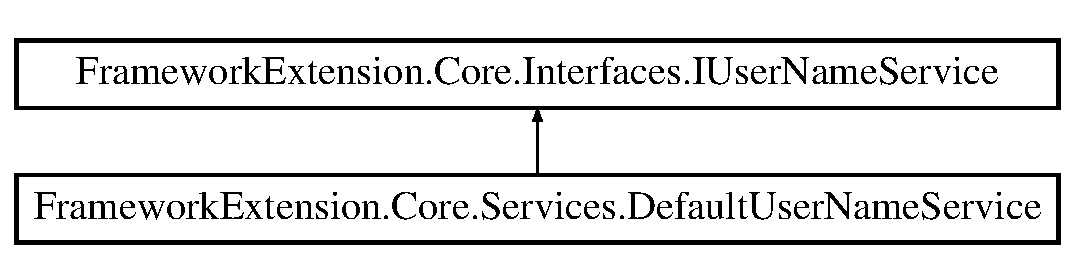
\includegraphics[height=2.000000cm]{class_framework_extension_1_1_core_1_1_services_1_1_default_user_name_service}
\end{center}
\end{figure}
\subsection*{Public Member Functions}
\begin{DoxyCompactItemize}
\item 
\hypertarget{class_framework_extension_1_1_core_1_1_services_1_1_default_user_name_service_aaa3a0df3d14c34e0ac74f341f817fe0a}{string {\bfseries Get\-Current\-User\-Name} ()}\label{class_framework_extension_1_1_core_1_1_services_1_1_default_user_name_service_aaa3a0df3d14c34e0ac74f341f817fe0a}

\end{DoxyCompactItemize}


The documentation for this class was generated from the following file\-:\begin{DoxyCompactItemize}
\item 
Framework\-Extension.\-Core/\-Services/Default\-User\-Name\-Service.\-cs\end{DoxyCompactItemize}

\hypertarget{class_framework_extension_1_1_entity_framework_1_1_tests_1_1_unit_tests_1_1_e_f_failure_context}{\section{Framework\-Extension.\-Entity\-Framework.\-Tests.\-Unit\-Tests.\-E\-F\-Failure\-Context Class Reference}
\label{class_framework_extension_1_1_entity_framework_1_1_tests_1_1_unit_tests_1_1_e_f_failure_context}\index{Framework\-Extension.\-Entity\-Framework.\-Tests.\-Unit\-Tests.\-E\-F\-Failure\-Context@{Framework\-Extension.\-Entity\-Framework.\-Tests.\-Unit\-Tests.\-E\-F\-Failure\-Context}}
}
Inheritance diagram for Framework\-Extension.\-Entity\-Framework.\-Tests.\-Unit\-Tests.\-E\-F\-Failure\-Context\-:\begin{figure}[H]
\begin{center}
\leavevmode
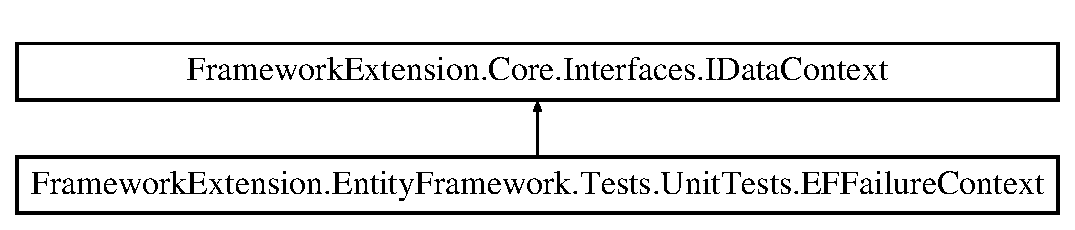
\includegraphics[height=2.000000cm]{class_framework_extension_1_1_entity_framework_1_1_tests_1_1_unit_tests_1_1_e_f_failure_context}
\end{center}
\end{figure}
\subsection*{Public Member Functions}
\begin{DoxyCompactItemize}
\item 
I\-Queryable$<$ T $>$ \hyperlink{class_framework_extension_1_1_entity_framework_1_1_tests_1_1_unit_tests_1_1_e_f_failure_context_a6991c5a792c54f0a1a695907e52ba685}{As\-Queryable$<$ T $>$} ()
\begin{DoxyCompactList}\small\item\em This gives a mockable wrapper around the normal Set
\begin{DoxyTemplParams}{Template Parameters}
{\em T} & \\
\hline
\end{DoxyTemplParams}
method that allows for testablity \end{DoxyCompactList}\item 
T \hyperlink{class_framework_extension_1_1_entity_framework_1_1_tests_1_1_unit_tests_1_1_e_f_failure_context_a8e82869480647106cd2369cbbbe9ca49}{Add$<$ T $>$} (T item)
\begin{DoxyCompactList}\small\item\em Adds the provided instance of 
\begin{DoxyTemplParams}{Template Parameters}
{\em T} & \\
\hline
\end{DoxyTemplParams}
to the data context \end{DoxyCompactList}\item 
\hypertarget{class_framework_extension_1_1_entity_framework_1_1_tests_1_1_unit_tests_1_1_e_f_failure_context_a989a7cf4b7800016d3e9413ad5cd788a}{T {\bfseries Add$<$ T $>$} (T item, bool change\-State)}\label{class_framework_extension_1_1_entity_framework_1_1_tests_1_1_unit_tests_1_1_e_f_failure_context_a989a7cf4b7800016d3e9413ad5cd788a}

\item 
T \hyperlink{class_framework_extension_1_1_entity_framework_1_1_tests_1_1_unit_tests_1_1_e_f_failure_context_a2a577ce94c9ea67d1f3d255c3f4aa9d8}{Remove$<$ T $>$} (T item)
\begin{DoxyCompactList}\small\item\em Removes the provided instance of 
\begin{DoxyTemplParams}{Template Parameters}
{\em T} & \\
\hline
\end{DoxyTemplParams}
from the data context \end{DoxyCompactList}\item 
T \hyperlink{class_framework_extension_1_1_entity_framework_1_1_tests_1_1_unit_tests_1_1_e_f_failure_context_a784fd14d08113d264b8bf40d57a54b34}{Update$<$ T $>$} (T item)
\begin{DoxyCompactList}\small\item\em Updates the provided instance of 
\begin{DoxyTemplParams}{Template Parameters}
{\em T} & \\
\hline
\end{DoxyTemplParams}
in the data context \end{DoxyCompactList}\item 
T \hyperlink{class_framework_extension_1_1_entity_framework_1_1_tests_1_1_unit_tests_1_1_e_f_failure_context_a08e5c8cc89f1409bf58fce39d097935c}{Attach$<$ T $>$} (T item)
\begin{DoxyCompactList}\small\item\em Attaches the provided instance of 
\begin{DoxyTemplParams}{Template Parameters}
{\em T} & \\
\hline
\end{DoxyTemplParams}
to the data context \end{DoxyCompactList}\item 
T \hyperlink{class_framework_extension_1_1_entity_framework_1_1_tests_1_1_unit_tests_1_1_e_f_failure_context_aa33403a155b2131363fa93932d4c89f8}{Detach$<$ T $>$} (T item)
\begin{DoxyCompactList}\small\item\em Detaches the provided instance of 
\begin{DoxyTemplParams}{Template Parameters}
{\em T} & \\
\hline
\end{DoxyTemplParams}
from the data context \end{DoxyCompactList}\item 
T \hyperlink{class_framework_extension_1_1_entity_framework_1_1_tests_1_1_unit_tests_1_1_e_f_failure_context_a9ae371619fb677cd081d9540ee0da028}{Reload$<$ T $>$} (T item)
\begin{DoxyCompactList}\small\item\em Reloads the provided instance of 
\begin{DoxyTemplParams}{Template Parameters}
{\em T} & \\
\hline
\end{DoxyTemplParams}
from the database \end{DoxyCompactList}\item 
void \hyperlink{class_framework_extension_1_1_entity_framework_1_1_tests_1_1_unit_tests_1_1_e_f_failure_context_a8853cd1e280cdd8c1a46589239b1ba12}{Reload$<$ T $>$} ()
\begin{DoxyCompactList}\small\item\em Reloads all tracked objects of the type 
\begin{DoxyTemplParams}{Template Parameters}
{\em T} & \\
\hline
\end{DoxyTemplParams}
\end{DoxyCompactList}\item 
int \hyperlink{class_framework_extension_1_1_entity_framework_1_1_tests_1_1_unit_tests_1_1_e_f_failure_context_a470c419e85cd5e9f262219c00f7f50c6}{Commit} ()
\begin{DoxyCompactList}\small\item\em Commits all currently tracked entity changes \end{DoxyCompactList}\item 
int \hyperlink{class_framework_extension_1_1_entity_framework_1_1_tests_1_1_unit_tests_1_1_e_f_failure_context_aacb855d688d7782535b817ec31a470d3}{Execute\-Function} (string procedure\-Name, params Object\-Parameter\mbox{[}$\,$\mbox{]} db\-Params)
\begin{DoxyCompactList}\small\item\em \end{DoxyCompactList}\item 
int \hyperlink{class_framework_extension_1_1_entity_framework_1_1_tests_1_1_unit_tests_1_1_e_f_failure_context_a3a9251810905d4fe3a1193ba2d447a86}{Execute\-Sql\-Command} (string sql, params Db\-Parameter\mbox{[}$\,$\mbox{]} db\-Params)
\begin{DoxyCompactList}\small\item\em Executes a S\-Q\-L command and returns the standard int return from the query \end{DoxyCompactList}\item 
I\-Enumerable$<$ T $>$ \hyperlink{class_framework_extension_1_1_entity_framework_1_1_tests_1_1_unit_tests_1_1_e_f_failure_context_ad70050780ddca2e8a5e749a3e0d26a32}{Execute\-Sql\-Query$<$ T $>$} (string sql, params Db\-Parameter\mbox{[}$\,$\mbox{]} db\-Params)
\begin{DoxyCompactList}\small\item\em Executes a S\-Q\-L command and tries to map the returned datasets into an I\-Enumerable
\begin{DoxyTemplParams}{Template Parameters}
{\em T} & \\
\hline
\end{DoxyTemplParams}
The results should have the same column names as the Entity Type has properties \end{DoxyCompactList}\item 
\hypertarget{class_framework_extension_1_1_entity_framework_1_1_tests_1_1_unit_tests_1_1_e_f_failure_context_aed3e8575020a1d9a7d9717f6809049de}{void {\bfseries Dispose} ()}\label{class_framework_extension_1_1_entity_framework_1_1_tests_1_1_unit_tests_1_1_e_f_failure_context_aed3e8575020a1d9a7d9717f6809049de}

\end{DoxyCompactItemize}
\subsection*{Properties}
\begin{DoxyCompactItemize}
\item 
\hypertarget{class_framework_extension_1_1_entity_framework_1_1_tests_1_1_unit_tests_1_1_e_f_failure_context_a898f25dd9c01586a0f0bdca7a6b4abed}{\hyperlink{interface_framework_extension_1_1_core_1_1_interfaces_1_1_i_event_manager}{I\-Event\-Manager} {\bfseries Event\-Manager}\hspace{0.3cm}{\ttfamily  \mbox{[}get, set\mbox{]}}}\label{class_framework_extension_1_1_entity_framework_1_1_tests_1_1_unit_tests_1_1_e_f_failure_context_a898f25dd9c01586a0f0bdca7a6b4abed}

\end{DoxyCompactItemize}


\subsection{Member Function Documentation}
\hypertarget{class_framework_extension_1_1_entity_framework_1_1_tests_1_1_unit_tests_1_1_e_f_failure_context_a8e82869480647106cd2369cbbbe9ca49}{\index{Framework\-Extension\-::\-Entity\-Framework\-::\-Tests\-::\-Unit\-Tests\-::\-E\-F\-Failure\-Context@{Framework\-Extension\-::\-Entity\-Framework\-::\-Tests\-::\-Unit\-Tests\-::\-E\-F\-Failure\-Context}!Add$<$ T $>$@{Add$<$ T $>$}}
\index{Add$<$ T $>$@{Add$<$ T $>$}!FrameworkExtension::EntityFramework::Tests::UnitTests::EFFailureContext@{Framework\-Extension\-::\-Entity\-Framework\-::\-Tests\-::\-Unit\-Tests\-::\-E\-F\-Failure\-Context}}
\subsubsection[{Add$<$ T $>$}]{\setlength{\rightskip}{0pt plus 5cm}T Framework\-Extension.\-Entity\-Framework.\-Tests.\-Unit\-Tests.\-E\-F\-Failure\-Context.\-Add$<$ T $>$ (
\begin{DoxyParamCaption}
\item[{T}]{item}
\end{DoxyParamCaption}
)\hspace{0.3cm}{\ttfamily [inline]}}}\label{class_framework_extension_1_1_entity_framework_1_1_tests_1_1_unit_tests_1_1_e_f_failure_context_a8e82869480647106cd2369cbbbe9ca49}


Adds the provided instance of 
\begin{DoxyTemplParams}{Template Parameters}
{\em T} & \\
\hline
\end{DoxyTemplParams}
to the data context 


\begin{DoxyTemplParams}{Template Parameters}
{\em T} & The Entity Type being added\\
\hline
\end{DoxyTemplParams}

\begin{DoxyParams}{Parameters}
{\em item} & The 
\begin{DoxyTemplParams}{Template Parameters}
{\em T} & \\
\hline
\end{DoxyTemplParams}
you want to add\\
\hline
\end{DoxyParams}
\begin{DoxyReturn}{Returns}
The 
\begin{DoxyTemplParams}{Template Parameters}
{\em T} & \\
\hline
\end{DoxyTemplParams}
you added
\end{DoxyReturn}


Implements \hyperlink{interface_framework_extension_1_1_core_1_1_interfaces_1_1_i_data_context_a0c8685ab4b1c99f897eba29fba179896}{Framework\-Extension.\-Core.\-Interfaces.\-I\-Data\-Context}.

\begin{Desc}
\item[Type Constraints]\begin{description}
\item[{\em T} : {\em class}]\end{description}
\end{Desc}
\hypertarget{class_framework_extension_1_1_entity_framework_1_1_tests_1_1_unit_tests_1_1_e_f_failure_context_a6991c5a792c54f0a1a695907e52ba685}{\index{Framework\-Extension\-::\-Entity\-Framework\-::\-Tests\-::\-Unit\-Tests\-::\-E\-F\-Failure\-Context@{Framework\-Extension\-::\-Entity\-Framework\-::\-Tests\-::\-Unit\-Tests\-::\-E\-F\-Failure\-Context}!As\-Queryable$<$ T $>$@{As\-Queryable$<$ T $>$}}
\index{As\-Queryable$<$ T $>$@{As\-Queryable$<$ T $>$}!FrameworkExtension::EntityFramework::Tests::UnitTests::EFFailureContext@{Framework\-Extension\-::\-Entity\-Framework\-::\-Tests\-::\-Unit\-Tests\-::\-E\-F\-Failure\-Context}}
\subsubsection[{As\-Queryable$<$ T $>$}]{\setlength{\rightskip}{0pt plus 5cm}I\-Queryable$<$T$>$ Framework\-Extension.\-Entity\-Framework.\-Tests.\-Unit\-Tests.\-E\-F\-Failure\-Context.\-As\-Queryable$<$ T $>$ (
\begin{DoxyParamCaption}
{}
\end{DoxyParamCaption}
)\hspace{0.3cm}{\ttfamily [inline]}}}\label{class_framework_extension_1_1_entity_framework_1_1_tests_1_1_unit_tests_1_1_e_f_failure_context_a6991c5a792c54f0a1a695907e52ba685}


This gives a mockable wrapper around the normal Set
\begin{DoxyTemplParams}{Template Parameters}
{\em T} & \\
\hline
\end{DoxyTemplParams}
method that allows for testablity 


\begin{DoxyTemplParams}{Template Parameters}
{\em T} & The Entity being queried\\
\hline
\end{DoxyTemplParams}
\begin{DoxyReturn}{Returns}
I\-Queryable
\begin{DoxyTemplParams}{Template Parameters}
{\em T} & \\
\hline
\end{DoxyTemplParams}

\end{DoxyReturn}


Implements \hyperlink{interface_framework_extension_1_1_core_1_1_interfaces_1_1_i_data_context_a815dee1d6eb11910fc12250752b654b7}{Framework\-Extension.\-Core.\-Interfaces.\-I\-Data\-Context}.

\hypertarget{class_framework_extension_1_1_entity_framework_1_1_tests_1_1_unit_tests_1_1_e_f_failure_context_a08e5c8cc89f1409bf58fce39d097935c}{\index{Framework\-Extension\-::\-Entity\-Framework\-::\-Tests\-::\-Unit\-Tests\-::\-E\-F\-Failure\-Context@{Framework\-Extension\-::\-Entity\-Framework\-::\-Tests\-::\-Unit\-Tests\-::\-E\-F\-Failure\-Context}!Attach$<$ T $>$@{Attach$<$ T $>$}}
\index{Attach$<$ T $>$@{Attach$<$ T $>$}!FrameworkExtension::EntityFramework::Tests::UnitTests::EFFailureContext@{Framework\-Extension\-::\-Entity\-Framework\-::\-Tests\-::\-Unit\-Tests\-::\-E\-F\-Failure\-Context}}
\subsubsection[{Attach$<$ T $>$}]{\setlength{\rightskip}{0pt plus 5cm}T Framework\-Extension.\-Entity\-Framework.\-Tests.\-Unit\-Tests.\-E\-F\-Failure\-Context.\-Attach$<$ T $>$ (
\begin{DoxyParamCaption}
\item[{T}]{item}
\end{DoxyParamCaption}
)\hspace{0.3cm}{\ttfamily [inline]}}}\label{class_framework_extension_1_1_entity_framework_1_1_tests_1_1_unit_tests_1_1_e_f_failure_context_a08e5c8cc89f1409bf58fce39d097935c}


Attaches the provided instance of 
\begin{DoxyTemplParams}{Template Parameters}
{\em T} & \\
\hline
\end{DoxyTemplParams}
to the data context 


\begin{DoxyTemplParams}{Template Parameters}
{\em T} & The Entity Type being attached\\
\hline
\end{DoxyTemplParams}

\begin{DoxyParams}{Parameters}
{\em item} & The 
\begin{DoxyTemplParams}{Template Parameters}
{\em T} & \\
\hline
\end{DoxyTemplParams}
you want to attach\\
\hline
\end{DoxyParams}
\begin{DoxyReturn}{Returns}
The 
\begin{DoxyTemplParams}{Template Parameters}
{\em T} & \\
\hline
\end{DoxyTemplParams}
you attached
\end{DoxyReturn}


Implements \hyperlink{interface_framework_extension_1_1_core_1_1_interfaces_1_1_i_data_context_afb8535c9b4c824dcc7787ee1c8f987e8}{Framework\-Extension.\-Core.\-Interfaces.\-I\-Data\-Context}.

\begin{Desc}
\item[Type Constraints]\begin{description}
\item[{\em T} : {\em class}]\end{description}
\end{Desc}
\hypertarget{class_framework_extension_1_1_entity_framework_1_1_tests_1_1_unit_tests_1_1_e_f_failure_context_a470c419e85cd5e9f262219c00f7f50c6}{\index{Framework\-Extension\-::\-Entity\-Framework\-::\-Tests\-::\-Unit\-Tests\-::\-E\-F\-Failure\-Context@{Framework\-Extension\-::\-Entity\-Framework\-::\-Tests\-::\-Unit\-Tests\-::\-E\-F\-Failure\-Context}!Commit@{Commit}}
\index{Commit@{Commit}!FrameworkExtension::EntityFramework::Tests::UnitTests::EFFailureContext@{Framework\-Extension\-::\-Entity\-Framework\-::\-Tests\-::\-Unit\-Tests\-::\-E\-F\-Failure\-Context}}
\subsubsection[{Commit}]{\setlength{\rightskip}{0pt plus 5cm}int Framework\-Extension.\-Entity\-Framework.\-Tests.\-Unit\-Tests.\-E\-F\-Failure\-Context.\-Commit (
\begin{DoxyParamCaption}
{}
\end{DoxyParamCaption}
)\hspace{0.3cm}{\ttfamily [inline]}}}\label{class_framework_extension_1_1_entity_framework_1_1_tests_1_1_unit_tests_1_1_e_f_failure_context_a470c419e85cd5e9f262219c00f7f50c6}


Commits all currently tracked entity changes 

\begin{DoxyReturn}{Returns}
the number of rows affected
\end{DoxyReturn}


Implements \hyperlink{interface_framework_extension_1_1_core_1_1_interfaces_1_1_i_data_context_a50f3923131c6dbd2d5b057558327d9b2}{Framework\-Extension.\-Core.\-Interfaces.\-I\-Data\-Context}.

\hypertarget{class_framework_extension_1_1_entity_framework_1_1_tests_1_1_unit_tests_1_1_e_f_failure_context_aa33403a155b2131363fa93932d4c89f8}{\index{Framework\-Extension\-::\-Entity\-Framework\-::\-Tests\-::\-Unit\-Tests\-::\-E\-F\-Failure\-Context@{Framework\-Extension\-::\-Entity\-Framework\-::\-Tests\-::\-Unit\-Tests\-::\-E\-F\-Failure\-Context}!Detach$<$ T $>$@{Detach$<$ T $>$}}
\index{Detach$<$ T $>$@{Detach$<$ T $>$}!FrameworkExtension::EntityFramework::Tests::UnitTests::EFFailureContext@{Framework\-Extension\-::\-Entity\-Framework\-::\-Tests\-::\-Unit\-Tests\-::\-E\-F\-Failure\-Context}}
\subsubsection[{Detach$<$ T $>$}]{\setlength{\rightskip}{0pt plus 5cm}T Framework\-Extension.\-Entity\-Framework.\-Tests.\-Unit\-Tests.\-E\-F\-Failure\-Context.\-Detach$<$ T $>$ (
\begin{DoxyParamCaption}
\item[{T}]{item}
\end{DoxyParamCaption}
)\hspace{0.3cm}{\ttfamily [inline]}}}\label{class_framework_extension_1_1_entity_framework_1_1_tests_1_1_unit_tests_1_1_e_f_failure_context_aa33403a155b2131363fa93932d4c89f8}


Detaches the provided instance of 
\begin{DoxyTemplParams}{Template Parameters}
{\em T} & \\
\hline
\end{DoxyTemplParams}
from the data context 


\begin{DoxyTemplParams}{Template Parameters}
{\em T} & The Entity Type being detached\\
\hline
\end{DoxyTemplParams}

\begin{DoxyParams}{Parameters}
{\em item} & The 
\begin{DoxyTemplParams}{Template Parameters}
{\em T} & \\
\hline
\end{DoxyTemplParams}
you want to detach\\
\hline
\end{DoxyParams}
\begin{DoxyReturn}{Returns}
The 
\begin{DoxyTemplParams}{Template Parameters}
{\em T} & \\
\hline
\end{DoxyTemplParams}
you detached
\end{DoxyReturn}


Implements \hyperlink{interface_framework_extension_1_1_core_1_1_interfaces_1_1_i_data_context_a26dc0d9a711b046a891f4796774a868f}{Framework\-Extension.\-Core.\-Interfaces.\-I\-Data\-Context}.

\begin{Desc}
\item[Type Constraints]\begin{description}
\item[{\em T} : {\em class}]\end{description}
\end{Desc}
\hypertarget{class_framework_extension_1_1_entity_framework_1_1_tests_1_1_unit_tests_1_1_e_f_failure_context_aacb855d688d7782535b817ec31a470d3}{\index{Framework\-Extension\-::\-Entity\-Framework\-::\-Tests\-::\-Unit\-Tests\-::\-E\-F\-Failure\-Context@{Framework\-Extension\-::\-Entity\-Framework\-::\-Tests\-::\-Unit\-Tests\-::\-E\-F\-Failure\-Context}!Execute\-Function@{Execute\-Function}}
\index{Execute\-Function@{Execute\-Function}!FrameworkExtension::EntityFramework::Tests::UnitTests::EFFailureContext@{Framework\-Extension\-::\-Entity\-Framework\-::\-Tests\-::\-Unit\-Tests\-::\-E\-F\-Failure\-Context}}
\subsubsection[{Execute\-Function}]{\setlength{\rightskip}{0pt plus 5cm}int Framework\-Extension.\-Entity\-Framework.\-Tests.\-Unit\-Tests.\-E\-F\-Failure\-Context.\-Execute\-Function (
\begin{DoxyParamCaption}
\item[{string}]{procedure\-Name, }
\item[{params Object\-Parameter\mbox{[}$\,$\mbox{]}}]{db\-Params}
\end{DoxyParamCaption}
)\hspace{0.3cm}{\ttfamily [inline]}}}\label{class_framework_extension_1_1_entity_framework_1_1_tests_1_1_unit_tests_1_1_e_f_failure_context_aacb855d688d7782535b817ec31a470d3}





\begin{DoxyParams}{Parameters}
{\em procedure\-Name} & \\
\hline
{\em db\-Params} & \\
\hline
\end{DoxyParams}
\begin{DoxyReturn}{Returns}

\end{DoxyReturn}


Implements \hyperlink{interface_framework_extension_1_1_core_1_1_interfaces_1_1_i_data_context_a4fd23b695358dfafb3a2547fc78ce0ef}{Framework\-Extension.\-Core.\-Interfaces.\-I\-Data\-Context}.

\hypertarget{class_framework_extension_1_1_entity_framework_1_1_tests_1_1_unit_tests_1_1_e_f_failure_context_a3a9251810905d4fe3a1193ba2d447a86}{\index{Framework\-Extension\-::\-Entity\-Framework\-::\-Tests\-::\-Unit\-Tests\-::\-E\-F\-Failure\-Context@{Framework\-Extension\-::\-Entity\-Framework\-::\-Tests\-::\-Unit\-Tests\-::\-E\-F\-Failure\-Context}!Execute\-Sql\-Command@{Execute\-Sql\-Command}}
\index{Execute\-Sql\-Command@{Execute\-Sql\-Command}!FrameworkExtension::EntityFramework::Tests::UnitTests::EFFailureContext@{Framework\-Extension\-::\-Entity\-Framework\-::\-Tests\-::\-Unit\-Tests\-::\-E\-F\-Failure\-Context}}
\subsubsection[{Execute\-Sql\-Command}]{\setlength{\rightskip}{0pt plus 5cm}int Framework\-Extension.\-Entity\-Framework.\-Tests.\-Unit\-Tests.\-E\-F\-Failure\-Context.\-Execute\-Sql\-Command (
\begin{DoxyParamCaption}
\item[{string}]{sql, }
\item[{params Db\-Parameter\mbox{[}$\,$\mbox{]}}]{db\-Params}
\end{DoxyParamCaption}
)\hspace{0.3cm}{\ttfamily [inline]}}}\label{class_framework_extension_1_1_entity_framework_1_1_tests_1_1_unit_tests_1_1_e_f_failure_context_a3a9251810905d4fe3a1193ba2d447a86}


Executes a S\-Q\-L command and returns the standard int return from the query 


\begin{DoxyParams}{Parameters}
{\em sql} & The Sql Statement\\
\hline
{\em db\-Params} & A List of Database Parameters for the Query\\
\hline
\end{DoxyParams}
\begin{DoxyReturn}{Returns}
The rows affected
\end{DoxyReturn}


Implements \hyperlink{interface_framework_extension_1_1_core_1_1_interfaces_1_1_i_data_context_a1deee0a581593b6ae859816fb9f243e2}{Framework\-Extension.\-Core.\-Interfaces.\-I\-Data\-Context}.

\hypertarget{class_framework_extension_1_1_entity_framework_1_1_tests_1_1_unit_tests_1_1_e_f_failure_context_ad70050780ddca2e8a5e749a3e0d26a32}{\index{Framework\-Extension\-::\-Entity\-Framework\-::\-Tests\-::\-Unit\-Tests\-::\-E\-F\-Failure\-Context@{Framework\-Extension\-::\-Entity\-Framework\-::\-Tests\-::\-Unit\-Tests\-::\-E\-F\-Failure\-Context}!Execute\-Sql\-Query$<$ T $>$@{Execute\-Sql\-Query$<$ T $>$}}
\index{Execute\-Sql\-Query$<$ T $>$@{Execute\-Sql\-Query$<$ T $>$}!FrameworkExtension::EntityFramework::Tests::UnitTests::EFFailureContext@{Framework\-Extension\-::\-Entity\-Framework\-::\-Tests\-::\-Unit\-Tests\-::\-E\-F\-Failure\-Context}}
\subsubsection[{Execute\-Sql\-Query$<$ T $>$}]{\setlength{\rightskip}{0pt plus 5cm}I\-Enumerable$<$T$>$ Framework\-Extension.\-Entity\-Framework.\-Tests.\-Unit\-Tests.\-E\-F\-Failure\-Context.\-Execute\-Sql\-Query$<$ T $>$ (
\begin{DoxyParamCaption}
\item[{string}]{sql, }
\item[{params Db\-Parameter\mbox{[}$\,$\mbox{]}}]{db\-Params}
\end{DoxyParamCaption}
)\hspace{0.3cm}{\ttfamily [inline]}}}\label{class_framework_extension_1_1_entity_framework_1_1_tests_1_1_unit_tests_1_1_e_f_failure_context_ad70050780ddca2e8a5e749a3e0d26a32}


Executes a S\-Q\-L command and tries to map the returned datasets into an I\-Enumerable
\begin{DoxyTemplParams}{Template Parameters}
{\em T} & \\
\hline
\end{DoxyTemplParams}
The results should have the same column names as the Entity Type has properties 


\begin{DoxyTemplParams}{Template Parameters}
{\em T} & The Entity Type that the return should be mapped to\\
\hline
\end{DoxyTemplParams}

\begin{DoxyParams}{Parameters}
{\em sql} & The Sql Statement\\
\hline
{\em db\-Params} & A List of Database Parameters for the Query\\
\hline
\end{DoxyParams}
\begin{DoxyReturn}{Returns}
An I\-Enumerable
\begin{DoxyTemplParams}{Template Parameters}
{\em T} & \\
\hline
\end{DoxyTemplParams}
from the query return
\end{DoxyReturn}


Implements \hyperlink{interface_framework_extension_1_1_core_1_1_interfaces_1_1_i_data_context_ab2932a3d1a47a5efe2e26083724ed5a0}{Framework\-Extension.\-Core.\-Interfaces.\-I\-Data\-Context}.

\hypertarget{class_framework_extension_1_1_entity_framework_1_1_tests_1_1_unit_tests_1_1_e_f_failure_context_a9ae371619fb677cd081d9540ee0da028}{\index{Framework\-Extension\-::\-Entity\-Framework\-::\-Tests\-::\-Unit\-Tests\-::\-E\-F\-Failure\-Context@{Framework\-Extension\-::\-Entity\-Framework\-::\-Tests\-::\-Unit\-Tests\-::\-E\-F\-Failure\-Context}!Reload$<$ T $>$@{Reload$<$ T $>$}}
\index{Reload$<$ T $>$@{Reload$<$ T $>$}!FrameworkExtension::EntityFramework::Tests::UnitTests::EFFailureContext@{Framework\-Extension\-::\-Entity\-Framework\-::\-Tests\-::\-Unit\-Tests\-::\-E\-F\-Failure\-Context}}
\subsubsection[{Reload$<$ T $>$}]{\setlength{\rightskip}{0pt plus 5cm}T Framework\-Extension.\-Entity\-Framework.\-Tests.\-Unit\-Tests.\-E\-F\-Failure\-Context.\-Reload$<$ T $>$ (
\begin{DoxyParamCaption}
\item[{T}]{item}
\end{DoxyParamCaption}
)\hspace{0.3cm}{\ttfamily [inline]}}}\label{class_framework_extension_1_1_entity_framework_1_1_tests_1_1_unit_tests_1_1_e_f_failure_context_a9ae371619fb677cd081d9540ee0da028}


Reloads the provided instance of 
\begin{DoxyTemplParams}{Template Parameters}
{\em T} & \\
\hline
\end{DoxyTemplParams}
from the database 


\begin{DoxyTemplParams}{Template Parameters}
{\em T} & The Entity Type being reloaded\\
\hline
\end{DoxyTemplParams}

\begin{DoxyParams}{Parameters}
{\em item} & The 
\begin{DoxyTemplParams}{Template Parameters}
{\em T} & \\
\hline
\end{DoxyTemplParams}
you want to reload\\
\hline
\end{DoxyParams}
\begin{DoxyReturn}{Returns}
The 
\begin{DoxyTemplParams}{Template Parameters}
{\em T} & \\
\hline
\end{DoxyTemplParams}
you reloaded
\end{DoxyReturn}


Implements \hyperlink{interface_framework_extension_1_1_core_1_1_interfaces_1_1_i_data_context_a0440afc85c29fbe35b62685a08fb2313}{Framework\-Extension.\-Core.\-Interfaces.\-I\-Data\-Context}.

\begin{Desc}
\item[Type Constraints]\begin{description}
\item[{\em T} : {\em class}]\end{description}
\end{Desc}
\hypertarget{class_framework_extension_1_1_entity_framework_1_1_tests_1_1_unit_tests_1_1_e_f_failure_context_a8853cd1e280cdd8c1a46589239b1ba12}{\index{Framework\-Extension\-::\-Entity\-Framework\-::\-Tests\-::\-Unit\-Tests\-::\-E\-F\-Failure\-Context@{Framework\-Extension\-::\-Entity\-Framework\-::\-Tests\-::\-Unit\-Tests\-::\-E\-F\-Failure\-Context}!Reload$<$ T $>$@{Reload$<$ T $>$}}
\index{Reload$<$ T $>$@{Reload$<$ T $>$}!FrameworkExtension::EntityFramework::Tests::UnitTests::EFFailureContext@{Framework\-Extension\-::\-Entity\-Framework\-::\-Tests\-::\-Unit\-Tests\-::\-E\-F\-Failure\-Context}}
\subsubsection[{Reload$<$ T $>$}]{\setlength{\rightskip}{0pt plus 5cm}void Framework\-Extension.\-Entity\-Framework.\-Tests.\-Unit\-Tests.\-E\-F\-Failure\-Context.\-Reload$<$ T $>$ (
\begin{DoxyParamCaption}
{}
\end{DoxyParamCaption}
)\hspace{0.3cm}{\ttfamily [inline]}}}\label{class_framework_extension_1_1_entity_framework_1_1_tests_1_1_unit_tests_1_1_e_f_failure_context_a8853cd1e280cdd8c1a46589239b1ba12}


Reloads all tracked objects of the type 
\begin{DoxyTemplParams}{Template Parameters}
{\em T} & \\
\hline
\end{DoxyTemplParams}



\begin{DoxyTemplParams}{Template Parameters}
{\em T} & The type of objects to reload\\
\hline
\end{DoxyTemplParams}


Implements \hyperlink{interface_framework_extension_1_1_core_1_1_interfaces_1_1_i_data_context_a0085fcdb37363f377d7ae84522e53a5b}{Framework\-Extension.\-Core.\-Interfaces.\-I\-Data\-Context}.

\begin{Desc}
\item[Type Constraints]\begin{description}
\item[{\em T} : {\em class}]\end{description}
\end{Desc}
\hypertarget{class_framework_extension_1_1_entity_framework_1_1_tests_1_1_unit_tests_1_1_e_f_failure_context_a2a577ce94c9ea67d1f3d255c3f4aa9d8}{\index{Framework\-Extension\-::\-Entity\-Framework\-::\-Tests\-::\-Unit\-Tests\-::\-E\-F\-Failure\-Context@{Framework\-Extension\-::\-Entity\-Framework\-::\-Tests\-::\-Unit\-Tests\-::\-E\-F\-Failure\-Context}!Remove$<$ T $>$@{Remove$<$ T $>$}}
\index{Remove$<$ T $>$@{Remove$<$ T $>$}!FrameworkExtension::EntityFramework::Tests::UnitTests::EFFailureContext@{Framework\-Extension\-::\-Entity\-Framework\-::\-Tests\-::\-Unit\-Tests\-::\-E\-F\-Failure\-Context}}
\subsubsection[{Remove$<$ T $>$}]{\setlength{\rightskip}{0pt plus 5cm}T Framework\-Extension.\-Entity\-Framework.\-Tests.\-Unit\-Tests.\-E\-F\-Failure\-Context.\-Remove$<$ T $>$ (
\begin{DoxyParamCaption}
\item[{T}]{item}
\end{DoxyParamCaption}
)\hspace{0.3cm}{\ttfamily [inline]}}}\label{class_framework_extension_1_1_entity_framework_1_1_tests_1_1_unit_tests_1_1_e_f_failure_context_a2a577ce94c9ea67d1f3d255c3f4aa9d8}


Removes the provided instance of 
\begin{DoxyTemplParams}{Template Parameters}
{\em T} & \\
\hline
\end{DoxyTemplParams}
from the data context 


\begin{DoxyTemplParams}{Template Parameters}
{\em T} & The Entity Type being removed\\
\hline
\end{DoxyTemplParams}

\begin{DoxyParams}{Parameters}
{\em item} & The 
\begin{DoxyTemplParams}{Template Parameters}
{\em T} & \\
\hline
\end{DoxyTemplParams}
you want to remove\\
\hline
\end{DoxyParams}
\begin{DoxyReturn}{Returns}
The 
\begin{DoxyTemplParams}{Template Parameters}
{\em T} & \\
\hline
\end{DoxyTemplParams}
you removed
\end{DoxyReturn}


Implements \hyperlink{interface_framework_extension_1_1_core_1_1_interfaces_1_1_i_data_context_a713205a05d584b6d47325434e6723564}{Framework\-Extension.\-Core.\-Interfaces.\-I\-Data\-Context}.

\begin{Desc}
\item[Type Constraints]\begin{description}
\item[{\em T} : {\em class}]\end{description}
\end{Desc}
\hypertarget{class_framework_extension_1_1_entity_framework_1_1_tests_1_1_unit_tests_1_1_e_f_failure_context_a784fd14d08113d264b8bf40d57a54b34}{\index{Framework\-Extension\-::\-Entity\-Framework\-::\-Tests\-::\-Unit\-Tests\-::\-E\-F\-Failure\-Context@{Framework\-Extension\-::\-Entity\-Framework\-::\-Tests\-::\-Unit\-Tests\-::\-E\-F\-Failure\-Context}!Update$<$ T $>$@{Update$<$ T $>$}}
\index{Update$<$ T $>$@{Update$<$ T $>$}!FrameworkExtension::EntityFramework::Tests::UnitTests::EFFailureContext@{Framework\-Extension\-::\-Entity\-Framework\-::\-Tests\-::\-Unit\-Tests\-::\-E\-F\-Failure\-Context}}
\subsubsection[{Update$<$ T $>$}]{\setlength{\rightskip}{0pt plus 5cm}T Framework\-Extension.\-Entity\-Framework.\-Tests.\-Unit\-Tests.\-E\-F\-Failure\-Context.\-Update$<$ T $>$ (
\begin{DoxyParamCaption}
\item[{T}]{item}
\end{DoxyParamCaption}
)\hspace{0.3cm}{\ttfamily [inline]}}}\label{class_framework_extension_1_1_entity_framework_1_1_tests_1_1_unit_tests_1_1_e_f_failure_context_a784fd14d08113d264b8bf40d57a54b34}


Updates the provided instance of 
\begin{DoxyTemplParams}{Template Parameters}
{\em T} & \\
\hline
\end{DoxyTemplParams}
in the data context 


\begin{DoxyTemplParams}{Template Parameters}
{\em T} & The Entity Type being updated\\
\hline
\end{DoxyTemplParams}

\begin{DoxyParams}{Parameters}
{\em item} & The 
\begin{DoxyTemplParams}{Template Parameters}
{\em T} & \\
\hline
\end{DoxyTemplParams}
you want to update\\
\hline
\end{DoxyParams}
\begin{DoxyReturn}{Returns}
The 
\begin{DoxyTemplParams}{Template Parameters}
{\em T} & \\
\hline
\end{DoxyTemplParams}
you updated
\end{DoxyReturn}


Implements \hyperlink{interface_framework_extension_1_1_core_1_1_interfaces_1_1_i_data_context_a1297c0d6e59ec05855d8e25a72f49fdd}{Framework\-Extension.\-Core.\-Interfaces.\-I\-Data\-Context}.

\begin{Desc}
\item[Type Constraints]\begin{description}
\item[{\em T} : {\em class}]\end{description}
\end{Desc}


The documentation for this class was generated from the following file\-:\begin{DoxyCompactItemize}
\item 
Framework\-Extension.\-Entity\-Framework.\-Tests/\-Unit\-Tests/E\-F\-Failure\-Context.\-cs\end{DoxyCompactItemize}

\hypertarget{class_framework_extension_1_1_entity_framework_1_1_interceptors_1_1_entity_framework_auditable_interceptor}{\section{Framework\-Extension.\-Entity\-Framework.\-Interceptors.\-Entity\-Framework\-Auditable\-Interceptor Class Reference}
\label{class_framework_extension_1_1_entity_framework_1_1_interceptors_1_1_entity_framework_auditable_interceptor}\index{Framework\-Extension.\-Entity\-Framework.\-Interceptors.\-Entity\-Framework\-Auditable\-Interceptor@{Framework\-Extension.\-Entity\-Framework.\-Interceptors.\-Entity\-Framework\-Auditable\-Interceptor}}
}
Inheritance diagram for Framework\-Extension.\-Entity\-Framework.\-Interceptors.\-Entity\-Framework\-Auditable\-Interceptor\-:\begin{figure}[H]
\begin{center}
\leavevmode
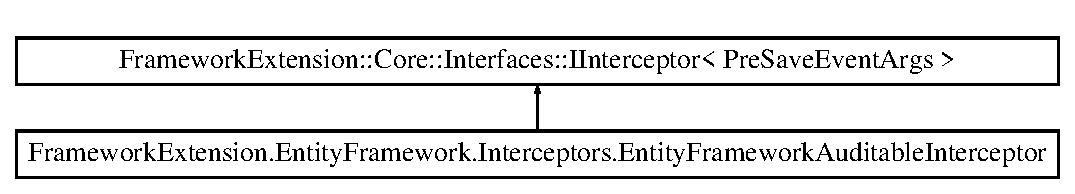
\includegraphics[height=2.000000cm]{class_framework_extension_1_1_entity_framework_1_1_interceptors_1_1_entity_framework_auditable_interceptor}
\end{center}
\end{figure}
\subsection*{Public Member Functions}
\begin{DoxyCompactItemize}
\item 
\hypertarget{class_framework_extension_1_1_entity_framework_1_1_interceptors_1_1_entity_framework_auditable_interceptor_a575bdb30c81c12e567676d17d170aff2}{{\bfseries Entity\-Framework\-Auditable\-Interceptor} (\hyperlink{interface_framework_extension_1_1_core_1_1_interfaces_1_1_i_user_name_service}{I\-User\-Name\-Service} user\-Name\-Service, int priority=0)}\label{class_framework_extension_1_1_entity_framework_1_1_interceptors_1_1_entity_framework_auditable_interceptor_a575bdb30c81c12e567676d17d170aff2}

\item 
\hypertarget{class_framework_extension_1_1_entity_framework_1_1_interceptors_1_1_entity_framework_auditable_interceptor_a55dd1ba5a9ca146e3fd0e8219f69f48b}{\hyperlink{struct_framework_extension_1_1_core_1_1_interceptors_1_1_interceptor_result}{Interceptor\-Result} {\bfseries Execute} (\hyperlink{interface_framework_extension_1_1_core_1_1_interfaces_1_1_i_data_context}{I\-Data\-Context} context, \hyperlink{class_framework_extension_1_1_core_1_1_interceptors_1_1_events_1_1_pre_save_event_args}{Pre\-Save\-Event\-Args} event\-Args)}\label{class_framework_extension_1_1_entity_framework_1_1_interceptors_1_1_entity_framework_auditable_interceptor_a55dd1ba5a9ca146e3fd0e8219f69f48b}

\end{DoxyCompactItemize}
\subsection*{Properties}
\begin{DoxyCompactItemize}
\item 
\hypertarget{class_framework_extension_1_1_entity_framework_1_1_interceptors_1_1_entity_framework_auditable_interceptor_a5d109fa0dc420c3e236dd98ddcb6eade}{int {\bfseries Priority}\hspace{0.3cm}{\ttfamily  \mbox{[}get, set\mbox{]}}}\label{class_framework_extension_1_1_entity_framework_1_1_interceptors_1_1_entity_framework_auditable_interceptor_a5d109fa0dc420c3e236dd98ddcb6eade}

\end{DoxyCompactItemize}


The documentation for this class was generated from the following file\-:\begin{DoxyCompactItemize}
\item 
Framework\-Extension.\-Entity\-Framework/\-Interceptors/Entity\-Framework\-Auditable\-Interceptor.\-cs\end{DoxyCompactItemize}

\hypertarget{class_framework_extension_1_1_entity_framework_1_1_contexts_1_1_entity_framework_context}{\section{Framework\-Extension.\-Entity\-Framework.\-Contexts.\-Entity\-Framework\-Context Class Reference}
\label{class_framework_extension_1_1_entity_framework_1_1_contexts_1_1_entity_framework_context}\index{Framework\-Extension.\-Entity\-Framework.\-Contexts.\-Entity\-Framework\-Context@{Framework\-Extension.\-Entity\-Framework.\-Contexts.\-Entity\-Framework\-Context}}
}
Inheritance diagram for Framework\-Extension.\-Entity\-Framework.\-Contexts.\-Entity\-Framework\-Context\-:\begin{figure}[H]
\begin{center}
\leavevmode
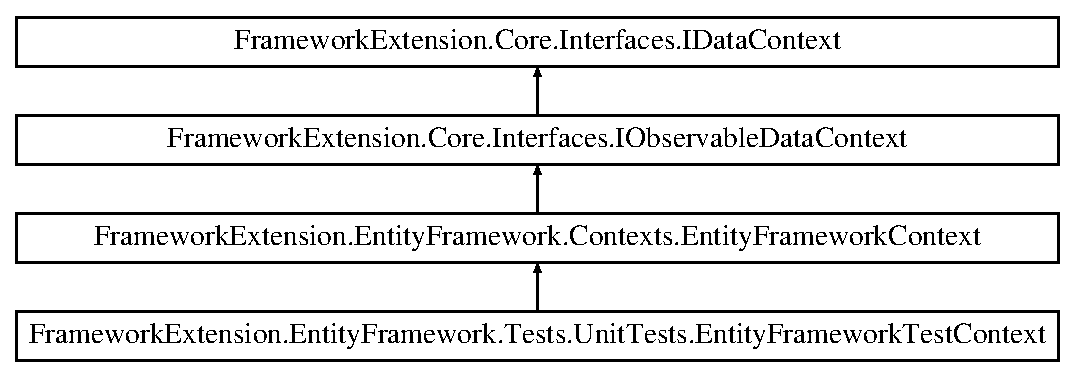
\includegraphics[height=4.000000cm]{class_framework_extension_1_1_entity_framework_1_1_contexts_1_1_entity_framework_context}
\end{center}
\end{figure}
\subsection*{Public Member Functions}
\begin{DoxyCompactItemize}
\item 
\hyperlink{class_framework_extension_1_1_entity_framework_1_1_contexts_1_1_entity_framework_context_a37fb0de705ec1e6ca5f7cbe39c5e47ae}{Entity\-Framework\-Context} (string connection\-String, \hyperlink{interface_framework_extension_1_1_entity_framework_1_1_mappings_1_1_i_mapping_configuration}{I\-Mapping\-Configuration} configuration)
\begin{DoxyCompactList}\small\item\em Constructs a context \end{DoxyCompactList}\item 
I\-Queryable$<$ T $>$ \hyperlink{class_framework_extension_1_1_entity_framework_1_1_contexts_1_1_entity_framework_context_a56d3f290277a320f9fb8a3045c4d530c}{As\-Queryable$<$ T $>$} ()
\begin{DoxyCompactList}\small\item\em This gives a mockable wrapper around the normal Set
\begin{DoxyTemplParams}{Template Parameters}
{\em T} & \\
\hline
\end{DoxyTemplParams}
method that allows for testablity \end{DoxyCompactList}\item 
T \hyperlink{class_framework_extension_1_1_entity_framework_1_1_contexts_1_1_entity_framework_context_ae3053c572db5a34802107c6734e8d758}{Add$<$ T $>$} (T item)
\begin{DoxyCompactList}\small\item\em Adds the provided instance of 
\begin{DoxyTemplParams}{Template Parameters}
{\em T} & \\
\hline
\end{DoxyTemplParams}
to the data context \end{DoxyCompactList}\item 
T \hyperlink{class_framework_extension_1_1_entity_framework_1_1_contexts_1_1_entity_framework_context_ac56f15278782a2978a3d5f368156ef8d}{Remove$<$ T $>$} (T item)
\begin{DoxyCompactList}\small\item\em Removes the provided instance of 
\begin{DoxyTemplParams}{Template Parameters}
{\em T} & \\
\hline
\end{DoxyTemplParams}
from the data context \end{DoxyCompactList}\item 
T \hyperlink{class_framework_extension_1_1_entity_framework_1_1_contexts_1_1_entity_framework_context_a02b78487a49ea0d42aeee143bff5c0bc}{Update$<$ T $>$} (T item)
\begin{DoxyCompactList}\small\item\em Updates the provided instance of 
\begin{DoxyTemplParams}{Template Parameters}
{\em T} & \\
\hline
\end{DoxyTemplParams}
in the data context \end{DoxyCompactList}\item 
T \hyperlink{class_framework_extension_1_1_entity_framework_1_1_contexts_1_1_entity_framework_context_a44750d8bf54f6d8ba284d46544c221fb}{Attach$<$ T $>$} (T item)
\begin{DoxyCompactList}\small\item\em Attaches the provided instance of 
\begin{DoxyTemplParams}{Template Parameters}
{\em T} & \\
\hline
\end{DoxyTemplParams}
to the data context \end{DoxyCompactList}\item 
T \hyperlink{class_framework_extension_1_1_entity_framework_1_1_contexts_1_1_entity_framework_context_a057c2858fd25f18db69fc85b86eb2019}{Detach$<$ T $>$} (T item)
\begin{DoxyCompactList}\small\item\em Detaches the provided instance of 
\begin{DoxyTemplParams}{Template Parameters}
{\em T} & \\
\hline
\end{DoxyTemplParams}
from the data context \end{DoxyCompactList}\item 
T \hyperlink{class_framework_extension_1_1_entity_framework_1_1_contexts_1_1_entity_framework_context_ac8c74190bfe433a8eae0658616bad089}{Reload$<$ T $>$} (T item)
\begin{DoxyCompactList}\small\item\em Reloads the provided instance of 
\begin{DoxyTemplParams}{Template Parameters}
{\em T} & \\
\hline
\end{DoxyTemplParams}
from the database \end{DoxyCompactList}\item 
void \hyperlink{class_framework_extension_1_1_entity_framework_1_1_contexts_1_1_entity_framework_context_a87a885ec11e09fce2f7f220e6c98f994}{Reload$<$ T $>$} ()
\begin{DoxyCompactList}\small\item\em Reloads all tracked objects of the type 
\begin{DoxyTemplParams}{Template Parameters}
{\em T} & \\
\hline
\end{DoxyTemplParams}
\end{DoxyCompactList}\item 
int \hyperlink{class_framework_extension_1_1_entity_framework_1_1_contexts_1_1_entity_framework_context_ac7563d83d7010a5f8da3168cf43fe5be}{Commit} ()
\begin{DoxyCompactList}\small\item\em Commits all currently tracked entity changes \end{DoxyCompactList}\item 
I\-Enumerable$<$ T $>$ \hyperlink{class_framework_extension_1_1_entity_framework_1_1_contexts_1_1_entity_framework_context_a307fa6de8b9356b1d0addf4e2fd35b17}{Execute\-Sql\-Query$<$ T $>$} (string sql, params Db\-Parameter\mbox{[}$\,$\mbox{]} db\-Params)
\begin{DoxyCompactList}\small\item\em Executes a S\-Q\-L command and tries to map the returned datasets into an I\-Enumerable
\begin{DoxyTemplParams}{Template Parameters}
{\em T} & \\
\hline
\end{DoxyTemplParams}
The results should have the same column names as the Entity Type has properties \end{DoxyCompactList}\item 
int \hyperlink{class_framework_extension_1_1_entity_framework_1_1_contexts_1_1_entity_framework_context_a322a4ad4a30196edfd0f7aed48b9bf73}{Execute\-Sql\-Command} (string sql, params Db\-Parameter\mbox{[}$\,$\mbox{]} db\-Params)
\begin{DoxyCompactList}\small\item\em Executes a S\-Q\-L command and returns the standard int return from the query \end{DoxyCompactList}\item 
int \hyperlink{class_framework_extension_1_1_entity_framework_1_1_contexts_1_1_entity_framework_context_a8348891845aee02967ca1d4c1c1ec786}{Execute\-Function} (string procedure\-Name, params Object\-Parameter\mbox{[}$\,$\mbox{]} db\-Params)
\begin{DoxyCompactList}\small\item\em \end{DoxyCompactList}\end{DoxyCompactItemize}
\subsection*{Protected Member Functions}
\begin{DoxyCompactItemize}
\item 
\hypertarget{class_framework_extension_1_1_entity_framework_1_1_contexts_1_1_entity_framework_context_a227e8a3a9f7827eaa1623ca5c5aee7f5}{override void {\bfseries On\-Model\-Creating} (Db\-Model\-Builder model\-Builder)}\label{class_framework_extension_1_1_entity_framework_1_1_contexts_1_1_entity_framework_context_a227e8a3a9f7827eaa1623ca5c5aee7f5}

\end{DoxyCompactItemize}
\subsection*{Properties}
\begin{DoxyCompactItemize}
\item 
\hypertarget{class_framework_extension_1_1_entity_framework_1_1_contexts_1_1_entity_framework_context_a7d57df088997b433082fd6a8640bbfd9}{\hyperlink{interface_framework_extension_1_1_core_1_1_interfaces_1_1_i_event_manager}{I\-Event\-Manager} {\bfseries Event\-Manager}\hspace{0.3cm}{\ttfamily  \mbox{[}get, set\mbox{]}}}\label{class_framework_extension_1_1_entity_framework_1_1_contexts_1_1_entity_framework_context_a7d57df088997b433082fd6a8640bbfd9}

\end{DoxyCompactItemize}
\subsection*{Events}
\begin{DoxyCompactItemize}
\item 
\hypertarget{class_framework_extension_1_1_entity_framework_1_1_contexts_1_1_entity_framework_context_a1053c137e7c1f17ae09c532771d02555}{Event\-Handler$<$ \hyperlink{class_framework_extension_1_1_core_1_1_interceptors_1_1_events_1_1_pre_save_event_args}{Pre\-Save\-Event\-Args} $>$ {\bfseries Pre\-Save}}\label{class_framework_extension_1_1_entity_framework_1_1_contexts_1_1_entity_framework_context_a1053c137e7c1f17ae09c532771d02555}

\item 
\hypertarget{class_framework_extension_1_1_entity_framework_1_1_contexts_1_1_entity_framework_context_a3315a34f2cee31f15e01e222f20b7c2c}{Event\-Handler$<$ \hyperlink{class_framework_extension_1_1_core_1_1_interceptors_1_1_events_1_1_post_save_event_args}{Post\-Save\-Event\-Args} $>$ {\bfseries Post\-Save}}\label{class_framework_extension_1_1_entity_framework_1_1_contexts_1_1_entity_framework_context_a3315a34f2cee31f15e01e222f20b7c2c}

\end{DoxyCompactItemize}


\subsection{Constructor \& Destructor Documentation}
\hypertarget{class_framework_extension_1_1_entity_framework_1_1_contexts_1_1_entity_framework_context_a37fb0de705ec1e6ca5f7cbe39c5e47ae}{\index{Framework\-Extension\-::\-Entity\-Framework\-::\-Contexts\-::\-Entity\-Framework\-Context@{Framework\-Extension\-::\-Entity\-Framework\-::\-Contexts\-::\-Entity\-Framework\-Context}!Entity\-Framework\-Context@{Entity\-Framework\-Context}}
\index{Entity\-Framework\-Context@{Entity\-Framework\-Context}!FrameworkExtension::EntityFramework::Contexts::EntityFrameworkContext@{Framework\-Extension\-::\-Entity\-Framework\-::\-Contexts\-::\-Entity\-Framework\-Context}}
\subsubsection[{Entity\-Framework\-Context}]{\setlength{\rightskip}{0pt plus 5cm}Framework\-Extension.\-Entity\-Framework.\-Contexts.\-Entity\-Framework\-Context.\-Entity\-Framework\-Context (
\begin{DoxyParamCaption}
\item[{string}]{connection\-String, }
\item[{{\bf I\-Mapping\-Configuration}}]{configuration}
\end{DoxyParamCaption}
)\hspace{0.3cm}{\ttfamily [inline]}}}\label{class_framework_extension_1_1_entity_framework_1_1_contexts_1_1_entity_framework_context_a37fb0de705ec1e6ca5f7cbe39c5e47ae}


Constructs a context 


\begin{DoxyParams}{Parameters}
{\em connection\-String} & The standard S\-Q\-L connection string for the Database\\
\hline
{\em configuration} & The Mapping Configuration that will determine how the tables and objects interact\\
\hline
\end{DoxyParams}


\subsection{Member Function Documentation}
\hypertarget{class_framework_extension_1_1_entity_framework_1_1_contexts_1_1_entity_framework_context_ae3053c572db5a34802107c6734e8d758}{\index{Framework\-Extension\-::\-Entity\-Framework\-::\-Contexts\-::\-Entity\-Framework\-Context@{Framework\-Extension\-::\-Entity\-Framework\-::\-Contexts\-::\-Entity\-Framework\-Context}!Add$<$ T $>$@{Add$<$ T $>$}}
\index{Add$<$ T $>$@{Add$<$ T $>$}!FrameworkExtension::EntityFramework::Contexts::EntityFrameworkContext@{Framework\-Extension\-::\-Entity\-Framework\-::\-Contexts\-::\-Entity\-Framework\-Context}}
\subsubsection[{Add$<$ T $>$}]{\setlength{\rightskip}{0pt plus 5cm}T Framework\-Extension.\-Entity\-Framework.\-Contexts.\-Entity\-Framework\-Context.\-Add$<$ T $>$ (
\begin{DoxyParamCaption}
\item[{T}]{item}
\end{DoxyParamCaption}
)\hspace{0.3cm}{\ttfamily [inline]}}}\label{class_framework_extension_1_1_entity_framework_1_1_contexts_1_1_entity_framework_context_ae3053c572db5a34802107c6734e8d758}


Adds the provided instance of 
\begin{DoxyTemplParams}{Template Parameters}
{\em T} & \\
\hline
\end{DoxyTemplParams}
to the data context 


\begin{DoxyTemplParams}{Template Parameters}
{\em T} & The Entity Type being added\\
\hline
\end{DoxyTemplParams}

\begin{DoxyParams}{Parameters}
{\em item} & The 
\begin{DoxyTemplParams}{Template Parameters}
{\em T} & \\
\hline
\end{DoxyTemplParams}
you want to add\\
\hline
\end{DoxyParams}
\begin{DoxyReturn}{Returns}
The 
\begin{DoxyTemplParams}{Template Parameters}
{\em T} & \\
\hline
\end{DoxyTemplParams}
you added
\end{DoxyReturn}


Implements \hyperlink{interface_framework_extension_1_1_core_1_1_interfaces_1_1_i_data_context_a0c8685ab4b1c99f897eba29fba179896}{Framework\-Extension.\-Core.\-Interfaces.\-I\-Data\-Context}.

\begin{Desc}
\item[Type Constraints]\begin{description}
\item[{\em T} : {\em class}]\end{description}
\end{Desc}
\hypertarget{class_framework_extension_1_1_entity_framework_1_1_contexts_1_1_entity_framework_context_a56d3f290277a320f9fb8a3045c4d530c}{\index{Framework\-Extension\-::\-Entity\-Framework\-::\-Contexts\-::\-Entity\-Framework\-Context@{Framework\-Extension\-::\-Entity\-Framework\-::\-Contexts\-::\-Entity\-Framework\-Context}!As\-Queryable$<$ T $>$@{As\-Queryable$<$ T $>$}}
\index{As\-Queryable$<$ T $>$@{As\-Queryable$<$ T $>$}!FrameworkExtension::EntityFramework::Contexts::EntityFrameworkContext@{Framework\-Extension\-::\-Entity\-Framework\-::\-Contexts\-::\-Entity\-Framework\-Context}}
\subsubsection[{As\-Queryable$<$ T $>$}]{\setlength{\rightskip}{0pt plus 5cm}I\-Queryable$<$T$>$ Framework\-Extension.\-Entity\-Framework.\-Contexts.\-Entity\-Framework\-Context.\-As\-Queryable$<$ T $>$ (
\begin{DoxyParamCaption}
{}
\end{DoxyParamCaption}
)\hspace{0.3cm}{\ttfamily [inline]}}}\label{class_framework_extension_1_1_entity_framework_1_1_contexts_1_1_entity_framework_context_a56d3f290277a320f9fb8a3045c4d530c}


This gives a mockable wrapper around the normal Set
\begin{DoxyTemplParams}{Template Parameters}
{\em T} & \\
\hline
\end{DoxyTemplParams}
method that allows for testablity 


\begin{DoxyTemplParams}{Template Parameters}
{\em T} & The Entity being queried\\
\hline
\end{DoxyTemplParams}
\begin{DoxyReturn}{Returns}
I\-Queryable
\begin{DoxyTemplParams}{Template Parameters}
{\em T} & \\
\hline
\end{DoxyTemplParams}

\end{DoxyReturn}


Implements \hyperlink{interface_framework_extension_1_1_core_1_1_interfaces_1_1_i_data_context_a815dee1d6eb11910fc12250752b654b7}{Framework\-Extension.\-Core.\-Interfaces.\-I\-Data\-Context}.

\begin{Desc}
\item[Type Constraints]\begin{description}
\item[{\em T} : {\em class}]\end{description}
\end{Desc}
\hypertarget{class_framework_extension_1_1_entity_framework_1_1_contexts_1_1_entity_framework_context_a44750d8bf54f6d8ba284d46544c221fb}{\index{Framework\-Extension\-::\-Entity\-Framework\-::\-Contexts\-::\-Entity\-Framework\-Context@{Framework\-Extension\-::\-Entity\-Framework\-::\-Contexts\-::\-Entity\-Framework\-Context}!Attach$<$ T $>$@{Attach$<$ T $>$}}
\index{Attach$<$ T $>$@{Attach$<$ T $>$}!FrameworkExtension::EntityFramework::Contexts::EntityFrameworkContext@{Framework\-Extension\-::\-Entity\-Framework\-::\-Contexts\-::\-Entity\-Framework\-Context}}
\subsubsection[{Attach$<$ T $>$}]{\setlength{\rightskip}{0pt plus 5cm}T Framework\-Extension.\-Entity\-Framework.\-Contexts.\-Entity\-Framework\-Context.\-Attach$<$ T $>$ (
\begin{DoxyParamCaption}
\item[{T}]{item}
\end{DoxyParamCaption}
)\hspace{0.3cm}{\ttfamily [inline]}}}\label{class_framework_extension_1_1_entity_framework_1_1_contexts_1_1_entity_framework_context_a44750d8bf54f6d8ba284d46544c221fb}


Attaches the provided instance of 
\begin{DoxyTemplParams}{Template Parameters}
{\em T} & \\
\hline
\end{DoxyTemplParams}
to the data context 


\begin{DoxyTemplParams}{Template Parameters}
{\em T} & The Entity Type being attached\\
\hline
\end{DoxyTemplParams}

\begin{DoxyParams}{Parameters}
{\em item} & The 
\begin{DoxyTemplParams}{Template Parameters}
{\em T} & \\
\hline
\end{DoxyTemplParams}
you want to attach\\
\hline
\end{DoxyParams}
\begin{DoxyReturn}{Returns}
The 
\begin{DoxyTemplParams}{Template Parameters}
{\em T} & \\
\hline
\end{DoxyTemplParams}
you attached
\end{DoxyReturn}


Implements \hyperlink{interface_framework_extension_1_1_core_1_1_interfaces_1_1_i_data_context_afb8535c9b4c824dcc7787ee1c8f987e8}{Framework\-Extension.\-Core.\-Interfaces.\-I\-Data\-Context}.

\begin{Desc}
\item[Type Constraints]\begin{description}
\item[{\em T} : {\em class}]\end{description}
\end{Desc}
\hypertarget{class_framework_extension_1_1_entity_framework_1_1_contexts_1_1_entity_framework_context_ac7563d83d7010a5f8da3168cf43fe5be}{\index{Framework\-Extension\-::\-Entity\-Framework\-::\-Contexts\-::\-Entity\-Framework\-Context@{Framework\-Extension\-::\-Entity\-Framework\-::\-Contexts\-::\-Entity\-Framework\-Context}!Commit@{Commit}}
\index{Commit@{Commit}!FrameworkExtension::EntityFramework::Contexts::EntityFrameworkContext@{Framework\-Extension\-::\-Entity\-Framework\-::\-Contexts\-::\-Entity\-Framework\-Context}}
\subsubsection[{Commit}]{\setlength{\rightskip}{0pt plus 5cm}int Framework\-Extension.\-Entity\-Framework.\-Contexts.\-Entity\-Framework\-Context.\-Commit (
\begin{DoxyParamCaption}
{}
\end{DoxyParamCaption}
)\hspace{0.3cm}{\ttfamily [inline]}}}\label{class_framework_extension_1_1_entity_framework_1_1_contexts_1_1_entity_framework_context_ac7563d83d7010a5f8da3168cf43fe5be}


Commits all currently tracked entity changes 

\begin{DoxyReturn}{Returns}
the number of rows affected
\end{DoxyReturn}


Implements \hyperlink{interface_framework_extension_1_1_core_1_1_interfaces_1_1_i_data_context_a50f3923131c6dbd2d5b057558327d9b2}{Framework\-Extension.\-Core.\-Interfaces.\-I\-Data\-Context}.

\hypertarget{class_framework_extension_1_1_entity_framework_1_1_contexts_1_1_entity_framework_context_a057c2858fd25f18db69fc85b86eb2019}{\index{Framework\-Extension\-::\-Entity\-Framework\-::\-Contexts\-::\-Entity\-Framework\-Context@{Framework\-Extension\-::\-Entity\-Framework\-::\-Contexts\-::\-Entity\-Framework\-Context}!Detach$<$ T $>$@{Detach$<$ T $>$}}
\index{Detach$<$ T $>$@{Detach$<$ T $>$}!FrameworkExtension::EntityFramework::Contexts::EntityFrameworkContext@{Framework\-Extension\-::\-Entity\-Framework\-::\-Contexts\-::\-Entity\-Framework\-Context}}
\subsubsection[{Detach$<$ T $>$}]{\setlength{\rightskip}{0pt plus 5cm}T Framework\-Extension.\-Entity\-Framework.\-Contexts.\-Entity\-Framework\-Context.\-Detach$<$ T $>$ (
\begin{DoxyParamCaption}
\item[{T}]{item}
\end{DoxyParamCaption}
)\hspace{0.3cm}{\ttfamily [inline]}}}\label{class_framework_extension_1_1_entity_framework_1_1_contexts_1_1_entity_framework_context_a057c2858fd25f18db69fc85b86eb2019}


Detaches the provided instance of 
\begin{DoxyTemplParams}{Template Parameters}
{\em T} & \\
\hline
\end{DoxyTemplParams}
from the data context 


\begin{DoxyTemplParams}{Template Parameters}
{\em T} & The Entity Type being detached\\
\hline
\end{DoxyTemplParams}

\begin{DoxyParams}{Parameters}
{\em item} & The 
\begin{DoxyTemplParams}{Template Parameters}
{\em T} & \\
\hline
\end{DoxyTemplParams}
you want to detach\\
\hline
\end{DoxyParams}
\begin{DoxyReturn}{Returns}
The 
\begin{DoxyTemplParams}{Template Parameters}
{\em T} & \\
\hline
\end{DoxyTemplParams}
you detached
\end{DoxyReturn}


Implements \hyperlink{interface_framework_extension_1_1_core_1_1_interfaces_1_1_i_data_context_a26dc0d9a711b046a891f4796774a868f}{Framework\-Extension.\-Core.\-Interfaces.\-I\-Data\-Context}.

\begin{Desc}
\item[Type Constraints]\begin{description}
\item[{\em T} : {\em class}]\end{description}
\end{Desc}
\hypertarget{class_framework_extension_1_1_entity_framework_1_1_contexts_1_1_entity_framework_context_a8348891845aee02967ca1d4c1c1ec786}{\index{Framework\-Extension\-::\-Entity\-Framework\-::\-Contexts\-::\-Entity\-Framework\-Context@{Framework\-Extension\-::\-Entity\-Framework\-::\-Contexts\-::\-Entity\-Framework\-Context}!Execute\-Function@{Execute\-Function}}
\index{Execute\-Function@{Execute\-Function}!FrameworkExtension::EntityFramework::Contexts::EntityFrameworkContext@{Framework\-Extension\-::\-Entity\-Framework\-::\-Contexts\-::\-Entity\-Framework\-Context}}
\subsubsection[{Execute\-Function}]{\setlength{\rightskip}{0pt plus 5cm}int Framework\-Extension.\-Entity\-Framework.\-Contexts.\-Entity\-Framework\-Context.\-Execute\-Function (
\begin{DoxyParamCaption}
\item[{string}]{procedure\-Name, }
\item[{params Object\-Parameter\mbox{[}$\,$\mbox{]}}]{db\-Params}
\end{DoxyParamCaption}
)\hspace{0.3cm}{\ttfamily [inline]}}}\label{class_framework_extension_1_1_entity_framework_1_1_contexts_1_1_entity_framework_context_a8348891845aee02967ca1d4c1c1ec786}





\begin{DoxyParams}{Parameters}
{\em procedure\-Name} & \\
\hline
{\em db\-Params} & \\
\hline
\end{DoxyParams}
\begin{DoxyReturn}{Returns}

\end{DoxyReturn}


Implements \hyperlink{interface_framework_extension_1_1_core_1_1_interfaces_1_1_i_data_context_a4fd23b695358dfafb3a2547fc78ce0ef}{Framework\-Extension.\-Core.\-Interfaces.\-I\-Data\-Context}.

\hypertarget{class_framework_extension_1_1_entity_framework_1_1_contexts_1_1_entity_framework_context_a322a4ad4a30196edfd0f7aed48b9bf73}{\index{Framework\-Extension\-::\-Entity\-Framework\-::\-Contexts\-::\-Entity\-Framework\-Context@{Framework\-Extension\-::\-Entity\-Framework\-::\-Contexts\-::\-Entity\-Framework\-Context}!Execute\-Sql\-Command@{Execute\-Sql\-Command}}
\index{Execute\-Sql\-Command@{Execute\-Sql\-Command}!FrameworkExtension::EntityFramework::Contexts::EntityFrameworkContext@{Framework\-Extension\-::\-Entity\-Framework\-::\-Contexts\-::\-Entity\-Framework\-Context}}
\subsubsection[{Execute\-Sql\-Command}]{\setlength{\rightskip}{0pt plus 5cm}int Framework\-Extension.\-Entity\-Framework.\-Contexts.\-Entity\-Framework\-Context.\-Execute\-Sql\-Command (
\begin{DoxyParamCaption}
\item[{string}]{sql, }
\item[{params Db\-Parameter\mbox{[}$\,$\mbox{]}}]{db\-Params}
\end{DoxyParamCaption}
)\hspace{0.3cm}{\ttfamily [inline]}}}\label{class_framework_extension_1_1_entity_framework_1_1_contexts_1_1_entity_framework_context_a322a4ad4a30196edfd0f7aed48b9bf73}


Executes a S\-Q\-L command and returns the standard int return from the query 


\begin{DoxyParams}{Parameters}
{\em sql} & The Sql Statement\\
\hline
{\em db\-Params} & A List of Database Parameters for the Query\\
\hline
\end{DoxyParams}
\begin{DoxyReturn}{Returns}
The rows affected
\end{DoxyReturn}


Implements \hyperlink{interface_framework_extension_1_1_core_1_1_interfaces_1_1_i_data_context_a1deee0a581593b6ae859816fb9f243e2}{Framework\-Extension.\-Core.\-Interfaces.\-I\-Data\-Context}.

\hypertarget{class_framework_extension_1_1_entity_framework_1_1_contexts_1_1_entity_framework_context_a307fa6de8b9356b1d0addf4e2fd35b17}{\index{Framework\-Extension\-::\-Entity\-Framework\-::\-Contexts\-::\-Entity\-Framework\-Context@{Framework\-Extension\-::\-Entity\-Framework\-::\-Contexts\-::\-Entity\-Framework\-Context}!Execute\-Sql\-Query$<$ T $>$@{Execute\-Sql\-Query$<$ T $>$}}
\index{Execute\-Sql\-Query$<$ T $>$@{Execute\-Sql\-Query$<$ T $>$}!FrameworkExtension::EntityFramework::Contexts::EntityFrameworkContext@{Framework\-Extension\-::\-Entity\-Framework\-::\-Contexts\-::\-Entity\-Framework\-Context}}
\subsubsection[{Execute\-Sql\-Query$<$ T $>$}]{\setlength{\rightskip}{0pt plus 5cm}I\-Enumerable$<$T$>$ Framework\-Extension.\-Entity\-Framework.\-Contexts.\-Entity\-Framework\-Context.\-Execute\-Sql\-Query$<$ T $>$ (
\begin{DoxyParamCaption}
\item[{string}]{sql, }
\item[{params Db\-Parameter\mbox{[}$\,$\mbox{]}}]{db\-Params}
\end{DoxyParamCaption}
)\hspace{0.3cm}{\ttfamily [inline]}}}\label{class_framework_extension_1_1_entity_framework_1_1_contexts_1_1_entity_framework_context_a307fa6de8b9356b1d0addf4e2fd35b17}


Executes a S\-Q\-L command and tries to map the returned datasets into an I\-Enumerable
\begin{DoxyTemplParams}{Template Parameters}
{\em T} & \\
\hline
\end{DoxyTemplParams}
The results should have the same column names as the Entity Type has properties 


\begin{DoxyTemplParams}{Template Parameters}
{\em T} & The Entity Type that the return should be mapped to\\
\hline
\end{DoxyTemplParams}

\begin{DoxyParams}{Parameters}
{\em sql} & The Sql Statement\\
\hline
{\em db\-Params} & A List of Database Parameters for the Query\\
\hline
\end{DoxyParams}
\begin{DoxyReturn}{Returns}
An I\-Enumerable
\begin{DoxyTemplParams}{Template Parameters}
{\em T} & \\
\hline
\end{DoxyTemplParams}
from the query return
\end{DoxyReturn}


Implements \hyperlink{interface_framework_extension_1_1_core_1_1_interfaces_1_1_i_data_context_ab2932a3d1a47a5efe2e26083724ed5a0}{Framework\-Extension.\-Core.\-Interfaces.\-I\-Data\-Context}.

\hypertarget{class_framework_extension_1_1_entity_framework_1_1_contexts_1_1_entity_framework_context_ac8c74190bfe433a8eae0658616bad089}{\index{Framework\-Extension\-::\-Entity\-Framework\-::\-Contexts\-::\-Entity\-Framework\-Context@{Framework\-Extension\-::\-Entity\-Framework\-::\-Contexts\-::\-Entity\-Framework\-Context}!Reload$<$ T $>$@{Reload$<$ T $>$}}
\index{Reload$<$ T $>$@{Reload$<$ T $>$}!FrameworkExtension::EntityFramework::Contexts::EntityFrameworkContext@{Framework\-Extension\-::\-Entity\-Framework\-::\-Contexts\-::\-Entity\-Framework\-Context}}
\subsubsection[{Reload$<$ T $>$}]{\setlength{\rightskip}{0pt plus 5cm}T Framework\-Extension.\-Entity\-Framework.\-Contexts.\-Entity\-Framework\-Context.\-Reload$<$ T $>$ (
\begin{DoxyParamCaption}
\item[{T}]{item}
\end{DoxyParamCaption}
)\hspace{0.3cm}{\ttfamily [inline]}}}\label{class_framework_extension_1_1_entity_framework_1_1_contexts_1_1_entity_framework_context_ac8c74190bfe433a8eae0658616bad089}


Reloads the provided instance of 
\begin{DoxyTemplParams}{Template Parameters}
{\em T} & \\
\hline
\end{DoxyTemplParams}
from the database 


\begin{DoxyTemplParams}{Template Parameters}
{\em T} & The Entity Type being reloaded\\
\hline
\end{DoxyTemplParams}

\begin{DoxyParams}{Parameters}
{\em item} & The 
\begin{DoxyTemplParams}{Template Parameters}
{\em T} & \\
\hline
\end{DoxyTemplParams}
you want to reload\\
\hline
\end{DoxyParams}
\begin{DoxyReturn}{Returns}
The 
\begin{DoxyTemplParams}{Template Parameters}
{\em T} & \\
\hline
\end{DoxyTemplParams}
you reloaded
\end{DoxyReturn}


Implements \hyperlink{interface_framework_extension_1_1_core_1_1_interfaces_1_1_i_data_context_a0440afc85c29fbe35b62685a08fb2313}{Framework\-Extension.\-Core.\-Interfaces.\-I\-Data\-Context}.

\begin{Desc}
\item[Type Constraints]\begin{description}
\item[{\em T} : {\em class}]\end{description}
\end{Desc}
\hypertarget{class_framework_extension_1_1_entity_framework_1_1_contexts_1_1_entity_framework_context_a87a885ec11e09fce2f7f220e6c98f994}{\index{Framework\-Extension\-::\-Entity\-Framework\-::\-Contexts\-::\-Entity\-Framework\-Context@{Framework\-Extension\-::\-Entity\-Framework\-::\-Contexts\-::\-Entity\-Framework\-Context}!Reload$<$ T $>$@{Reload$<$ T $>$}}
\index{Reload$<$ T $>$@{Reload$<$ T $>$}!FrameworkExtension::EntityFramework::Contexts::EntityFrameworkContext@{Framework\-Extension\-::\-Entity\-Framework\-::\-Contexts\-::\-Entity\-Framework\-Context}}
\subsubsection[{Reload$<$ T $>$}]{\setlength{\rightskip}{0pt plus 5cm}void Framework\-Extension.\-Entity\-Framework.\-Contexts.\-Entity\-Framework\-Context.\-Reload$<$ T $>$ (
\begin{DoxyParamCaption}
{}
\end{DoxyParamCaption}
)\hspace{0.3cm}{\ttfamily [inline]}}}\label{class_framework_extension_1_1_entity_framework_1_1_contexts_1_1_entity_framework_context_a87a885ec11e09fce2f7f220e6c98f994}


Reloads all tracked objects of the type 
\begin{DoxyTemplParams}{Template Parameters}
{\em T} & \\
\hline
\end{DoxyTemplParams}



\begin{DoxyTemplParams}{Template Parameters}
{\em T} & The type of objects to reload\\
\hline
\end{DoxyTemplParams}


Implements \hyperlink{interface_framework_extension_1_1_core_1_1_interfaces_1_1_i_data_context_a0085fcdb37363f377d7ae84522e53a5b}{Framework\-Extension.\-Core.\-Interfaces.\-I\-Data\-Context}.

\begin{Desc}
\item[Type Constraints]\begin{description}
\item[{\em T} : {\em class}]\end{description}
\end{Desc}
\hypertarget{class_framework_extension_1_1_entity_framework_1_1_contexts_1_1_entity_framework_context_ac56f15278782a2978a3d5f368156ef8d}{\index{Framework\-Extension\-::\-Entity\-Framework\-::\-Contexts\-::\-Entity\-Framework\-Context@{Framework\-Extension\-::\-Entity\-Framework\-::\-Contexts\-::\-Entity\-Framework\-Context}!Remove$<$ T $>$@{Remove$<$ T $>$}}
\index{Remove$<$ T $>$@{Remove$<$ T $>$}!FrameworkExtension::EntityFramework::Contexts::EntityFrameworkContext@{Framework\-Extension\-::\-Entity\-Framework\-::\-Contexts\-::\-Entity\-Framework\-Context}}
\subsubsection[{Remove$<$ T $>$}]{\setlength{\rightskip}{0pt plus 5cm}T Framework\-Extension.\-Entity\-Framework.\-Contexts.\-Entity\-Framework\-Context.\-Remove$<$ T $>$ (
\begin{DoxyParamCaption}
\item[{T}]{item}
\end{DoxyParamCaption}
)\hspace{0.3cm}{\ttfamily [inline]}}}\label{class_framework_extension_1_1_entity_framework_1_1_contexts_1_1_entity_framework_context_ac56f15278782a2978a3d5f368156ef8d}


Removes the provided instance of 
\begin{DoxyTemplParams}{Template Parameters}
{\em T} & \\
\hline
\end{DoxyTemplParams}
from the data context 


\begin{DoxyTemplParams}{Template Parameters}
{\em T} & The Entity Type being removed\\
\hline
\end{DoxyTemplParams}

\begin{DoxyParams}{Parameters}
{\em item} & The 
\begin{DoxyTemplParams}{Template Parameters}
{\em T} & \\
\hline
\end{DoxyTemplParams}
you want to remove\\
\hline
\end{DoxyParams}
\begin{DoxyReturn}{Returns}
The 
\begin{DoxyTemplParams}{Template Parameters}
{\em T} & \\
\hline
\end{DoxyTemplParams}
you removed
\end{DoxyReturn}


Implements \hyperlink{interface_framework_extension_1_1_core_1_1_interfaces_1_1_i_data_context_a713205a05d584b6d47325434e6723564}{Framework\-Extension.\-Core.\-Interfaces.\-I\-Data\-Context}.

\begin{Desc}
\item[Type Constraints]\begin{description}
\item[{\em T} : {\em class}]\end{description}
\end{Desc}
\hypertarget{class_framework_extension_1_1_entity_framework_1_1_contexts_1_1_entity_framework_context_a02b78487a49ea0d42aeee143bff5c0bc}{\index{Framework\-Extension\-::\-Entity\-Framework\-::\-Contexts\-::\-Entity\-Framework\-Context@{Framework\-Extension\-::\-Entity\-Framework\-::\-Contexts\-::\-Entity\-Framework\-Context}!Update$<$ T $>$@{Update$<$ T $>$}}
\index{Update$<$ T $>$@{Update$<$ T $>$}!FrameworkExtension::EntityFramework::Contexts::EntityFrameworkContext@{Framework\-Extension\-::\-Entity\-Framework\-::\-Contexts\-::\-Entity\-Framework\-Context}}
\subsubsection[{Update$<$ T $>$}]{\setlength{\rightskip}{0pt plus 5cm}T Framework\-Extension.\-Entity\-Framework.\-Contexts.\-Entity\-Framework\-Context.\-Update$<$ T $>$ (
\begin{DoxyParamCaption}
\item[{T}]{item}
\end{DoxyParamCaption}
)\hspace{0.3cm}{\ttfamily [inline]}}}\label{class_framework_extension_1_1_entity_framework_1_1_contexts_1_1_entity_framework_context_a02b78487a49ea0d42aeee143bff5c0bc}


Updates the provided instance of 
\begin{DoxyTemplParams}{Template Parameters}
{\em T} & \\
\hline
\end{DoxyTemplParams}
in the data context 


\begin{DoxyTemplParams}{Template Parameters}
{\em T} & The Entity Type being updated\\
\hline
\end{DoxyTemplParams}

\begin{DoxyParams}{Parameters}
{\em item} & The 
\begin{DoxyTemplParams}{Template Parameters}
{\em T} & \\
\hline
\end{DoxyTemplParams}
you want to update\\
\hline
\end{DoxyParams}
\begin{DoxyReturn}{Returns}
The 
\begin{DoxyTemplParams}{Template Parameters}
{\em T} & \\
\hline
\end{DoxyTemplParams}
you updated
\end{DoxyReturn}


Implements \hyperlink{interface_framework_extension_1_1_core_1_1_interfaces_1_1_i_data_context_a1297c0d6e59ec05855d8e25a72f49fdd}{Framework\-Extension.\-Core.\-Interfaces.\-I\-Data\-Context}.

\begin{Desc}
\item[Type Constraints]\begin{description}
\item[{\em T} : {\em class}]\end{description}
\end{Desc}


The documentation for this class was generated from the following file\-:\begin{DoxyCompactItemize}
\item 
Framework\-Extension.\-Entity\-Framework/\-Contexts/Entity\-Framework\-Context.\-cs\end{DoxyCompactItemize}

\hypertarget{class_framework_extension_1_1_entity_framework_1_1_tests_1_1_initializer_1_1_entity_framework_intializer}{\section{Framework\-Extension.\-Entity\-Framework.\-Tests.\-Initializer.\-Entity\-Framework\-Intializer Class Reference}
\label{class_framework_extension_1_1_entity_framework_1_1_tests_1_1_initializer_1_1_entity_framework_intializer}\index{Framework\-Extension.\-Entity\-Framework.\-Tests.\-Initializer.\-Entity\-Framework\-Intializer@{Framework\-Extension.\-Entity\-Framework.\-Tests.\-Initializer.\-Entity\-Framework\-Intializer}}
}
\subsection*{Protected Member Functions}
\begin{DoxyCompactItemize}
\item 
\hypertarget{class_framework_extension_1_1_entity_framework_1_1_tests_1_1_initializer_1_1_entity_framework_intializer_a2815f7515730e9430cb04035f3979d06}{override void {\bfseries Seed} (\hyperlink{class_framework_extension_1_1_entity_framework_1_1_tests_1_1_unit_tests_1_1_entity_framework_test_context}{Entity\-Framework\-Test\-Context} context)}\label{class_framework_extension_1_1_entity_framework_1_1_tests_1_1_initializer_1_1_entity_framework_intializer_a2815f7515730e9430cb04035f3979d06}

\end{DoxyCompactItemize}


The documentation for this class was generated from the following file\-:\begin{DoxyCompactItemize}
\item 
Framework\-Extension.\-Entity\-Framework.\-Tests/\-Initializer/Entity\-Framework\-Intializer.\-cs\end{DoxyCompactItemize}

\hypertarget{class_framework_extension_1_1_entity_framework_1_1_repositories_1_1_entity_framework_repository}{\section{Framework\-Extension.\-Entity\-Framework.\-Repositories.\-Entity\-Framework\-Repository Class Reference}
\label{class_framework_extension_1_1_entity_framework_1_1_repositories_1_1_entity_framework_repository}\index{Framework\-Extension.\-Entity\-Framework.\-Repositories.\-Entity\-Framework\-Repository@{Framework\-Extension.\-Entity\-Framework.\-Repositories.\-Entity\-Framework\-Repository}}
}
Inheritance diagram for Framework\-Extension.\-Entity\-Framework.\-Repositories.\-Entity\-Framework\-Repository\-:\begin{figure}[H]
\begin{center}
\leavevmode
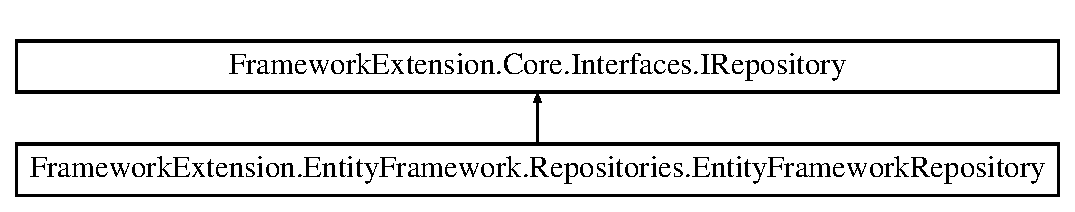
\includegraphics[height=2.000000cm]{class_framework_extension_1_1_entity_framework_1_1_repositories_1_1_entity_framework_repository}
\end{center}
\end{figure}
\subsection*{Public Member Functions}
\begin{DoxyCompactItemize}
\item 
\hypertarget{class_framework_extension_1_1_entity_framework_1_1_repositories_1_1_entity_framework_repository_a8acc429a16950d7defea2fdafa5c0a2a}{{\bfseries Entity\-Framework\-Repository} (\hyperlink{interface_framework_extension_1_1_core_1_1_interfaces_1_1_i_data_context}{I\-Data\-Context} context)}\label{class_framework_extension_1_1_entity_framework_1_1_repositories_1_1_entity_framework_repository_a8acc429a16950d7defea2fdafa5c0a2a}

\item 
T \hyperlink{class_framework_extension_1_1_entity_framework_1_1_repositories_1_1_entity_framework_repository_ad78ac84e81a696aee321145ce3c67301}{Get$<$ T $>$} (\hyperlink{interface_framework_extension_1_1_core_1_1_interfaces_1_1_i_scalar_object-g}{I\-Scalar\-Object}$<$ T $>$ query)
\begin{DoxyCompactList}\small\item\em Executes a prebuilt \hyperlink{class_i_scalar_object-g}{I\-Scalar\-Object}
\begin{DoxyTemplParams}{Template Parameters}
{\em T} & \\
\hline
\end{DoxyTemplParams}
and returns a single instance of 
\begin{DoxyTemplParams}{Template Parameters}
{\em T} & \\
\hline
\end{DoxyTemplParams}
\end{DoxyCompactList}\item 
void \hyperlink{class_framework_extension_1_1_entity_framework_1_1_repositories_1_1_entity_framework_repository_ae4fc79a4e02cf4345792dcfe917a7195}{Execute} (\hyperlink{interface_framework_extension_1_1_core_1_1_interfaces_1_1_i_command_object}{I\-Command\-Object} command)
\begin{DoxyCompactList}\small\item\em Executes a prebuilt I\-Command\-Object \end{DoxyCompactList}\item 
I\-Enumerable$<$ T $>$ \hyperlink{class_framework_extension_1_1_entity_framework_1_1_repositories_1_1_entity_framework_repository_a8c6c4a890bde5e55b6c568dfd36714b1}{Find$<$ T $>$} (\hyperlink{interface_framework_extension_1_1_core_1_1_interfaces_1_1_i_query-g}{I\-Query}$<$ T $>$ query)
\begin{DoxyCompactList}\small\item\em Executes a prebuilt \hyperlink{class_i_query-g}{I\-Query}
\begin{DoxyTemplParams}{Template Parameters}
{\em T} & \\
\hline
\end{DoxyTemplParams}
and returns an I\-Enumerable
\begin{DoxyTemplParams}{Template Parameters}
{\em T} & \\
\hline
\end{DoxyTemplParams}
\end{DoxyCompactList}\end{DoxyCompactItemize}
\subsection*{Properties}
\begin{DoxyCompactItemize}
\item 
\hyperlink{interface_framework_extension_1_1_core_1_1_interfaces_1_1_i_data_context}{I\-Data\-Context} \hyperlink{class_framework_extension_1_1_entity_framework_1_1_repositories_1_1_entity_framework_repository_ac6a6a10470ba73e14d4088fe62cf50c2}{Context}\hspace{0.3cm}{\ttfamily  \mbox{[}get, set\mbox{]}}
\begin{DoxyCompactList}\small\item\em Reference to the Context the repository is using \end{DoxyCompactList}\item 
\hyperlink{interface_framework_extension_1_1_core_1_1_interfaces_1_1_i_event_manager}{I\-Event\-Manager} \hyperlink{class_framework_extension_1_1_entity_framework_1_1_repositories_1_1_entity_framework_repository_ab8e957acbf4423a277ba2adb60eb6815}{Event\-Manager}\hspace{0.3cm}{\ttfamily  \mbox{[}get, set\mbox{]}}
\begin{DoxyCompactList}\small\item\em Reference to the Event\-Manager the repository is using \end{DoxyCompactList}\end{DoxyCompactItemize}


\subsection{Member Function Documentation}
\hypertarget{class_framework_extension_1_1_entity_framework_1_1_repositories_1_1_entity_framework_repository_ae4fc79a4e02cf4345792dcfe917a7195}{\index{Framework\-Extension\-::\-Entity\-Framework\-::\-Repositories\-::\-Entity\-Framework\-Repository@{Framework\-Extension\-::\-Entity\-Framework\-::\-Repositories\-::\-Entity\-Framework\-Repository}!Execute@{Execute}}
\index{Execute@{Execute}!FrameworkExtension::EntityFramework::Repositories::EntityFrameworkRepository@{Framework\-Extension\-::\-Entity\-Framework\-::\-Repositories\-::\-Entity\-Framework\-Repository}}
\subsubsection[{Execute}]{\setlength{\rightskip}{0pt plus 5cm}void Framework\-Extension.\-Entity\-Framework.\-Repositories.\-Entity\-Framework\-Repository.\-Execute (
\begin{DoxyParamCaption}
\item[{{\bf I\-Command\-Object}}]{command}
\end{DoxyParamCaption}
)\hspace{0.3cm}{\ttfamily [inline]}}}\label{class_framework_extension_1_1_entity_framework_1_1_repositories_1_1_entity_framework_repository_ae4fc79a4e02cf4345792dcfe917a7195}


Executes a prebuilt I\-Command\-Object 


\begin{DoxyParams}{Parameters}
{\em command} & The prebuilt command object\\
\hline
\end{DoxyParams}


Implements \hyperlink{interface_framework_extension_1_1_core_1_1_interfaces_1_1_i_repository}{Framework\-Extension.\-Core.\-Interfaces.\-I\-Repository}.

\hypertarget{class_framework_extension_1_1_entity_framework_1_1_repositories_1_1_entity_framework_repository_a8c6c4a890bde5e55b6c568dfd36714b1}{\index{Framework\-Extension\-::\-Entity\-Framework\-::\-Repositories\-::\-Entity\-Framework\-Repository@{Framework\-Extension\-::\-Entity\-Framework\-::\-Repositories\-::\-Entity\-Framework\-Repository}!Find$<$ T $>$@{Find$<$ T $>$}}
\index{Find$<$ T $>$@{Find$<$ T $>$}!FrameworkExtension::EntityFramework::Repositories::EntityFrameworkRepository@{Framework\-Extension\-::\-Entity\-Framework\-::\-Repositories\-::\-Entity\-Framework\-Repository}}
\subsubsection[{Find$<$ T $>$}]{\setlength{\rightskip}{0pt plus 5cm}I\-Enumerable$<$T$>$ Framework\-Extension.\-Entity\-Framework.\-Repositories.\-Entity\-Framework\-Repository.\-Find$<$ T $>$ (
\begin{DoxyParamCaption}
\item[{{\bf I\-Query}$<$ T $>$}]{query}
\end{DoxyParamCaption}
)\hspace{0.3cm}{\ttfamily [inline]}}}\label{class_framework_extension_1_1_entity_framework_1_1_repositories_1_1_entity_framework_repository_a8c6c4a890bde5e55b6c568dfd36714b1}


Executes a prebuilt \hyperlink{class_i_query-g}{I\-Query}
\begin{DoxyTemplParams}{Template Parameters}
{\em T} & \\
\hline
\end{DoxyTemplParams}
and returns an I\-Enumerable
\begin{DoxyTemplParams}{Template Parameters}
{\em T} & \\
\hline
\end{DoxyTemplParams}



\begin{DoxyTemplParams}{Template Parameters}
{\em T} & The Entity being queried\\
\hline
\end{DoxyTemplParams}

\begin{DoxyParams}{Parameters}
{\em query} & The prebuilt Query Object\\
\hline
\end{DoxyParams}
\begin{DoxyReturn}{Returns}
The I\-Enumerable
\begin{DoxyTemplParams}{Template Parameters}
{\em T} & \\
\hline
\end{DoxyTemplParams}
returned from the query
\end{DoxyReturn}


Implements \hyperlink{interface_framework_extension_1_1_core_1_1_interfaces_1_1_i_repository}{Framework\-Extension.\-Core.\-Interfaces.\-I\-Repository}.

\begin{Desc}
\item[Type Constraints]\begin{description}
\item[{\em T} : {\em class}]\end{description}
\end{Desc}
\hypertarget{class_framework_extension_1_1_entity_framework_1_1_repositories_1_1_entity_framework_repository_ad78ac84e81a696aee321145ce3c67301}{\index{Framework\-Extension\-::\-Entity\-Framework\-::\-Repositories\-::\-Entity\-Framework\-Repository@{Framework\-Extension\-::\-Entity\-Framework\-::\-Repositories\-::\-Entity\-Framework\-Repository}!Get$<$ T $>$@{Get$<$ T $>$}}
\index{Get$<$ T $>$@{Get$<$ T $>$}!FrameworkExtension::EntityFramework::Repositories::EntityFrameworkRepository@{Framework\-Extension\-::\-Entity\-Framework\-::\-Repositories\-::\-Entity\-Framework\-Repository}}
\subsubsection[{Get$<$ T $>$}]{\setlength{\rightskip}{0pt plus 5cm}T Framework\-Extension.\-Entity\-Framework.\-Repositories.\-Entity\-Framework\-Repository.\-Get$<$ T $>$ (
\begin{DoxyParamCaption}
\item[{{\bf I\-Scalar\-Object}$<$ T $>$}]{query}
\end{DoxyParamCaption}
)\hspace{0.3cm}{\ttfamily [inline]}}}\label{class_framework_extension_1_1_entity_framework_1_1_repositories_1_1_entity_framework_repository_ad78ac84e81a696aee321145ce3c67301}


Executes a prebuilt \hyperlink{class_i_scalar_object-g}{I\-Scalar\-Object}
\begin{DoxyTemplParams}{Template Parameters}
{\em T} & \\
\hline
\end{DoxyTemplParams}
and returns a single instance of 
\begin{DoxyTemplParams}{Template Parameters}
{\em T} & \\
\hline
\end{DoxyTemplParams}



\begin{DoxyTemplParams}{Template Parameters}
{\em T} & The Entity being queried\\
\hline
\end{DoxyTemplParams}

\begin{DoxyParams}{Parameters}
{\em query} & The prebuilt Query Object\\
\hline
\end{DoxyParams}
\begin{DoxyReturn}{Returns}
The instance of 
\begin{DoxyTemplParams}{Template Parameters}
{\em T} & \\
\hline
\end{DoxyTemplParams}
returned from the query
\end{DoxyReturn}


Implements \hyperlink{interface_framework_extension_1_1_core_1_1_interfaces_1_1_i_repository}{Framework\-Extension.\-Core.\-Interfaces.\-I\-Repository}.



\subsection{Property Documentation}
\hypertarget{class_framework_extension_1_1_entity_framework_1_1_repositories_1_1_entity_framework_repository_ac6a6a10470ba73e14d4088fe62cf50c2}{\index{Framework\-Extension\-::\-Entity\-Framework\-::\-Repositories\-::\-Entity\-Framework\-Repository@{Framework\-Extension\-::\-Entity\-Framework\-::\-Repositories\-::\-Entity\-Framework\-Repository}!Context@{Context}}
\index{Context@{Context}!FrameworkExtension::EntityFramework::Repositories::EntityFrameworkRepository@{Framework\-Extension\-::\-Entity\-Framework\-::\-Repositories\-::\-Entity\-Framework\-Repository}}
\subsubsection[{Context}]{\setlength{\rightskip}{0pt plus 5cm}{\bf I\-Data\-Context} Framework\-Extension.\-Entity\-Framework.\-Repositories.\-Entity\-Framework\-Repository.\-Context\hspace{0.3cm}{\ttfamily [get]}, {\ttfamily [set]}}}\label{class_framework_extension_1_1_entity_framework_1_1_repositories_1_1_entity_framework_repository_ac6a6a10470ba73e14d4088fe62cf50c2}


Reference to the Context the repository is using 



Implements \hyperlink{interface_framework_extension_1_1_core_1_1_interfaces_1_1_i_repository}{Framework\-Extension.\-Core.\-Interfaces.\-I\-Repository}.

\hypertarget{class_framework_extension_1_1_entity_framework_1_1_repositories_1_1_entity_framework_repository_ab8e957acbf4423a277ba2adb60eb6815}{\index{Framework\-Extension\-::\-Entity\-Framework\-::\-Repositories\-::\-Entity\-Framework\-Repository@{Framework\-Extension\-::\-Entity\-Framework\-::\-Repositories\-::\-Entity\-Framework\-Repository}!Event\-Manager@{Event\-Manager}}
\index{Event\-Manager@{Event\-Manager}!FrameworkExtension::EntityFramework::Repositories::EntityFrameworkRepository@{Framework\-Extension\-::\-Entity\-Framework\-::\-Repositories\-::\-Entity\-Framework\-Repository}}
\subsubsection[{Event\-Manager}]{\setlength{\rightskip}{0pt plus 5cm}{\bf I\-Event\-Manager} Framework\-Extension.\-Entity\-Framework.\-Repositories.\-Entity\-Framework\-Repository.\-Event\-Manager\hspace{0.3cm}{\ttfamily [get]}, {\ttfamily [set]}}}\label{class_framework_extension_1_1_entity_framework_1_1_repositories_1_1_entity_framework_repository_ab8e957acbf4423a277ba2adb60eb6815}


Reference to the Event\-Manager the repository is using 



Implements \hyperlink{interface_framework_extension_1_1_core_1_1_interfaces_1_1_i_repository}{Framework\-Extension.\-Core.\-Interfaces.\-I\-Repository}.



The documentation for this class was generated from the following file\-:\begin{DoxyCompactItemize}
\item 
Framework\-Extension.\-Entity\-Framework/\-Repositories/Entity\-Framework\-Repository.\-cs\end{DoxyCompactItemize}

\hypertarget{class_framework_extension_1_1_entity_framework_1_1_tests_1_1_unit_tests_1_1_entity_framework_test_context}{\section{Framework\-Extension.\-Entity\-Framework.\-Tests.\-Unit\-Tests.\-Entity\-Framework\-Test\-Context Class Reference}
\label{class_framework_extension_1_1_entity_framework_1_1_tests_1_1_unit_tests_1_1_entity_framework_test_context}\index{Framework\-Extension.\-Entity\-Framework.\-Tests.\-Unit\-Tests.\-Entity\-Framework\-Test\-Context@{Framework\-Extension.\-Entity\-Framework.\-Tests.\-Unit\-Tests.\-Entity\-Framework\-Test\-Context}}
}
Inheritance diagram for Framework\-Extension.\-Entity\-Framework.\-Tests.\-Unit\-Tests.\-Entity\-Framework\-Test\-Context\-:\begin{figure}[H]
\begin{center}
\leavevmode
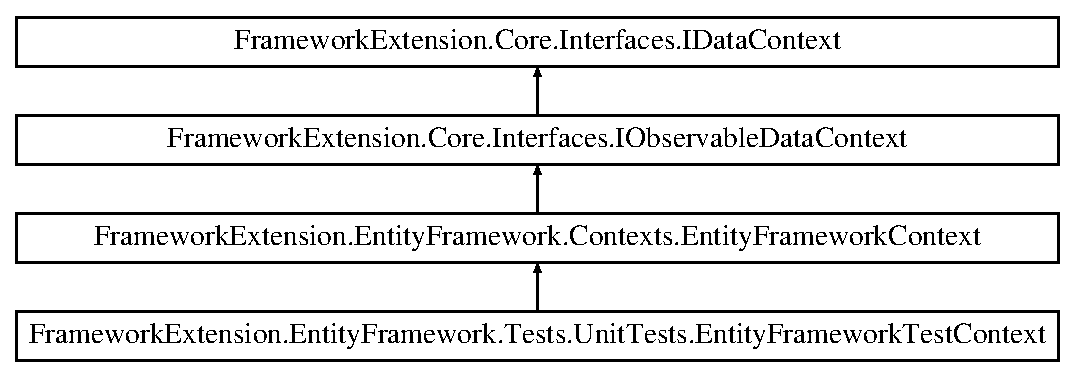
\includegraphics[height=4.000000cm]{class_framework_extension_1_1_entity_framework_1_1_tests_1_1_unit_tests_1_1_entity_framework_test_context}
\end{center}
\end{figure}
\subsection*{Public Member Functions}
\begin{DoxyCompactItemize}
\item 
\hypertarget{class_framework_extension_1_1_entity_framework_1_1_tests_1_1_unit_tests_1_1_entity_framework_test_context_a4ccb4eb34f58a8e58befcba20d05b525}{{\bfseries Entity\-Framework\-Test\-Context} (string connection\-String, \hyperlink{interface_framework_extension_1_1_entity_framework_1_1_mappings_1_1_i_mapping_configuration}{I\-Mapping\-Configuration} configuration)}\label{class_framework_extension_1_1_entity_framework_1_1_tests_1_1_unit_tests_1_1_entity_framework_test_context_a4ccb4eb34f58a8e58befcba20d05b525}

\end{DoxyCompactItemize}
\subsection*{Properties}
\begin{DoxyCompactItemize}
\item 
\hypertarget{class_framework_extension_1_1_entity_framework_1_1_tests_1_1_unit_tests_1_1_entity_framework_test_context_ab3b39185c67bbc2664808e6605180c31}{string {\bfseries Connection\-String}\hspace{0.3cm}{\ttfamily  \mbox{[}get, set\mbox{]}}}\label{class_framework_extension_1_1_entity_framework_1_1_tests_1_1_unit_tests_1_1_entity_framework_test_context_ab3b39185c67bbc2664808e6605180c31}

\end{DoxyCompactItemize}
\subsection*{Additional Inherited Members}


The documentation for this class was generated from the following file\-:\begin{DoxyCompactItemize}
\item 
Framework\-Extension.\-Entity\-Framework.\-Tests/\-Unit\-Tests/Entity\-Framework\-Test\-Context.\-cs\end{DoxyCompactItemize}

\hypertarget{class_framework_extension_1_1_core_1_1_event_management_1_1_event_manager}{\section{Framework\-Extension.\-Core.\-Event\-Management.\-Event\-Manager Class Reference}
\label{class_framework_extension_1_1_core_1_1_event_management_1_1_event_manager}\index{Framework\-Extension.\-Core.\-Event\-Management.\-Event\-Manager@{Framework\-Extension.\-Core.\-Event\-Management.\-Event\-Manager}}
}
Inheritance diagram for Framework\-Extension.\-Core.\-Event\-Management.\-Event\-Manager\-:\begin{figure}[H]
\begin{center}
\leavevmode
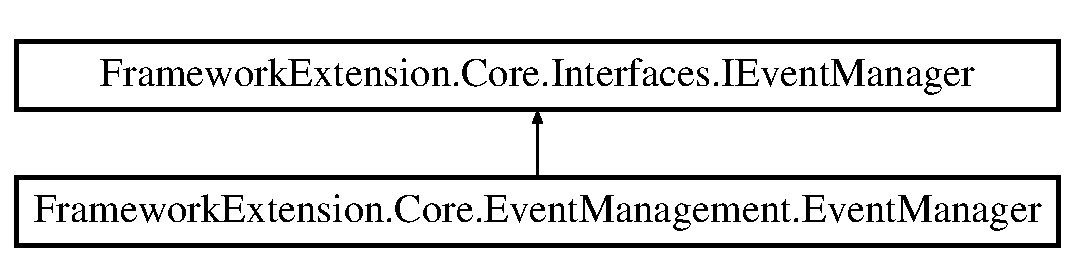
\includegraphics[height=2.000000cm]{class_framework_extension_1_1_core_1_1_event_management_1_1_event_manager}
\end{center}
\end{figure}
\subsection*{Public Member Functions}
\begin{DoxyCompactItemize}
\item 
\hypertarget{class_framework_extension_1_1_core_1_1_event_management_1_1_event_manager_a0180980ef769616dc7506c90c14fa84f}{void {\bfseries Register$<$ T $>$} (\hyperlink{interface_framework_extension_1_1_core_1_1_interfaces_1_1_i_interceptor-g}{I\-Interceptor}$<$ T $>$ interceptor)}\label{class_framework_extension_1_1_core_1_1_event_management_1_1_event_manager_a0180980ef769616dc7506c90c14fa84f}

\end{DoxyCompactItemize}
\subsection*{Properties}
\begin{DoxyCompactItemize}
\item 
\hypertarget{class_framework_extension_1_1_core_1_1_event_management_1_1_event_manager_aeb68a53416ac81a44de02512adeaec4a}{\hyperlink{interface_framework_extension_1_1_core_1_1_interfaces_1_1_i_observable_data_context}{I\-Observable\-Data\-Context} {\bfseries Context}\hspace{0.3cm}{\ttfamily  \mbox{[}get, set\mbox{]}}}\label{class_framework_extension_1_1_core_1_1_event_management_1_1_event_manager_aeb68a53416ac81a44de02512adeaec4a}

\end{DoxyCompactItemize}


The documentation for this class was generated from the following file\-:\begin{DoxyCompactItemize}
\item 
Framework\-Extension.\-Core/\-Event\-Management/Event\-Manager.\-cs\end{DoxyCompactItemize}

\hypertarget{class_m_s_test_1_1_assertion_helpers_1_1_exception_assert}{\section{M\-S\-Test.\-Assertion\-Helpers.\-Exception\-Assert Class Reference}
\label{class_m_s_test_1_1_assertion_helpers_1_1_exception_assert}\index{M\-S\-Test.\-Assertion\-Helpers.\-Exception\-Assert@{M\-S\-Test.\-Assertion\-Helpers.\-Exception\-Assert}}
}
\subsection*{Static Public Member Functions}
\begin{DoxyCompactItemize}
\item 
\hypertarget{class_m_s_test_1_1_assertion_helpers_1_1_exception_assert_acb27c67670b306400e8a68dfcc1f0101}{static void {\bfseries Throws$<$ T $>$} (Action action)}\label{class_m_s_test_1_1_assertion_helpers_1_1_exception_assert_acb27c67670b306400e8a68dfcc1f0101}

\end{DoxyCompactItemize}


The documentation for this class was generated from the following file\-:\begin{DoxyCompactItemize}
\item 
M\-S\-Test.\-Assertion\-Helpers/Exception\-Assert.\-cs\end{DoxyCompactItemize}

\hypertarget{class_framework_extension_1_1_core_1_1_test_1_1_test_domain_1_1_foo}{\section{Framework\-Extension.\-Core.\-Test.\-Test\-Domain.\-Foo Class Reference}
\label{class_framework_extension_1_1_core_1_1_test_1_1_test_domain_1_1_foo}\index{Framework\-Extension.\-Core.\-Test.\-Test\-Domain.\-Foo@{Framework\-Extension.\-Core.\-Test.\-Test\-Domain.\-Foo}}
}
\subsection*{Properties}
\begin{DoxyCompactItemize}
\item 
\hypertarget{class_framework_extension_1_1_core_1_1_test_1_1_test_domain_1_1_foo_adbda4bf8d3a7ed8e9c4f5db100f367b0}{int {\bfseries Id}\hspace{0.3cm}{\ttfamily  \mbox{[}get, set\mbox{]}}}\label{class_framework_extension_1_1_core_1_1_test_1_1_test_domain_1_1_foo_adbda4bf8d3a7ed8e9c4f5db100f367b0}

\item 
\hypertarget{class_framework_extension_1_1_core_1_1_test_1_1_test_domain_1_1_foo_a1b045c518e71d4ee187ab16c31230a81}{string {\bfseries Name}\hspace{0.3cm}{\ttfamily  \mbox{[}get, set\mbox{]}}}\label{class_framework_extension_1_1_core_1_1_test_1_1_test_domain_1_1_foo_a1b045c518e71d4ee187ab16c31230a81}

\end{DoxyCompactItemize}


The documentation for this class was generated from the following file\-:\begin{DoxyCompactItemize}
\item 
Framework\-Extension.\-Core.\-Test/\-Test\-Domain/Foo.\-cs\end{DoxyCompactItemize}

\hypertarget{class_framework_extension_1_1_entity_framework_1_1_tests_1_1_mapping_1_1_foo_map}{\section{Framework\-Extension.\-Entity\-Framework.\-Tests.\-Mapping.\-Foo\-Map Class Reference}
\label{class_framework_extension_1_1_entity_framework_1_1_tests_1_1_mapping_1_1_foo_map}\index{Framework\-Extension.\-Entity\-Framework.\-Tests.\-Mapping.\-Foo\-Map@{Framework\-Extension.\-Entity\-Framework.\-Tests.\-Mapping.\-Foo\-Map}}
}


The documentation for this class was generated from the following file\-:\begin{DoxyCompactItemize}
\item 
Framework\-Extension.\-Entity\-Framework.\-Tests/\-Mapping/Foo\-Map.\-cs\end{DoxyCompactItemize}

\hypertarget{class_framework_extension_1_1_entity_framework_1_1_tests_1_1_initializer_1_1_force_delete_initializer}{\section{Framework\-Extension.\-Entity\-Framework.\-Tests.\-Initializer.\-Force\-Delete\-Initializer Class Reference}
\label{class_framework_extension_1_1_entity_framework_1_1_tests_1_1_initializer_1_1_force_delete_initializer}\index{Framework\-Extension.\-Entity\-Framework.\-Tests.\-Initializer.\-Force\-Delete\-Initializer@{Framework\-Extension.\-Entity\-Framework.\-Tests.\-Initializer.\-Force\-Delete\-Initializer}}
}
\subsection*{Public Member Functions}
\begin{DoxyCompactItemize}
\item 
\hypertarget{class_framework_extension_1_1_entity_framework_1_1_tests_1_1_initializer_1_1_force_delete_initializer_aaa356804097e887596e42aceee560ec1}{{\bfseries Force\-Delete\-Initializer} (I\-Database\-Initializer$<$ \hyperlink{class_framework_extension_1_1_entity_framework_1_1_tests_1_1_unit_tests_1_1_entity_framework_test_context}{Entity\-Framework\-Test\-Context} $>$ inner\-Initializer)}\label{class_framework_extension_1_1_entity_framework_1_1_tests_1_1_initializer_1_1_force_delete_initializer_aaa356804097e887596e42aceee560ec1}

\item 
\hypertarget{class_framework_extension_1_1_entity_framework_1_1_tests_1_1_initializer_1_1_force_delete_initializer_a276504ce4d33743ff35377c971af3dce}{void {\bfseries Initialize\-Database} (\hyperlink{class_framework_extension_1_1_entity_framework_1_1_tests_1_1_unit_tests_1_1_entity_framework_test_context}{Entity\-Framework\-Test\-Context} context)}\label{class_framework_extension_1_1_entity_framework_1_1_tests_1_1_initializer_1_1_force_delete_initializer_a276504ce4d33743ff35377c971af3dce}

\end{DoxyCompactItemize}


The documentation for this class was generated from the following file\-:\begin{DoxyCompactItemize}
\item 
Framework\-Extension.\-Entity\-Framework.\-Tests/\-Initializer/Entity\-Framework\-Intializer.\-cs\end{DoxyCompactItemize}

\hypertarget{class_framework_extension_1_1_entity_framework_1_1_tests_1_1_unit_tests_1_1_given___a___collection___of___t}{\section{Framework\-Extension.\-Entity\-Framework.\-Tests.\-Unit\-Tests.\-Given\-\_\-\-A\-\_\-\-Collection\-\_\-\-Of\-\_\-\-T Class Reference}
\label{class_framework_extension_1_1_entity_framework_1_1_tests_1_1_unit_tests_1_1_given___a___collection___of___t}\index{Framework\-Extension.\-Entity\-Framework.\-Tests.\-Unit\-Tests.\-Given\-\_\-\-A\-\_\-\-Collection\-\_\-\-Of\-\_\-\-T@{Framework\-Extension.\-Entity\-Framework.\-Tests.\-Unit\-Tests.\-Given\-\_\-\-A\-\_\-\-Collection\-\_\-\-Of\-\_\-\-T}}
}
\subsection*{Classes}
\begin{DoxyCompactItemize}
\item 
class {\bfseries Test\-Action\-Holder}
\end{DoxyCompactItemize}
\subsection*{Public Member Functions}
\begin{DoxyCompactItemize}
\item 
\hypertarget{class_framework_extension_1_1_entity_framework_1_1_tests_1_1_unit_tests_1_1_given___a___collection___of___t_a26dfbbbbf943d834726f63567c45d7ca}{void {\bfseries When\-\_\-\-Each\-\_\-\-Is\-\_\-\-Called\-\_\-\-Action\-\_\-\-Gets\-\_\-invoked\-\_\-for\-\_\-every\-\_\-item} ()}\label{class_framework_extension_1_1_entity_framework_1_1_tests_1_1_unit_tests_1_1_given___a___collection___of___t_a26dfbbbbf943d834726f63567c45d7ca}

\end{DoxyCompactItemize}


The documentation for this class was generated from the following file\-:\begin{DoxyCompactItemize}
\item 
Framework\-Extension.\-Entity\-Framework.\-Tests/\-Unit\-Tests/Given\-\_\-\-A\-\_\-\-Collection\-\_\-\-Of\-\_\-\-T.\-cs\end{DoxyCompactItemize}

\hypertarget{class_framework_extension_1_1_entity_framework_1_1_tests_1_1_unit_tests_1_1_given___a___context___without___mappings}{\section{Framework\-Extension.\-Entity\-Framework.\-Tests.\-Unit\-Tests.\-Given\-\_\-\-A\-\_\-\-Context\-\_\-\-Without\-\_\-\-Mappings Class Reference}
\label{class_framework_extension_1_1_entity_framework_1_1_tests_1_1_unit_tests_1_1_given___a___context___without___mappings}\index{Framework\-Extension.\-Entity\-Framework.\-Tests.\-Unit\-Tests.\-Given\-\_\-\-A\-\_\-\-Context\-\_\-\-Without\-\_\-\-Mappings@{Framework\-Extension.\-Entity\-Framework.\-Tests.\-Unit\-Tests.\-Given\-\_\-\-A\-\_\-\-Context\-\_\-\-Without\-\_\-\-Mappings}}
}
\subsection*{Public Member Functions}
\begin{DoxyCompactItemize}
\item 
\hypertarget{class_framework_extension_1_1_entity_framework_1_1_tests_1_1_unit_tests_1_1_given___a___context___without___mappings_adf294b9193cd744039bbf9b5a3e5c6fa}{void {\bfseries Mappings\-\_\-\-Can\-\_\-\-Be\-\_\-\-Injected\-\_\-instead\-\_\-of\-\_\-explicitly\-\_\-coded\-\_\-in\-\_\-the\-\_\-context} ()}\label{class_framework_extension_1_1_entity_framework_1_1_tests_1_1_unit_tests_1_1_given___a___context___without___mappings_adf294b9193cd744039bbf9b5a3e5c6fa}

\end{DoxyCompactItemize}


The documentation for this class was generated from the following file\-:\begin{DoxyCompactItemize}
\item 
Framework\-Extension.\-Entity\-Framework.\-Tests/\-Unit\-Tests/Given\-\_\-\-A\-\_\-\-Context\-\_\-\-Without\-\_\-\-Mappings.\-cs\end{DoxyCompactItemize}

\hypertarget{class_framework_extension_1_1_entity_framework_1_1_tests_1_1_integration_tests_1_1_given___a___e_f___context}{\section{Framework\-Extension.\-Entity\-Framework.\-Tests.\-Integration\-Tests.\-Given\-\_\-\-A\-\_\-\-E\-F\-\_\-\-Context Class Reference}
\label{class_framework_extension_1_1_entity_framework_1_1_tests_1_1_integration_tests_1_1_given___a___e_f___context}\index{Framework\-Extension.\-Entity\-Framework.\-Tests.\-Integration\-Tests.\-Given\-\_\-\-A\-\_\-\-E\-F\-\_\-\-Context@{Framework\-Extension.\-Entity\-Framework.\-Tests.\-Integration\-Tests.\-Given\-\_\-\-A\-\_\-\-E\-F\-\_\-\-Context}}
}
\subsection*{Public Member Functions}
\begin{DoxyCompactItemize}
\item 
\hypertarget{class_framework_extension_1_1_entity_framework_1_1_tests_1_1_integration_tests_1_1_given___a___e_f___context_a50d5c6c99069c4ab842faa674d1c8ab3}{void {\bfseries Setup} ()}\label{class_framework_extension_1_1_entity_framework_1_1_tests_1_1_integration_tests_1_1_given___a___e_f___context_a50d5c6c99069c4ab842faa674d1c8ab3}

\item 
\hypertarget{class_framework_extension_1_1_entity_framework_1_1_tests_1_1_integration_tests_1_1_given___a___e_f___context_ad22683b340548579f36e2000defa3598}{void {\bfseries When\-\_\-\-As\-Queryable\-\_\-\-Called\-\_\-\-A\-\_\-\-Set\-\_\-\-Is\-\_\-\-Pulled\-\_\-\-From\-\_\-\-The\-\_\-\-Database} ()}\label{class_framework_extension_1_1_entity_framework_1_1_tests_1_1_integration_tests_1_1_given___a___e_f___context_ad22683b340548579f36e2000defa3598}

\item 
\hypertarget{class_framework_extension_1_1_entity_framework_1_1_tests_1_1_integration_tests_1_1_given___a___e_f___context_ab7514aa42cb41b3d9d9de15be0541134}{void {\bfseries When\-\_\-\-Add\-\_\-\-Is\-\_\-\-Called\-\_\-\-The\-\_\-\-Object\-\_\-\-Is\-\_\-\-Added\-\_\-\-To\-\_\-\-The\-\_\-\-Change\-Tracker\-\_\-\-In\-\_\-\-An\-\_\-\-Added\-\_\-\-State} ()}\label{class_framework_extension_1_1_entity_framework_1_1_tests_1_1_integration_tests_1_1_given___a___e_f___context_ab7514aa42cb41b3d9d9de15be0541134}

\item 
\hypertarget{class_framework_extension_1_1_entity_framework_1_1_tests_1_1_integration_tests_1_1_given___a___e_f___context_a296f426aaaca7ec67f09292bba69bab7}{void {\bfseries When\-\_\-\-Remove\-\_\-\-Is\-\_\-\-Called\-\_\-\-The\-\_\-\-Object\-\_\-\-Is\-\_\-\-Added\-\_\-\-To\-\_\-\-The\-\_\-\-Change\-Tracker\-\_\-\-In\-\_\-\-A\-\_\-\-Deleted\-\_\-\-State} ()}\label{class_framework_extension_1_1_entity_framework_1_1_tests_1_1_integration_tests_1_1_given___a___e_f___context_a296f426aaaca7ec67f09292bba69bab7}

\item 
\hypertarget{class_framework_extension_1_1_entity_framework_1_1_tests_1_1_integration_tests_1_1_given___a___e_f___context_a2fe0d758e38ff2b76fdadf317318d1a0}{void {\bfseries When\-\_\-\-Detach\-\_\-\-Is\-\_\-\-Called\-\_\-\-The\-\_\-\-Object\-\_\-\-Is\-\_\-\-Added\-\_\-\-To\-\_\-\-The\-\_\-\-Change\-Tracker\-\_\-\-In\-\_\-\-A\-\_\-\-Detached\-\_\-\-State} ()}\label{class_framework_extension_1_1_entity_framework_1_1_tests_1_1_integration_tests_1_1_given___a___e_f___context_a2fe0d758e38ff2b76fdadf317318d1a0}

\end{DoxyCompactItemize}
\subsection*{Static Public Member Functions}
\begin{DoxyCompactItemize}
\item 
\hypertarget{class_framework_extension_1_1_entity_framework_1_1_tests_1_1_integration_tests_1_1_given___a___e_f___context_a633632ed97bf8f7aa2577a419df6bed2}{static void {\bfseries Setup\-Class} (Test\-Context context)}\label{class_framework_extension_1_1_entity_framework_1_1_tests_1_1_integration_tests_1_1_given___a___e_f___context_a633632ed97bf8f7aa2577a419df6bed2}

\end{DoxyCompactItemize}


The documentation for this class was generated from the following file\-:\begin{DoxyCompactItemize}
\item 
Framework\-Extension.\-Entity\-Framework.\-Tests/\-Integration\-Tests/Given\-\_\-\-A\-\_\-\-E\-F\-\_\-\-Context.\-cs\end{DoxyCompactItemize}

\hypertarget{class_framework_extension_1_1_entity_framework_1_1_tests_1_1_unit_tests_1_1_given___a___generic___repository}{\section{Framework\-Extension.\-Entity\-Framework.\-Tests.\-Unit\-Tests.\-Given\-\_\-\-A\-\_\-\-Generic\-\_\-\-Repository Class Reference}
\label{class_framework_extension_1_1_entity_framework_1_1_tests_1_1_unit_tests_1_1_given___a___generic___repository}\index{Framework\-Extension.\-Entity\-Framework.\-Tests.\-Unit\-Tests.\-Given\-\_\-\-A\-\_\-\-Generic\-\_\-\-Repository@{Framework\-Extension.\-Entity\-Framework.\-Tests.\-Unit\-Tests.\-Given\-\_\-\-A\-\_\-\-Generic\-\_\-\-Repository}}
}
\subsection*{Public Member Functions}
\begin{DoxyCompactItemize}
\item 
\hypertarget{class_framework_extension_1_1_entity_framework_1_1_tests_1_1_unit_tests_1_1_given___a___generic___repository_ac152ff77e79bc18befb40f2f38bca218}{void {\bfseries When\-\_\-\-Given\-\_\-\-A\-\_\-\-Contructor\-\_\-\-It\-\_\-\-Should\-\_\-\-Support\-\_\-\-Dependency\-\_\-\-Injection} ()}\label{class_framework_extension_1_1_entity_framework_1_1_tests_1_1_unit_tests_1_1_given___a___generic___repository_ac152ff77e79bc18befb40f2f38bca218}

\item 
\hypertarget{class_framework_extension_1_1_entity_framework_1_1_tests_1_1_unit_tests_1_1_given___a___generic___repository_aa239cd9107eba961105c741064b00d3d}{void {\bfseries Should\-\_\-\-Execute\-\_\-\-Query\-\_\-\-Objects} ()}\label{class_framework_extension_1_1_entity_framework_1_1_tests_1_1_unit_tests_1_1_given___a___generic___repository_aa239cd9107eba961105c741064b00d3d}

\item 
\hypertarget{class_framework_extension_1_1_entity_framework_1_1_tests_1_1_unit_tests_1_1_given___a___generic___repository_ab08819451bb3dc341cd7da033e7d7b9d}{void {\bfseries Should\-\_\-\-Execute\-\_\-\-Scalar\-\_\-\-Objects\-\_\-\-That\-\_\-\-Return\-\_\-\-Values} ()}\label{class_framework_extension_1_1_entity_framework_1_1_tests_1_1_unit_tests_1_1_given___a___generic___repository_ab08819451bb3dc341cd7da033e7d7b9d}

\item 
\hypertarget{class_framework_extension_1_1_entity_framework_1_1_tests_1_1_unit_tests_1_1_given___a___generic___repository_aefd92e774733e5b6aacd062b72588675}{void {\bfseries Should\-\_\-\-Execute\-\_\-\-Scalar\-\_\-\-Objects\-\_\-\-That\-\_\-\-Return\-\_\-\-Objects} ()}\label{class_framework_extension_1_1_entity_framework_1_1_tests_1_1_unit_tests_1_1_given___a___generic___repository_aefd92e774733e5b6aacd062b72588675}

\item 
\hypertarget{class_framework_extension_1_1_entity_framework_1_1_tests_1_1_unit_tests_1_1_given___a___generic___repository_a74d111be27574908b2c70fc660ec7335}{void {\bfseries Should\-\_\-\-Execute\-\_\-\-A\-\_\-\-Query\-\_\-\-Object\-\_\-\-And\-\_\-\-Pull\-\_\-\-The\-\_\-\-First\-\_\-\-Object} ()}\label{class_framework_extension_1_1_entity_framework_1_1_tests_1_1_unit_tests_1_1_given___a___generic___repository_a74d111be27574908b2c70fc660ec7335}

\item 
\hypertarget{class_framework_extension_1_1_entity_framework_1_1_tests_1_1_unit_tests_1_1_given___a___generic___repository_a28a89885537c7eda8d34a63da535b213}{void {\bfseries Should\-\_\-\-Execute\-\_\-\-Commands\-\_\-\-Against\-\_\-\-Context} ()}\label{class_framework_extension_1_1_entity_framework_1_1_tests_1_1_unit_tests_1_1_given___a___generic___repository_a28a89885537c7eda8d34a63da535b213}

\end{DoxyCompactItemize}
\subsection*{Static Public Member Functions}
\begin{DoxyCompactItemize}
\item 
\hypertarget{class_framework_extension_1_1_entity_framework_1_1_tests_1_1_unit_tests_1_1_given___a___generic___repository_ac6db1e47fe3a0226be21393b8b5a69fe}{static void {\bfseries Setup\-Class} (Test\-Context context)}\label{class_framework_extension_1_1_entity_framework_1_1_tests_1_1_unit_tests_1_1_given___a___generic___repository_ac6db1e47fe3a0226be21393b8b5a69fe}

\end{DoxyCompactItemize}


The documentation for this class was generated from the following file\-:\begin{DoxyCompactItemize}
\item 
Framework\-Extension.\-Entity\-Framework.\-Tests/\-Unit\-Tests/Given\-\_\-\-A\-\_\-\-Generic\-\_\-\-Repository.\-cs\end{DoxyCompactItemize}

\hypertarget{class_framework_extension_1_1_entity_framework_1_1_tests_1_1_unit_tests_1_1_given___a___query___object}{\section{Framework\-Extension.\-Entity\-Framework.\-Tests.\-Unit\-Tests.\-Given\-\_\-\-A\-\_\-\-Query\-\_\-\-Object Class Reference}
\label{class_framework_extension_1_1_entity_framework_1_1_tests_1_1_unit_tests_1_1_given___a___query___object}\index{Framework\-Extension.\-Entity\-Framework.\-Tests.\-Unit\-Tests.\-Given\-\_\-\-A\-\_\-\-Query\-\_\-\-Object@{Framework\-Extension.\-Entity\-Framework.\-Tests.\-Unit\-Tests.\-Given\-\_\-\-A\-\_\-\-Query\-\_\-\-Object}}
}
\subsection*{Public Member Functions}
\begin{DoxyCompactItemize}
\item 
\hypertarget{class_framework_extension_1_1_entity_framework_1_1_tests_1_1_unit_tests_1_1_given___a___query___object_a32af6d21858a66e33efea6bebb8f9aa1}{void {\bfseries When\-\_\-\-Passing\-\_\-\-To\-\_\-\-A\-\_\-\-Repository\-\_\-\-Query\-\_\-\-Object\-\_\-\-Then\-\_\-\-It\-\_\-\-Executes\-\_\-\-Against\-\_\-\-Context} ()}\label{class_framework_extension_1_1_entity_framework_1_1_tests_1_1_unit_tests_1_1_given___a___query___object_a32af6d21858a66e33efea6bebb8f9aa1}

\item 
\hypertarget{class_framework_extension_1_1_entity_framework_1_1_tests_1_1_unit_tests_1_1_given___a___query___object_a70e5ae60941103978d0bd592f2dff2a2}{void {\bfseries When\-\_\-\-Executed\-\_\-\-Returns\-\_\-\-An\-\_\-\-I\-Enumerable\-\_\-\-Of\-\_\-\-Items} ()}\label{class_framework_extension_1_1_entity_framework_1_1_tests_1_1_unit_tests_1_1_given___a___query___object_a70e5ae60941103978d0bd592f2dff2a2}

\item 
\hypertarget{class_framework_extension_1_1_entity_framework_1_1_tests_1_1_unit_tests_1_1_given___a___query___object_a84042acb712a792a38f9369cc8d2a6bc}{void {\bfseries When\-\_\-\-Paging\-\_\-\-Should\-\_\-\-Affect\-\_\-\-The\-\_\-\-Base\-\_\-\-Query\-\_\-\-Before\-\_\-\-It\-\_\-\-Is\-\_\-\-Executed} ()}\label{class_framework_extension_1_1_entity_framework_1_1_tests_1_1_unit_tests_1_1_given___a___query___object_a84042acb712a792a38f9369cc8d2a6bc}

\item 
\hypertarget{class_framework_extension_1_1_entity_framework_1_1_tests_1_1_unit_tests_1_1_given___a___query___object_a4b1dc3d91a71db13bc265ace09aee372}{void {\bfseries When\-\_\-\-Calling\-\_\-\-Output\-\_\-\-Sql\-\_\-with\-\_\-\-Context\-\_\-\-It\-\_\-\-Outputs\-\_\-\-S\-Q\-L} ()}\label{class_framework_extension_1_1_entity_framework_1_1_tests_1_1_unit_tests_1_1_given___a___query___object_a4b1dc3d91a71db13bc265ace09aee372}

\end{DoxyCompactItemize}
\subsection*{Static Public Member Functions}
\begin{DoxyCompactItemize}
\item 
\hypertarget{class_framework_extension_1_1_entity_framework_1_1_tests_1_1_unit_tests_1_1_given___a___query___object_ac56086e9c84a2d46794d66dc33c7d10c}{static void {\bfseries Setup\-Class} (Test\-Context context)}\label{class_framework_extension_1_1_entity_framework_1_1_tests_1_1_unit_tests_1_1_given___a___query___object_ac56086e9c84a2d46794d66dc33c7d10c}

\end{DoxyCompactItemize}


The documentation for this class was generated from the following file\-:\begin{DoxyCompactItemize}
\item 
Framework\-Extension.\-Entity\-Framework.\-Tests/\-Unit\-Tests/Given\-\_\-\-A\-\_\-\-Query\-\_\-\-Object.\-cs\end{DoxyCompactItemize}

\hypertarget{class_framework_extension_1_1_entity_framework_1_1_tests_1_1_unit_tests_1_1_given___a___scalar___object}{\section{Framework\-Extension.\-Entity\-Framework.\-Tests.\-Unit\-Tests.\-Given\-\_\-\-A\-\_\-\-Scalar\-\_\-\-Object Class Reference}
\label{class_framework_extension_1_1_entity_framework_1_1_tests_1_1_unit_tests_1_1_given___a___scalar___object}\index{Framework\-Extension.\-Entity\-Framework.\-Tests.\-Unit\-Tests.\-Given\-\_\-\-A\-\_\-\-Scalar\-\_\-\-Object@{Framework\-Extension.\-Entity\-Framework.\-Tests.\-Unit\-Tests.\-Given\-\_\-\-A\-\_\-\-Scalar\-\_\-\-Object}}
}
\subsection*{Public Member Functions}
\begin{DoxyCompactItemize}
\item 
\hypertarget{class_framework_extension_1_1_entity_framework_1_1_tests_1_1_unit_tests_1_1_given___a___scalar___object_a863da0b1f8d23ac9d88f98a005bb0665}{void {\bfseries When\-\_\-\-Passing\-\_\-\-To\-\_\-\-A\-\_\-\-Repository\-\_\-\-Scalar\-\_\-\-Object\-\_\-\-Then\-\_\-\-It\-\_\-\-Executes\-\_\-\-Against\-\_\-\-Context} ()}\label{class_framework_extension_1_1_entity_framework_1_1_tests_1_1_unit_tests_1_1_given___a___scalar___object_a863da0b1f8d23ac9d88f98a005bb0665}

\item 
\hypertarget{class_framework_extension_1_1_entity_framework_1_1_tests_1_1_unit_tests_1_1_given___a___scalar___object_a4e561f4e4ea40f556495bd8773e979fb}{void {\bfseries When\-\_\-\-Executed\-\_\-\-Returns\-\_\-\-A\-\_\-\-Single\-\_\-\-Value} ()}\label{class_framework_extension_1_1_entity_framework_1_1_tests_1_1_unit_tests_1_1_given___a___scalar___object_a4e561f4e4ea40f556495bd8773e979fb}

\end{DoxyCompactItemize}
\subsection*{Static Public Member Functions}
\begin{DoxyCompactItemize}
\item 
\hypertarget{class_framework_extension_1_1_entity_framework_1_1_tests_1_1_unit_tests_1_1_given___a___scalar___object_ab3aeaff417f2f8e98b74754fc7c2ec3b}{static void {\bfseries Setup\-Class} (Test\-Context context)}\label{class_framework_extension_1_1_entity_framework_1_1_tests_1_1_unit_tests_1_1_given___a___scalar___object_ab3aeaff417f2f8e98b74754fc7c2ec3b}

\end{DoxyCompactItemize}


The documentation for this class was generated from the following file\-:\begin{DoxyCompactItemize}
\item 
Framework\-Extension.\-Entity\-Framework.\-Tests/\-Unit\-Tests/Given\-\_\-\-A\-\_\-\-Scalar\-\_\-\-Object.\-cs\end{DoxyCompactItemize}

\hypertarget{class_framework_extension_1_1_entity_framework_1_1_tests_1_1_unit_tests_1_1_given___an___event___extendable___context}{\section{Framework\-Extension.\-Entity\-Framework.\-Tests.\-Unit\-Tests.\-Given\-\_\-\-An\-\_\-\-Event\-\_\-\-Extendable\-\_\-\-Context Class Reference}
\label{class_framework_extension_1_1_entity_framework_1_1_tests_1_1_unit_tests_1_1_given___an___event___extendable___context}\index{Framework\-Extension.\-Entity\-Framework.\-Tests.\-Unit\-Tests.\-Given\-\_\-\-An\-\_\-\-Event\-\_\-\-Extendable\-\_\-\-Context@{Framework\-Extension.\-Entity\-Framework.\-Tests.\-Unit\-Tests.\-Given\-\_\-\-An\-\_\-\-Event\-\_\-\-Extendable\-\_\-\-Context}}
}
\subsection*{Public Member Functions}
\begin{DoxyCompactItemize}
\item 
\hypertarget{class_framework_extension_1_1_entity_framework_1_1_tests_1_1_unit_tests_1_1_given___an___event___extendable___context_a0060725c30d3161b46bc5463e83d213b}{void {\bfseries When\-\_\-\-Commit\-\_\-\-Is\-\_\-\-Called\-\_\-\-Pre\-Save\-\_\-and\-\_\-post\-\_\-save\-\_\-interceptors\-\_\-are\-\_\-\-Called} ()}\label{class_framework_extension_1_1_entity_framework_1_1_tests_1_1_unit_tests_1_1_given___an___event___extendable___context_a0060725c30d3161b46bc5463e83d213b}

\end{DoxyCompactItemize}


The documentation for this class was generated from the following file\-:\begin{DoxyCompactItemize}
\item 
Framework\-Extension.\-Entity\-Framework.\-Tests/\-Unit\-Tests/Given\-\_\-\-An\-\_\-\-Event\-\_\-\-Extendable\-\_\-\-Context.\-cs\end{DoxyCompactItemize}

\hypertarget{interface_framework_extension_1_1_core_1_1_interfaces_1_1_i_auditable_entity}{\section{Framework\-Extension.\-Core.\-Interfaces.\-I\-Auditable\-Entity Interface Reference}
\label{interface_framework_extension_1_1_core_1_1_interfaces_1_1_i_auditable_entity}\index{Framework\-Extension.\-Core.\-Interfaces.\-I\-Auditable\-Entity@{Framework\-Extension.\-Core.\-Interfaces.\-I\-Auditable\-Entity}}
}
\subsection*{Properties}
\begin{DoxyCompactItemize}
\item 
\hypertarget{interface_framework_extension_1_1_core_1_1_interfaces_1_1_i_auditable_entity_aad7433e3f83ee4717646b934ac99e39f}{Date\-Time {\bfseries Created\-Date}\hspace{0.3cm}{\ttfamily  \mbox{[}get, set\mbox{]}}}\label{interface_framework_extension_1_1_core_1_1_interfaces_1_1_i_auditable_entity_aad7433e3f83ee4717646b934ac99e39f}

\item 
\hypertarget{interface_framework_extension_1_1_core_1_1_interfaces_1_1_i_auditable_entity_a6377d54897523ff616b9575b04fad762}{string {\bfseries Created\-By}\hspace{0.3cm}{\ttfamily  \mbox{[}get, set\mbox{]}}}\label{interface_framework_extension_1_1_core_1_1_interfaces_1_1_i_auditable_entity_a6377d54897523ff616b9575b04fad762}

\item 
\hypertarget{interface_framework_extension_1_1_core_1_1_interfaces_1_1_i_auditable_entity_ab615ce49f19a49dd7d6643df0a25baa0}{Date\-Time {\bfseries Modified\-Date}\hspace{0.3cm}{\ttfamily  \mbox{[}get, set\mbox{]}}}\label{interface_framework_extension_1_1_core_1_1_interfaces_1_1_i_auditable_entity_ab615ce49f19a49dd7d6643df0a25baa0}

\item 
\hypertarget{interface_framework_extension_1_1_core_1_1_interfaces_1_1_i_auditable_entity_a70ba9dabc0c90989a09b8d319ec18888}{string {\bfseries Modified\-By}\hspace{0.3cm}{\ttfamily  \mbox{[}get, set\mbox{]}}}\label{interface_framework_extension_1_1_core_1_1_interfaces_1_1_i_auditable_entity_a70ba9dabc0c90989a09b8d319ec18888}

\end{DoxyCompactItemize}


The documentation for this interface was generated from the following file\-:\begin{DoxyCompactItemize}
\item 
Framework\-Extension.\-Core/\-Interfaces/I\-Auditable\-Entity.\-cs\end{DoxyCompactItemize}

\hypertarget{interface_framework_extension_1_1_core_1_1_interfaces_1_1_i_command_object}{\section{Framework\-Extension.\-Core.\-Interfaces.\-I\-Command\-Object Interface Reference}
\label{interface_framework_extension_1_1_core_1_1_interfaces_1_1_i_command_object}\index{Framework\-Extension.\-Core.\-Interfaces.\-I\-Command\-Object@{Framework\-Extension.\-Core.\-Interfaces.\-I\-Command\-Object}}
}
Inheritance diagram for Framework\-Extension.\-Core.\-Interfaces.\-I\-Command\-Object\-:\begin{figure}[H]
\begin{center}
\leavevmode
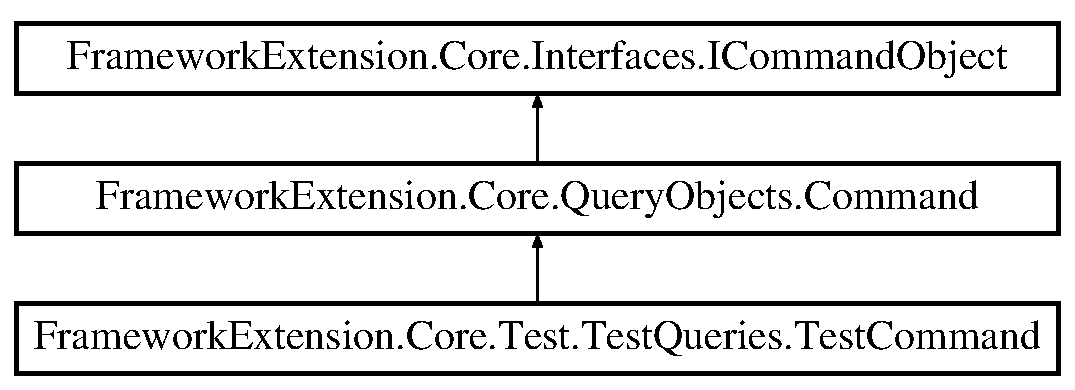
\includegraphics[height=3.000000cm]{interface_framework_extension_1_1_core_1_1_interfaces_1_1_i_command_object}
\end{center}
\end{figure}
\subsection*{Public Member Functions}
\begin{DoxyCompactItemize}
\item 
\hypertarget{interface_framework_extension_1_1_core_1_1_interfaces_1_1_i_command_object_a4e41bd2594aa5c7902bb03cd0bd002bc}{void {\bfseries Execute} (\hyperlink{interface_framework_extension_1_1_core_1_1_interfaces_1_1_i_data_context}{I\-Data\-Context} context)}\label{interface_framework_extension_1_1_core_1_1_interfaces_1_1_i_command_object_a4e41bd2594aa5c7902bb03cd0bd002bc}

\end{DoxyCompactItemize}


The documentation for this interface was generated from the following file\-:\begin{DoxyCompactItemize}
\item 
Framework\-Extension.\-Core/\-Interfaces/I\-Query.\-cs\end{DoxyCompactItemize}

\hypertarget{interface_framework_extension_1_1_core_1_1_interfaces_1_1_i_data_context}{\section{Framework\-Extension.\-Core.\-Interfaces.\-I\-Data\-Context Interface Reference}
\label{interface_framework_extension_1_1_core_1_1_interfaces_1_1_i_data_context}\index{Framework\-Extension.\-Core.\-Interfaces.\-I\-Data\-Context@{Framework\-Extension.\-Core.\-Interfaces.\-I\-Data\-Context}}
}
Inheritance diagram for Framework\-Extension.\-Core.\-Interfaces.\-I\-Data\-Context\-:\begin{figure}[H]
\begin{center}
\leavevmode
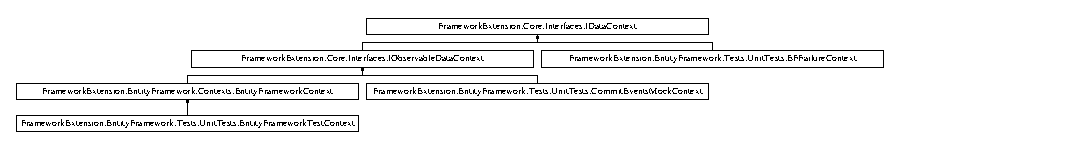
\includegraphics[height=1.539519cm]{interface_framework_extension_1_1_core_1_1_interfaces_1_1_i_data_context}
\end{center}
\end{figure}
\subsection*{Public Member Functions}
\begin{DoxyCompactItemize}
\item 
I\-Queryable$<$ T $>$ \hyperlink{interface_framework_extension_1_1_core_1_1_interfaces_1_1_i_data_context_a815dee1d6eb11910fc12250752b654b7}{As\-Queryable$<$ T $>$} ()
\begin{DoxyCompactList}\small\item\em This gives a mockable wrapper around the normal Set
\begin{DoxyTemplParams}{Template Parameters}
{\em T} & \\
\hline
\end{DoxyTemplParams}
method that allows for testablity \end{DoxyCompactList}\item 
T \hyperlink{interface_framework_extension_1_1_core_1_1_interfaces_1_1_i_data_context_a0c8685ab4b1c99f897eba29fba179896}{Add$<$ T $>$} (T item)
\begin{DoxyCompactList}\small\item\em Adds the provided instance of 
\begin{DoxyTemplParams}{Template Parameters}
{\em T} & \\
\hline
\end{DoxyTemplParams}
to the data context \end{DoxyCompactList}\item 
T \hyperlink{interface_framework_extension_1_1_core_1_1_interfaces_1_1_i_data_context_a713205a05d584b6d47325434e6723564}{Remove$<$ T $>$} (T item)
\begin{DoxyCompactList}\small\item\em Removes the provided instance of 
\begin{DoxyTemplParams}{Template Parameters}
{\em T} & \\
\hline
\end{DoxyTemplParams}
from the data context \end{DoxyCompactList}\item 
T \hyperlink{interface_framework_extension_1_1_core_1_1_interfaces_1_1_i_data_context_a1297c0d6e59ec05855d8e25a72f49fdd}{Update$<$ T $>$} (T item)
\begin{DoxyCompactList}\small\item\em Updates the provided instance of 
\begin{DoxyTemplParams}{Template Parameters}
{\em T} & \\
\hline
\end{DoxyTemplParams}
in the data context \end{DoxyCompactList}\item 
T \hyperlink{interface_framework_extension_1_1_core_1_1_interfaces_1_1_i_data_context_afb8535c9b4c824dcc7787ee1c8f987e8}{Attach$<$ T $>$} (T item)
\begin{DoxyCompactList}\small\item\em Attaches the provided instance of 
\begin{DoxyTemplParams}{Template Parameters}
{\em T} & \\
\hline
\end{DoxyTemplParams}
to the data context \end{DoxyCompactList}\item 
T \hyperlink{interface_framework_extension_1_1_core_1_1_interfaces_1_1_i_data_context_a26dc0d9a711b046a891f4796774a868f}{Detach$<$ T $>$} (T item)
\begin{DoxyCompactList}\small\item\em Detaches the provided instance of 
\begin{DoxyTemplParams}{Template Parameters}
{\em T} & \\
\hline
\end{DoxyTemplParams}
from the data context \end{DoxyCompactList}\item 
T \hyperlink{interface_framework_extension_1_1_core_1_1_interfaces_1_1_i_data_context_a0440afc85c29fbe35b62685a08fb2313}{Reload$<$ T $>$} (T item)
\begin{DoxyCompactList}\small\item\em Reloads the provided instance of 
\begin{DoxyTemplParams}{Template Parameters}
{\em T} & \\
\hline
\end{DoxyTemplParams}
from the database \end{DoxyCompactList}\item 
void \hyperlink{interface_framework_extension_1_1_core_1_1_interfaces_1_1_i_data_context_a0085fcdb37363f377d7ae84522e53a5b}{Reload$<$ T $>$} ()
\begin{DoxyCompactList}\small\item\em Reloads all tracked objects of the type 
\begin{DoxyTemplParams}{Template Parameters}
{\em T} & \\
\hline
\end{DoxyTemplParams}
\end{DoxyCompactList}\item 
int \hyperlink{interface_framework_extension_1_1_core_1_1_interfaces_1_1_i_data_context_a50f3923131c6dbd2d5b057558327d9b2}{Commit} ()
\begin{DoxyCompactList}\small\item\em Commits all currently tracked entity changes \end{DoxyCompactList}\item 
I\-Enumerable$<$ T $>$ \hyperlink{interface_framework_extension_1_1_core_1_1_interfaces_1_1_i_data_context_ab2932a3d1a47a5efe2e26083724ed5a0}{Execute\-Sql\-Query$<$ T $>$} (string sql, params Db\-Parameter\mbox{[}$\,$\mbox{]} db\-Params)
\begin{DoxyCompactList}\small\item\em Executes a S\-Q\-L command and tries to map the returned datasets into an I\-Enumerable
\begin{DoxyTemplParams}{Template Parameters}
{\em T} & \\
\hline
\end{DoxyTemplParams}
The results should have the same column names as the Entity Type has properties \end{DoxyCompactList}\item 
int \hyperlink{interface_framework_extension_1_1_core_1_1_interfaces_1_1_i_data_context_a1deee0a581593b6ae859816fb9f243e2}{Execute\-Sql\-Command} (string sql, params Db\-Parameter\mbox{[}$\,$\mbox{]} db\-Params)
\begin{DoxyCompactList}\small\item\em Executes a S\-Q\-L command and returns the standard int return from the query \end{DoxyCompactList}\item 
int \hyperlink{interface_framework_extension_1_1_core_1_1_interfaces_1_1_i_data_context_a4fd23b695358dfafb3a2547fc78ce0ef}{Execute\-Function} (string procedure\-Name, params Object\-Parameter\mbox{[}$\,$\mbox{]} db\-Params)
\begin{DoxyCompactList}\small\item\em \end{DoxyCompactList}\end{DoxyCompactItemize}
\subsection*{Properties}
\begin{DoxyCompactItemize}
\item 
\hypertarget{interface_framework_extension_1_1_core_1_1_interfaces_1_1_i_data_context_ae8583e590f99c78c003f1ad9408b0fc8}{\hyperlink{interface_framework_extension_1_1_core_1_1_interfaces_1_1_i_event_manager}{I\-Event\-Manager} {\bfseries Event\-Manager}\hspace{0.3cm}{\ttfamily  \mbox{[}get, set\mbox{]}}}\label{interface_framework_extension_1_1_core_1_1_interfaces_1_1_i_data_context_ae8583e590f99c78c003f1ad9408b0fc8}

\end{DoxyCompactItemize}


\subsection{Member Function Documentation}
\hypertarget{interface_framework_extension_1_1_core_1_1_interfaces_1_1_i_data_context_a0c8685ab4b1c99f897eba29fba179896}{\index{Framework\-Extension\-::\-Core\-::\-Interfaces\-::\-I\-Data\-Context@{Framework\-Extension\-::\-Core\-::\-Interfaces\-::\-I\-Data\-Context}!Add$<$ T $>$@{Add$<$ T $>$}}
\index{Add$<$ T $>$@{Add$<$ T $>$}!FrameworkExtension::Core::Interfaces::IDataContext@{Framework\-Extension\-::\-Core\-::\-Interfaces\-::\-I\-Data\-Context}}
\subsubsection[{Add$<$ T $>$}]{\setlength{\rightskip}{0pt plus 5cm}T Framework\-Extension.\-Core.\-Interfaces.\-I\-Data\-Context.\-Add$<$ T $>$ (
\begin{DoxyParamCaption}
\item[{T}]{item}
\end{DoxyParamCaption}
)}}\label{interface_framework_extension_1_1_core_1_1_interfaces_1_1_i_data_context_a0c8685ab4b1c99f897eba29fba179896}


Adds the provided instance of 
\begin{DoxyTemplParams}{Template Parameters}
{\em T} & \\
\hline
\end{DoxyTemplParams}
to the data context 


\begin{DoxyTemplParams}{Template Parameters}
{\em T} & The Entity Type being added\\
\hline
\end{DoxyTemplParams}

\begin{DoxyParams}{Parameters}
{\em item} & The 
\begin{DoxyTemplParams}{Template Parameters}
{\em T} & \\
\hline
\end{DoxyTemplParams}
you want to add\\
\hline
\end{DoxyParams}
\begin{DoxyReturn}{Returns}
The 
\begin{DoxyTemplParams}{Template Parameters}
{\em T} & \\
\hline
\end{DoxyTemplParams}
you added
\end{DoxyReturn}


Implemented in \hyperlink{class_framework_extension_1_1_entity_framework_1_1_tests_1_1_unit_tests_1_1_commit_events_mock_context_aa849c2f2553f381457c5003406c5d963}{Framework\-Extension.\-Entity\-Framework.\-Tests.\-Unit\-Tests.\-Commit\-Events\-Mock\-Context}, \hyperlink{class_framework_extension_1_1_entity_framework_1_1_contexts_1_1_entity_framework_context_ae3053c572db5a34802107c6734e8d758}{Framework\-Extension.\-Entity\-Framework.\-Contexts.\-Entity\-Framework\-Context}, and \hyperlink{class_framework_extension_1_1_entity_framework_1_1_tests_1_1_unit_tests_1_1_e_f_failure_context_a8e82869480647106cd2369cbbbe9ca49}{Framework\-Extension.\-Entity\-Framework.\-Tests.\-Unit\-Tests.\-E\-F\-Failure\-Context}.

\begin{Desc}
\item[Type Constraints]\begin{description}
\item[{\em T} : {\em class}]\end{description}
\end{Desc}
\hypertarget{interface_framework_extension_1_1_core_1_1_interfaces_1_1_i_data_context_a815dee1d6eb11910fc12250752b654b7}{\index{Framework\-Extension\-::\-Core\-::\-Interfaces\-::\-I\-Data\-Context@{Framework\-Extension\-::\-Core\-::\-Interfaces\-::\-I\-Data\-Context}!As\-Queryable$<$ T $>$@{As\-Queryable$<$ T $>$}}
\index{As\-Queryable$<$ T $>$@{As\-Queryable$<$ T $>$}!FrameworkExtension::Core::Interfaces::IDataContext@{Framework\-Extension\-::\-Core\-::\-Interfaces\-::\-I\-Data\-Context}}
\subsubsection[{As\-Queryable$<$ T $>$}]{\setlength{\rightskip}{0pt plus 5cm}I\-Queryable$<$T$>$ Framework\-Extension.\-Core.\-Interfaces.\-I\-Data\-Context.\-As\-Queryable$<$ T $>$ (
\begin{DoxyParamCaption}
{}
\end{DoxyParamCaption}
)}}\label{interface_framework_extension_1_1_core_1_1_interfaces_1_1_i_data_context_a815dee1d6eb11910fc12250752b654b7}


This gives a mockable wrapper around the normal Set
\begin{DoxyTemplParams}{Template Parameters}
{\em T} & \\
\hline
\end{DoxyTemplParams}
method that allows for testablity 


\begin{DoxyTemplParams}{Template Parameters}
{\em T} & The Entity being queried\\
\hline
\end{DoxyTemplParams}
\begin{DoxyReturn}{Returns}
I\-Queryable
\begin{DoxyTemplParams}{Template Parameters}
{\em T} & \\
\hline
\end{DoxyTemplParams}

\end{DoxyReturn}


Implemented in \hyperlink{class_framework_extension_1_1_entity_framework_1_1_tests_1_1_unit_tests_1_1_commit_events_mock_context_a1d47f5a08a631c9cb42df64ed2f607c8}{Framework\-Extension.\-Entity\-Framework.\-Tests.\-Unit\-Tests.\-Commit\-Events\-Mock\-Context}, \hyperlink{class_framework_extension_1_1_entity_framework_1_1_contexts_1_1_entity_framework_context_a56d3f290277a320f9fb8a3045c4d530c}{Framework\-Extension.\-Entity\-Framework.\-Contexts.\-Entity\-Framework\-Context}, and \hyperlink{class_framework_extension_1_1_entity_framework_1_1_tests_1_1_unit_tests_1_1_e_f_failure_context_a6991c5a792c54f0a1a695907e52ba685}{Framework\-Extension.\-Entity\-Framework.\-Tests.\-Unit\-Tests.\-E\-F\-Failure\-Context}.

\begin{Desc}
\item[Type Constraints]\begin{description}
\item[{\em T} : {\em class}]\end{description}
\end{Desc}
\hypertarget{interface_framework_extension_1_1_core_1_1_interfaces_1_1_i_data_context_afb8535c9b4c824dcc7787ee1c8f987e8}{\index{Framework\-Extension\-::\-Core\-::\-Interfaces\-::\-I\-Data\-Context@{Framework\-Extension\-::\-Core\-::\-Interfaces\-::\-I\-Data\-Context}!Attach$<$ T $>$@{Attach$<$ T $>$}}
\index{Attach$<$ T $>$@{Attach$<$ T $>$}!FrameworkExtension::Core::Interfaces::IDataContext@{Framework\-Extension\-::\-Core\-::\-Interfaces\-::\-I\-Data\-Context}}
\subsubsection[{Attach$<$ T $>$}]{\setlength{\rightskip}{0pt plus 5cm}T Framework\-Extension.\-Core.\-Interfaces.\-I\-Data\-Context.\-Attach$<$ T $>$ (
\begin{DoxyParamCaption}
\item[{T}]{item}
\end{DoxyParamCaption}
)}}\label{interface_framework_extension_1_1_core_1_1_interfaces_1_1_i_data_context_afb8535c9b4c824dcc7787ee1c8f987e8}


Attaches the provided instance of 
\begin{DoxyTemplParams}{Template Parameters}
{\em T} & \\
\hline
\end{DoxyTemplParams}
to the data context 


\begin{DoxyTemplParams}{Template Parameters}
{\em T} & The Entity Type being attached\\
\hline
\end{DoxyTemplParams}

\begin{DoxyParams}{Parameters}
{\em item} & The 
\begin{DoxyTemplParams}{Template Parameters}
{\em T} & \\
\hline
\end{DoxyTemplParams}
you want to attach\\
\hline
\end{DoxyParams}
\begin{DoxyReturn}{Returns}
The 
\begin{DoxyTemplParams}{Template Parameters}
{\em T} & \\
\hline
\end{DoxyTemplParams}
you attached
\end{DoxyReturn}


Implemented in \hyperlink{class_framework_extension_1_1_entity_framework_1_1_contexts_1_1_entity_framework_context_a44750d8bf54f6d8ba284d46544c221fb}{Framework\-Extension.\-Entity\-Framework.\-Contexts.\-Entity\-Framework\-Context}, \hyperlink{class_framework_extension_1_1_entity_framework_1_1_tests_1_1_unit_tests_1_1_commit_events_mock_context_a72aa5f2c99575ef7cce06d776fbb961d}{Framework\-Extension.\-Entity\-Framework.\-Tests.\-Unit\-Tests.\-Commit\-Events\-Mock\-Context}, and \hyperlink{class_framework_extension_1_1_entity_framework_1_1_tests_1_1_unit_tests_1_1_e_f_failure_context_a08e5c8cc89f1409bf58fce39d097935c}{Framework\-Extension.\-Entity\-Framework.\-Tests.\-Unit\-Tests.\-E\-F\-Failure\-Context}.

\begin{Desc}
\item[Type Constraints]\begin{description}
\item[{\em T} : {\em class}]\end{description}
\end{Desc}
\hypertarget{interface_framework_extension_1_1_core_1_1_interfaces_1_1_i_data_context_a50f3923131c6dbd2d5b057558327d9b2}{\index{Framework\-Extension\-::\-Core\-::\-Interfaces\-::\-I\-Data\-Context@{Framework\-Extension\-::\-Core\-::\-Interfaces\-::\-I\-Data\-Context}!Commit@{Commit}}
\index{Commit@{Commit}!FrameworkExtension::Core::Interfaces::IDataContext@{Framework\-Extension\-::\-Core\-::\-Interfaces\-::\-I\-Data\-Context}}
\subsubsection[{Commit}]{\setlength{\rightskip}{0pt plus 5cm}int Framework\-Extension.\-Core.\-Interfaces.\-I\-Data\-Context.\-Commit (
\begin{DoxyParamCaption}
{}
\end{DoxyParamCaption}
)}}\label{interface_framework_extension_1_1_core_1_1_interfaces_1_1_i_data_context_a50f3923131c6dbd2d5b057558327d9b2}


Commits all currently tracked entity changes 

\begin{DoxyReturn}{Returns}
the number of rows affected
\end{DoxyReturn}


Implemented in \hyperlink{class_framework_extension_1_1_entity_framework_1_1_contexts_1_1_entity_framework_context_ac7563d83d7010a5f8da3168cf43fe5be}{Framework\-Extension.\-Entity\-Framework.\-Contexts.\-Entity\-Framework\-Context}, \hyperlink{class_framework_extension_1_1_entity_framework_1_1_tests_1_1_unit_tests_1_1_commit_events_mock_context_ace62a54842544297557b5ce7a089eb06}{Framework\-Extension.\-Entity\-Framework.\-Tests.\-Unit\-Tests.\-Commit\-Events\-Mock\-Context}, and \hyperlink{class_framework_extension_1_1_entity_framework_1_1_tests_1_1_unit_tests_1_1_e_f_failure_context_a470c419e85cd5e9f262219c00f7f50c6}{Framework\-Extension.\-Entity\-Framework.\-Tests.\-Unit\-Tests.\-E\-F\-Failure\-Context}.

\hypertarget{interface_framework_extension_1_1_core_1_1_interfaces_1_1_i_data_context_a26dc0d9a711b046a891f4796774a868f}{\index{Framework\-Extension\-::\-Core\-::\-Interfaces\-::\-I\-Data\-Context@{Framework\-Extension\-::\-Core\-::\-Interfaces\-::\-I\-Data\-Context}!Detach$<$ T $>$@{Detach$<$ T $>$}}
\index{Detach$<$ T $>$@{Detach$<$ T $>$}!FrameworkExtension::Core::Interfaces::IDataContext@{Framework\-Extension\-::\-Core\-::\-Interfaces\-::\-I\-Data\-Context}}
\subsubsection[{Detach$<$ T $>$}]{\setlength{\rightskip}{0pt plus 5cm}T Framework\-Extension.\-Core.\-Interfaces.\-I\-Data\-Context.\-Detach$<$ T $>$ (
\begin{DoxyParamCaption}
\item[{T}]{item}
\end{DoxyParamCaption}
)}}\label{interface_framework_extension_1_1_core_1_1_interfaces_1_1_i_data_context_a26dc0d9a711b046a891f4796774a868f}


Detaches the provided instance of 
\begin{DoxyTemplParams}{Template Parameters}
{\em T} & \\
\hline
\end{DoxyTemplParams}
from the data context 


\begin{DoxyTemplParams}{Template Parameters}
{\em T} & The Entity Type being detached\\
\hline
\end{DoxyTemplParams}

\begin{DoxyParams}{Parameters}
{\em item} & The 
\begin{DoxyTemplParams}{Template Parameters}
{\em T} & \\
\hline
\end{DoxyTemplParams}
you want to detach\\
\hline
\end{DoxyParams}
\begin{DoxyReturn}{Returns}
The 
\begin{DoxyTemplParams}{Template Parameters}
{\em T} & \\
\hline
\end{DoxyTemplParams}
you detached
\end{DoxyReturn}


Implemented in \hyperlink{class_framework_extension_1_1_entity_framework_1_1_contexts_1_1_entity_framework_context_a057c2858fd25f18db69fc85b86eb2019}{Framework\-Extension.\-Entity\-Framework.\-Contexts.\-Entity\-Framework\-Context}, \hyperlink{class_framework_extension_1_1_entity_framework_1_1_tests_1_1_unit_tests_1_1_commit_events_mock_context_a423a62019fb58dfba4170ecd39e4ccfa}{Framework\-Extension.\-Entity\-Framework.\-Tests.\-Unit\-Tests.\-Commit\-Events\-Mock\-Context}, and \hyperlink{class_framework_extension_1_1_entity_framework_1_1_tests_1_1_unit_tests_1_1_e_f_failure_context_aa33403a155b2131363fa93932d4c89f8}{Framework\-Extension.\-Entity\-Framework.\-Tests.\-Unit\-Tests.\-E\-F\-Failure\-Context}.

\begin{Desc}
\item[Type Constraints]\begin{description}
\item[{\em T} : {\em class}]\end{description}
\end{Desc}
\hypertarget{interface_framework_extension_1_1_core_1_1_interfaces_1_1_i_data_context_a4fd23b695358dfafb3a2547fc78ce0ef}{\index{Framework\-Extension\-::\-Core\-::\-Interfaces\-::\-I\-Data\-Context@{Framework\-Extension\-::\-Core\-::\-Interfaces\-::\-I\-Data\-Context}!Execute\-Function@{Execute\-Function}}
\index{Execute\-Function@{Execute\-Function}!FrameworkExtension::Core::Interfaces::IDataContext@{Framework\-Extension\-::\-Core\-::\-Interfaces\-::\-I\-Data\-Context}}
\subsubsection[{Execute\-Function}]{\setlength{\rightskip}{0pt plus 5cm}int Framework\-Extension.\-Core.\-Interfaces.\-I\-Data\-Context.\-Execute\-Function (
\begin{DoxyParamCaption}
\item[{string}]{procedure\-Name, }
\item[{params Object\-Parameter\mbox{[}$\,$\mbox{]}}]{db\-Params}
\end{DoxyParamCaption}
)}}\label{interface_framework_extension_1_1_core_1_1_interfaces_1_1_i_data_context_a4fd23b695358dfafb3a2547fc78ce0ef}





\begin{DoxyParams}{Parameters}
{\em procedure\-Name} & \\
\hline
{\em db\-Params} & \\
\hline
\end{DoxyParams}
\begin{DoxyReturn}{Returns}

\end{DoxyReturn}


Implemented in \hyperlink{class_framework_extension_1_1_entity_framework_1_1_contexts_1_1_entity_framework_context_a8348891845aee02967ca1d4c1c1ec786}{Framework\-Extension.\-Entity\-Framework.\-Contexts.\-Entity\-Framework\-Context}, \hyperlink{class_framework_extension_1_1_entity_framework_1_1_tests_1_1_unit_tests_1_1_commit_events_mock_context_a5fd5f0739acab5d130069397812906ab}{Framework\-Extension.\-Entity\-Framework.\-Tests.\-Unit\-Tests.\-Commit\-Events\-Mock\-Context}, and \hyperlink{class_framework_extension_1_1_entity_framework_1_1_tests_1_1_unit_tests_1_1_e_f_failure_context_aacb855d688d7782535b817ec31a470d3}{Framework\-Extension.\-Entity\-Framework.\-Tests.\-Unit\-Tests.\-E\-F\-Failure\-Context}.

\hypertarget{interface_framework_extension_1_1_core_1_1_interfaces_1_1_i_data_context_a1deee0a581593b6ae859816fb9f243e2}{\index{Framework\-Extension\-::\-Core\-::\-Interfaces\-::\-I\-Data\-Context@{Framework\-Extension\-::\-Core\-::\-Interfaces\-::\-I\-Data\-Context}!Execute\-Sql\-Command@{Execute\-Sql\-Command}}
\index{Execute\-Sql\-Command@{Execute\-Sql\-Command}!FrameworkExtension::Core::Interfaces::IDataContext@{Framework\-Extension\-::\-Core\-::\-Interfaces\-::\-I\-Data\-Context}}
\subsubsection[{Execute\-Sql\-Command}]{\setlength{\rightskip}{0pt plus 5cm}int Framework\-Extension.\-Core.\-Interfaces.\-I\-Data\-Context.\-Execute\-Sql\-Command (
\begin{DoxyParamCaption}
\item[{string}]{sql, }
\item[{params Db\-Parameter\mbox{[}$\,$\mbox{]}}]{db\-Params}
\end{DoxyParamCaption}
)}}\label{interface_framework_extension_1_1_core_1_1_interfaces_1_1_i_data_context_a1deee0a581593b6ae859816fb9f243e2}


Executes a S\-Q\-L command and returns the standard int return from the query 


\begin{DoxyParams}{Parameters}
{\em sql} & The Sql Statement\\
\hline
{\em db\-Params} & A List of Database Parameters for the Query\\
\hline
\end{DoxyParams}
\begin{DoxyReturn}{Returns}
The rows affected
\end{DoxyReturn}


Implemented in \hyperlink{class_framework_extension_1_1_entity_framework_1_1_contexts_1_1_entity_framework_context_a322a4ad4a30196edfd0f7aed48b9bf73}{Framework\-Extension.\-Entity\-Framework.\-Contexts.\-Entity\-Framework\-Context}, \hyperlink{class_framework_extension_1_1_entity_framework_1_1_tests_1_1_unit_tests_1_1_commit_events_mock_context_a32fbc6ee30ba43a4348efe2c01d8e20e}{Framework\-Extension.\-Entity\-Framework.\-Tests.\-Unit\-Tests.\-Commit\-Events\-Mock\-Context}, and \hyperlink{class_framework_extension_1_1_entity_framework_1_1_tests_1_1_unit_tests_1_1_e_f_failure_context_a3a9251810905d4fe3a1193ba2d447a86}{Framework\-Extension.\-Entity\-Framework.\-Tests.\-Unit\-Tests.\-E\-F\-Failure\-Context}.

\hypertarget{interface_framework_extension_1_1_core_1_1_interfaces_1_1_i_data_context_ab2932a3d1a47a5efe2e26083724ed5a0}{\index{Framework\-Extension\-::\-Core\-::\-Interfaces\-::\-I\-Data\-Context@{Framework\-Extension\-::\-Core\-::\-Interfaces\-::\-I\-Data\-Context}!Execute\-Sql\-Query$<$ T $>$@{Execute\-Sql\-Query$<$ T $>$}}
\index{Execute\-Sql\-Query$<$ T $>$@{Execute\-Sql\-Query$<$ T $>$}!FrameworkExtension::Core::Interfaces::IDataContext@{Framework\-Extension\-::\-Core\-::\-Interfaces\-::\-I\-Data\-Context}}
\subsubsection[{Execute\-Sql\-Query$<$ T $>$}]{\setlength{\rightskip}{0pt plus 5cm}I\-Enumerable$<$T$>$ Framework\-Extension.\-Core.\-Interfaces.\-I\-Data\-Context.\-Execute\-Sql\-Query$<$ T $>$ (
\begin{DoxyParamCaption}
\item[{string}]{sql, }
\item[{params Db\-Parameter\mbox{[}$\,$\mbox{]}}]{db\-Params}
\end{DoxyParamCaption}
)}}\label{interface_framework_extension_1_1_core_1_1_interfaces_1_1_i_data_context_ab2932a3d1a47a5efe2e26083724ed5a0}


Executes a S\-Q\-L command and tries to map the returned datasets into an I\-Enumerable
\begin{DoxyTemplParams}{Template Parameters}
{\em T} & \\
\hline
\end{DoxyTemplParams}
The results should have the same column names as the Entity Type has properties 


\begin{DoxyTemplParams}{Template Parameters}
{\em T} & The Entity Type that the return should be mapped to\\
\hline
\end{DoxyTemplParams}

\begin{DoxyParams}{Parameters}
{\em sql} & The Sql Statement\\
\hline
{\em db\-Params} & A List of Database Parameters for the Query\\
\hline
\end{DoxyParams}
\begin{DoxyReturn}{Returns}
An I\-Enumerable
\begin{DoxyTemplParams}{Template Parameters}
{\em T} & \\
\hline
\end{DoxyTemplParams}
from the query return
\end{DoxyReturn}


Implemented in \hyperlink{class_framework_extension_1_1_entity_framework_1_1_contexts_1_1_entity_framework_context_a307fa6de8b9356b1d0addf4e2fd35b17}{Framework\-Extension.\-Entity\-Framework.\-Contexts.\-Entity\-Framework\-Context}, \hyperlink{class_framework_extension_1_1_entity_framework_1_1_tests_1_1_unit_tests_1_1_commit_events_mock_context_a2fd113b93107d60e3ee6832f83741470}{Framework\-Extension.\-Entity\-Framework.\-Tests.\-Unit\-Tests.\-Commit\-Events\-Mock\-Context}, and \hyperlink{class_framework_extension_1_1_entity_framework_1_1_tests_1_1_unit_tests_1_1_e_f_failure_context_ad70050780ddca2e8a5e749a3e0d26a32}{Framework\-Extension.\-Entity\-Framework.\-Tests.\-Unit\-Tests.\-E\-F\-Failure\-Context}.

\hypertarget{interface_framework_extension_1_1_core_1_1_interfaces_1_1_i_data_context_a0440afc85c29fbe35b62685a08fb2313}{\index{Framework\-Extension\-::\-Core\-::\-Interfaces\-::\-I\-Data\-Context@{Framework\-Extension\-::\-Core\-::\-Interfaces\-::\-I\-Data\-Context}!Reload$<$ T $>$@{Reload$<$ T $>$}}
\index{Reload$<$ T $>$@{Reload$<$ T $>$}!FrameworkExtension::Core::Interfaces::IDataContext@{Framework\-Extension\-::\-Core\-::\-Interfaces\-::\-I\-Data\-Context}}
\subsubsection[{Reload$<$ T $>$}]{\setlength{\rightskip}{0pt plus 5cm}T Framework\-Extension.\-Core.\-Interfaces.\-I\-Data\-Context.\-Reload$<$ T $>$ (
\begin{DoxyParamCaption}
\item[{T}]{item}
\end{DoxyParamCaption}
)}}\label{interface_framework_extension_1_1_core_1_1_interfaces_1_1_i_data_context_a0440afc85c29fbe35b62685a08fb2313}


Reloads the provided instance of 
\begin{DoxyTemplParams}{Template Parameters}
{\em T} & \\
\hline
\end{DoxyTemplParams}
from the database 


\begin{DoxyTemplParams}{Template Parameters}
{\em T} & The Entity Type being reloaded\\
\hline
\end{DoxyTemplParams}

\begin{DoxyParams}{Parameters}
{\em item} & The 
\begin{DoxyTemplParams}{Template Parameters}
{\em T} & \\
\hline
\end{DoxyTemplParams}
you want to reload\\
\hline
\end{DoxyParams}
\begin{DoxyReturn}{Returns}
The 
\begin{DoxyTemplParams}{Template Parameters}
{\em T} & \\
\hline
\end{DoxyTemplParams}
you reloaded
\end{DoxyReturn}


Implemented in \hyperlink{class_framework_extension_1_1_entity_framework_1_1_contexts_1_1_entity_framework_context_ac8c74190bfe433a8eae0658616bad089}{Framework\-Extension.\-Entity\-Framework.\-Contexts.\-Entity\-Framework\-Context}, \hyperlink{class_framework_extension_1_1_entity_framework_1_1_tests_1_1_unit_tests_1_1_commit_events_mock_context_a50db55322f05c529687fd244b57cdcb9}{Framework\-Extension.\-Entity\-Framework.\-Tests.\-Unit\-Tests.\-Commit\-Events\-Mock\-Context}, and \hyperlink{class_framework_extension_1_1_entity_framework_1_1_tests_1_1_unit_tests_1_1_e_f_failure_context_a9ae371619fb677cd081d9540ee0da028}{Framework\-Extension.\-Entity\-Framework.\-Tests.\-Unit\-Tests.\-E\-F\-Failure\-Context}.

\begin{Desc}
\item[Type Constraints]\begin{description}
\item[{\em T} : {\em class}]\end{description}
\end{Desc}
\hypertarget{interface_framework_extension_1_1_core_1_1_interfaces_1_1_i_data_context_a0085fcdb37363f377d7ae84522e53a5b}{\index{Framework\-Extension\-::\-Core\-::\-Interfaces\-::\-I\-Data\-Context@{Framework\-Extension\-::\-Core\-::\-Interfaces\-::\-I\-Data\-Context}!Reload$<$ T $>$@{Reload$<$ T $>$}}
\index{Reload$<$ T $>$@{Reload$<$ T $>$}!FrameworkExtension::Core::Interfaces::IDataContext@{Framework\-Extension\-::\-Core\-::\-Interfaces\-::\-I\-Data\-Context}}
\subsubsection[{Reload$<$ T $>$}]{\setlength{\rightskip}{0pt plus 5cm}void Framework\-Extension.\-Core.\-Interfaces.\-I\-Data\-Context.\-Reload$<$ T $>$ (
\begin{DoxyParamCaption}
{}
\end{DoxyParamCaption}
)}}\label{interface_framework_extension_1_1_core_1_1_interfaces_1_1_i_data_context_a0085fcdb37363f377d7ae84522e53a5b}


Reloads all tracked objects of the type 
\begin{DoxyTemplParams}{Template Parameters}
{\em T} & \\
\hline
\end{DoxyTemplParams}



\begin{DoxyTemplParams}{Template Parameters}
{\em T} & The type of objects to reload\\
\hline
\end{DoxyTemplParams}


Implemented in \hyperlink{class_framework_extension_1_1_entity_framework_1_1_contexts_1_1_entity_framework_context_a87a885ec11e09fce2f7f220e6c98f994}{Framework\-Extension.\-Entity\-Framework.\-Contexts.\-Entity\-Framework\-Context}, \hyperlink{class_framework_extension_1_1_entity_framework_1_1_tests_1_1_unit_tests_1_1_commit_events_mock_context_a0f247fc4a425272b9d8383cf4896c57c}{Framework\-Extension.\-Entity\-Framework.\-Tests.\-Unit\-Tests.\-Commit\-Events\-Mock\-Context}, and \hyperlink{class_framework_extension_1_1_entity_framework_1_1_tests_1_1_unit_tests_1_1_e_f_failure_context_a8853cd1e280cdd8c1a46589239b1ba12}{Framework\-Extension.\-Entity\-Framework.\-Tests.\-Unit\-Tests.\-E\-F\-Failure\-Context}.

\begin{Desc}
\item[Type Constraints]\begin{description}
\item[{\em T} : {\em class}]\end{description}
\end{Desc}
\hypertarget{interface_framework_extension_1_1_core_1_1_interfaces_1_1_i_data_context_a713205a05d584b6d47325434e6723564}{\index{Framework\-Extension\-::\-Core\-::\-Interfaces\-::\-I\-Data\-Context@{Framework\-Extension\-::\-Core\-::\-Interfaces\-::\-I\-Data\-Context}!Remove$<$ T $>$@{Remove$<$ T $>$}}
\index{Remove$<$ T $>$@{Remove$<$ T $>$}!FrameworkExtension::Core::Interfaces::IDataContext@{Framework\-Extension\-::\-Core\-::\-Interfaces\-::\-I\-Data\-Context}}
\subsubsection[{Remove$<$ T $>$}]{\setlength{\rightskip}{0pt plus 5cm}T Framework\-Extension.\-Core.\-Interfaces.\-I\-Data\-Context.\-Remove$<$ T $>$ (
\begin{DoxyParamCaption}
\item[{T}]{item}
\end{DoxyParamCaption}
)}}\label{interface_framework_extension_1_1_core_1_1_interfaces_1_1_i_data_context_a713205a05d584b6d47325434e6723564}


Removes the provided instance of 
\begin{DoxyTemplParams}{Template Parameters}
{\em T} & \\
\hline
\end{DoxyTemplParams}
from the data context 


\begin{DoxyTemplParams}{Template Parameters}
{\em T} & The Entity Type being removed\\
\hline
\end{DoxyTemplParams}

\begin{DoxyParams}{Parameters}
{\em item} & The 
\begin{DoxyTemplParams}{Template Parameters}
{\em T} & \\
\hline
\end{DoxyTemplParams}
you want to remove\\
\hline
\end{DoxyParams}
\begin{DoxyReturn}{Returns}
The 
\begin{DoxyTemplParams}{Template Parameters}
{\em T} & \\
\hline
\end{DoxyTemplParams}
you removed
\end{DoxyReturn}


Implemented in \hyperlink{class_framework_extension_1_1_entity_framework_1_1_tests_1_1_unit_tests_1_1_commit_events_mock_context_a82ddc0eccd022f543467c4cc4e53db9b}{Framework\-Extension.\-Entity\-Framework.\-Tests.\-Unit\-Tests.\-Commit\-Events\-Mock\-Context}, \hyperlink{class_framework_extension_1_1_entity_framework_1_1_contexts_1_1_entity_framework_context_ac56f15278782a2978a3d5f368156ef8d}{Framework\-Extension.\-Entity\-Framework.\-Contexts.\-Entity\-Framework\-Context}, and \hyperlink{class_framework_extension_1_1_entity_framework_1_1_tests_1_1_unit_tests_1_1_e_f_failure_context_a2a577ce94c9ea67d1f3d255c3f4aa9d8}{Framework\-Extension.\-Entity\-Framework.\-Tests.\-Unit\-Tests.\-E\-F\-Failure\-Context}.

\begin{Desc}
\item[Type Constraints]\begin{description}
\item[{\em T} : {\em class}]\end{description}
\end{Desc}
\hypertarget{interface_framework_extension_1_1_core_1_1_interfaces_1_1_i_data_context_a1297c0d6e59ec05855d8e25a72f49fdd}{\index{Framework\-Extension\-::\-Core\-::\-Interfaces\-::\-I\-Data\-Context@{Framework\-Extension\-::\-Core\-::\-Interfaces\-::\-I\-Data\-Context}!Update$<$ T $>$@{Update$<$ T $>$}}
\index{Update$<$ T $>$@{Update$<$ T $>$}!FrameworkExtension::Core::Interfaces::IDataContext@{Framework\-Extension\-::\-Core\-::\-Interfaces\-::\-I\-Data\-Context}}
\subsubsection[{Update$<$ T $>$}]{\setlength{\rightskip}{0pt plus 5cm}T Framework\-Extension.\-Core.\-Interfaces.\-I\-Data\-Context.\-Update$<$ T $>$ (
\begin{DoxyParamCaption}
\item[{T}]{item}
\end{DoxyParamCaption}
)}}\label{interface_framework_extension_1_1_core_1_1_interfaces_1_1_i_data_context_a1297c0d6e59ec05855d8e25a72f49fdd}


Updates the provided instance of 
\begin{DoxyTemplParams}{Template Parameters}
{\em T} & \\
\hline
\end{DoxyTemplParams}
in the data context 


\begin{DoxyTemplParams}{Template Parameters}
{\em T} & The Entity Type being updated\\
\hline
\end{DoxyTemplParams}

\begin{DoxyParams}{Parameters}
{\em item} & The 
\begin{DoxyTemplParams}{Template Parameters}
{\em T} & \\
\hline
\end{DoxyTemplParams}
you want to update\\
\hline
\end{DoxyParams}
\begin{DoxyReturn}{Returns}
The 
\begin{DoxyTemplParams}{Template Parameters}
{\em T} & \\
\hline
\end{DoxyTemplParams}
you updated
\end{DoxyReturn}


Implemented in \hyperlink{class_framework_extension_1_1_entity_framework_1_1_tests_1_1_unit_tests_1_1_commit_events_mock_context_a0aa0024cf61064e9051e8d722de73a0d}{Framework\-Extension.\-Entity\-Framework.\-Tests.\-Unit\-Tests.\-Commit\-Events\-Mock\-Context}, \hyperlink{class_framework_extension_1_1_entity_framework_1_1_contexts_1_1_entity_framework_context_a02b78487a49ea0d42aeee143bff5c0bc}{Framework\-Extension.\-Entity\-Framework.\-Contexts.\-Entity\-Framework\-Context}, and \hyperlink{class_framework_extension_1_1_entity_framework_1_1_tests_1_1_unit_tests_1_1_e_f_failure_context_a784fd14d08113d264b8bf40d57a54b34}{Framework\-Extension.\-Entity\-Framework.\-Tests.\-Unit\-Tests.\-E\-F\-Failure\-Context}.

\begin{Desc}
\item[Type Constraints]\begin{description}
\item[{\em T} : {\em class}]\end{description}
\end{Desc}


The documentation for this interface was generated from the following file\-:\begin{DoxyCompactItemize}
\item 
Framework\-Extension.\-Core/\-Interfaces/I\-Data\-Context.\-cs\end{DoxyCompactItemize}

\hypertarget{interface_framework_extension_1_1_core_1_1_interfaces_1_1_i_event_manager}{\section{Framework\-Extension.\-Core.\-Interfaces.\-I\-Event\-Manager Interface Reference}
\label{interface_framework_extension_1_1_core_1_1_interfaces_1_1_i_event_manager}\index{Framework\-Extension.\-Core.\-Interfaces.\-I\-Event\-Manager@{Framework\-Extension.\-Core.\-Interfaces.\-I\-Event\-Manager}}
}
Inheritance diagram for Framework\-Extension.\-Core.\-Interfaces.\-I\-Event\-Manager\-:\begin{figure}[H]
\begin{center}
\leavevmode
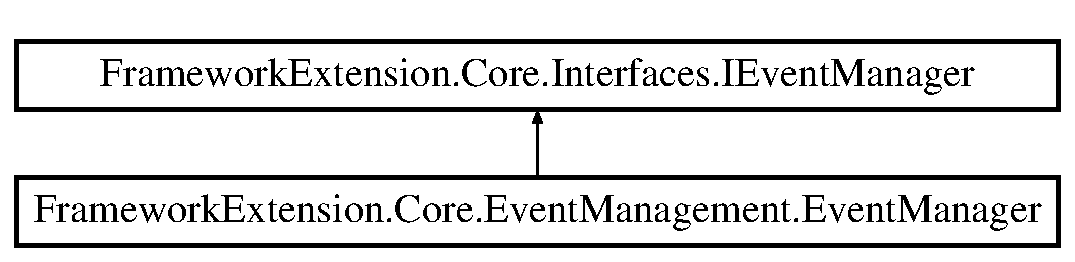
\includegraphics[height=2.000000cm]{interface_framework_extension_1_1_core_1_1_interfaces_1_1_i_event_manager}
\end{center}
\end{figure}
\subsection*{Public Member Functions}
\begin{DoxyCompactItemize}
\item 
\hypertarget{interface_framework_extension_1_1_core_1_1_interfaces_1_1_i_event_manager_a5c408030a49298d8f6347c4445fe8240}{void {\bfseries Register$<$ T $>$} (\hyperlink{interface_framework_extension_1_1_core_1_1_interfaces_1_1_i_interceptor-g}{I\-Interceptor}$<$ T $>$ interceptor)}\label{interface_framework_extension_1_1_core_1_1_interfaces_1_1_i_event_manager_a5c408030a49298d8f6347c4445fe8240}

\end{DoxyCompactItemize}
\subsection*{Properties}
\begin{DoxyCompactItemize}
\item 
\hypertarget{interface_framework_extension_1_1_core_1_1_interfaces_1_1_i_event_manager_a8f8e636145ede1602c51468a189548a3}{\hyperlink{interface_framework_extension_1_1_core_1_1_interfaces_1_1_i_observable_data_context}{I\-Observable\-Data\-Context} {\bfseries Context}\hspace{0.3cm}{\ttfamily  \mbox{[}get, set\mbox{]}}}\label{interface_framework_extension_1_1_core_1_1_interfaces_1_1_i_event_manager_a8f8e636145ede1602c51468a189548a3}

\end{DoxyCompactItemize}


The documentation for this interface was generated from the following file\-:\begin{DoxyCompactItemize}
\item 
Framework\-Extension.\-Core/\-Interfaces/I\-Event\-Manager.\-cs\end{DoxyCompactItemize}

\hypertarget{interface_framework_extension_1_1_core_1_1_interfaces_1_1_i_extendable_query}{\section{Framework\-Extension.\-Core.\-Interfaces.\-I\-Extendable\-Query Interface Reference}
\label{interface_framework_extension_1_1_core_1_1_interfaces_1_1_i_extendable_query}\index{Framework\-Extension.\-Core.\-Interfaces.\-I\-Extendable\-Query@{Framework\-Extension.\-Core.\-Interfaces.\-I\-Extendable\-Query}}
}
Inheritance diagram for Framework\-Extension.\-Core.\-Interfaces.\-I\-Extendable\-Query\-:\begin{figure}[H]
\begin{center}
\leavevmode
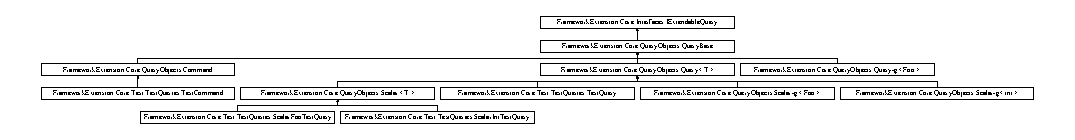
\includegraphics[height=1.435897cm]{interface_framework_extension_1_1_core_1_1_interfaces_1_1_i_extendable_query}
\end{center}
\end{figure}
\subsection*{Public Member Functions}
\begin{DoxyCompactItemize}
\item 
\hypertarget{interface_framework_extension_1_1_core_1_1_interfaces_1_1_i_extendable_query_ad95cd62b9f8cc132afd44759f849b9a1}{void {\bfseries Add\-Method\-Expression} (string method\-Name, Type\mbox{[}$\,$\mbox{]} generics, Expression\mbox{[}$\,$\mbox{]} parameters)}\label{interface_framework_extension_1_1_core_1_1_interfaces_1_1_i_extendable_query_ad95cd62b9f8cc132afd44759f849b9a1}

\end{DoxyCompactItemize}


The documentation for this interface was generated from the following file\-:\begin{DoxyCompactItemize}
\item 
Framework\-Extension.\-Core/\-Interfaces/I\-Extendable\-Query.\-cs\end{DoxyCompactItemize}

\hypertarget{interface_framework_extension_1_1_core_1_1_interfaces_1_1_i_interceptor-g}{\section{Framework\-Extension.\-Core.\-Interfaces.\-I\-Interceptor$<$ in T $>$ Interface Template Reference}
\label{interface_framework_extension_1_1_core_1_1_interfaces_1_1_i_interceptor-g}\index{Framework\-Extension.\-Core.\-Interfaces.\-I\-Interceptor$<$ in T $>$@{Framework\-Extension.\-Core.\-Interfaces.\-I\-Interceptor$<$ in T $>$}}
}
Inheritance diagram for Framework\-Extension.\-Core.\-Interfaces.\-I\-Interceptor$<$ in T $>$\-:\begin{figure}[H]
\begin{center}
\leavevmode
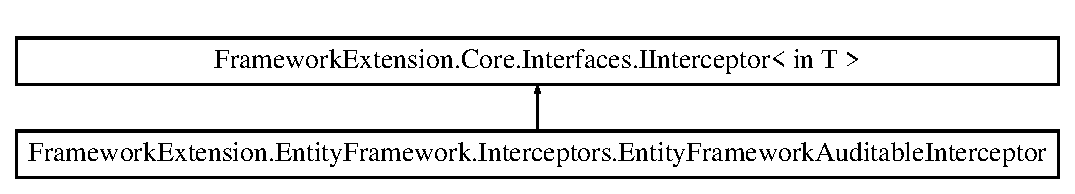
\includegraphics[height=2.000000cm]{interface_framework_extension_1_1_core_1_1_interfaces_1_1_i_interceptor-g}
\end{center}
\end{figure}
\subsection*{Public Member Functions}
\begin{DoxyCompactItemize}
\item 
\hypertarget{interface_framework_extension_1_1_core_1_1_interfaces_1_1_i_interceptor-g_a29390fc2dbc8566a239a46ce86431948}{\hyperlink{struct_framework_extension_1_1_core_1_1_interceptors_1_1_interceptor_result}{Interceptor\-Result} {\bfseries Execute} (\hyperlink{interface_framework_extension_1_1_core_1_1_interfaces_1_1_i_data_context}{I\-Data\-Context} context, T event\-Args)}\label{interface_framework_extension_1_1_core_1_1_interfaces_1_1_i_interceptor-g_a29390fc2dbc8566a239a46ce86431948}

\end{DoxyCompactItemize}
\subsection*{Properties}
\begin{DoxyCompactItemize}
\item 
\hypertarget{interface_framework_extension_1_1_core_1_1_interfaces_1_1_i_interceptor-g_a8dad5bbb0d6784578d68e58e8d836f2c}{int {\bfseries Priority}\hspace{0.3cm}{\ttfamily  \mbox{[}get, set\mbox{]}}}\label{interface_framework_extension_1_1_core_1_1_interfaces_1_1_i_interceptor-g_a8dad5bbb0d6784578d68e58e8d836f2c}

\end{DoxyCompactItemize}


The documentation for this interface was generated from the following file\-:\begin{DoxyCompactItemize}
\item 
Framework\-Extension.\-Core/\-Interfaces/I\-Interceptor.\-cs\end{DoxyCompactItemize}

\hypertarget{interface_framework_extension_1_1_entity_framework_1_1_mappings_1_1_i_mapping_configuration}{\section{Framework\-Extension.\-Entity\-Framework.\-Mappings.\-I\-Mapping\-Configuration Interface Reference}
\label{interface_framework_extension_1_1_entity_framework_1_1_mappings_1_1_i_mapping_configuration}\index{Framework\-Extension.\-Entity\-Framework.\-Mappings.\-I\-Mapping\-Configuration@{Framework\-Extension.\-Entity\-Framework.\-Mappings.\-I\-Mapping\-Configuration}}
}


Implement this interface to pass the mappings in via constructor injection on the context.  


Inheritance diagram for Framework\-Extension.\-Entity\-Framework.\-Mappings.\-I\-Mapping\-Configuration\-:\begin{figure}[H]
\begin{center}
\leavevmode
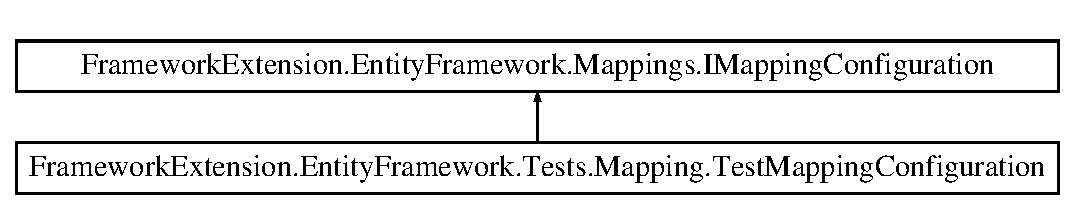
\includegraphics[height=2.000000cm]{interface_framework_extension_1_1_entity_framework_1_1_mappings_1_1_i_mapping_configuration}
\end{center}
\end{figure}
\subsection*{Public Member Functions}
\begin{DoxyCompactItemize}
\item 
void \hyperlink{interface_framework_extension_1_1_entity_framework_1_1_mappings_1_1_i_mapping_configuration_a4c3e96e66c2a5c926b2cf6d60d7289a6}{Configure\-Model\-Builder} (Db\-Model\-Builder model\-Builder)
\begin{DoxyCompactList}\small\item\em This method takes the model\-Builder from Entity Framework and wires in the mappings provided \end{DoxyCompactList}\end{DoxyCompactItemize}


\subsection{Detailed Description}
Implement this interface to pass the mappings in via constructor injection on the context. 



\subsection{Member Function Documentation}
\hypertarget{interface_framework_extension_1_1_entity_framework_1_1_mappings_1_1_i_mapping_configuration_a4c3e96e66c2a5c926b2cf6d60d7289a6}{\index{Framework\-Extension\-::\-Entity\-Framework\-::\-Mappings\-::\-I\-Mapping\-Configuration@{Framework\-Extension\-::\-Entity\-Framework\-::\-Mappings\-::\-I\-Mapping\-Configuration}!Configure\-Model\-Builder@{Configure\-Model\-Builder}}
\index{Configure\-Model\-Builder@{Configure\-Model\-Builder}!FrameworkExtension::EntityFramework::Mappings::IMappingConfiguration@{Framework\-Extension\-::\-Entity\-Framework\-::\-Mappings\-::\-I\-Mapping\-Configuration}}
\subsubsection[{Configure\-Model\-Builder}]{\setlength{\rightskip}{0pt plus 5cm}void Framework\-Extension.\-Entity\-Framework.\-Mappings.\-I\-Mapping\-Configuration.\-Configure\-Model\-Builder (
\begin{DoxyParamCaption}
\item[{Db\-Model\-Builder}]{model\-Builder}
\end{DoxyParamCaption}
)}}\label{interface_framework_extension_1_1_entity_framework_1_1_mappings_1_1_i_mapping_configuration_a4c3e96e66c2a5c926b2cf6d60d7289a6}


This method takes the model\-Builder from Entity Framework and wires in the mappings provided 


\begin{DoxyParams}{Parameters}
{\em model\-Builder} & The Database model builder used by Entity Framework to generate the model.\\
\hline
\end{DoxyParams}


Implemented in \hyperlink{class_framework_extension_1_1_entity_framework_1_1_tests_1_1_mapping_1_1_test_mapping_configuration_ab3e0ed1691f37fa30871356ba49f88eb}{Framework\-Extension.\-Entity\-Framework.\-Tests.\-Mapping.\-Test\-Mapping\-Configuration}.



The documentation for this interface was generated from the following file\-:\begin{DoxyCompactItemize}
\item 
Framework\-Extension.\-Entity\-Framework/\-Mappings/I\-Mapping\-Configuration.\-cs\end{DoxyCompactItemize}

\hypertarget{struct_framework_extension_1_1_core_1_1_interceptors_1_1_interceptor_result}{\section{Framework\-Extension.\-Core.\-Interceptors.\-Interceptor\-Result Struct Reference}
\label{struct_framework_extension_1_1_core_1_1_interceptors_1_1_interceptor_result}\index{Framework\-Extension.\-Core.\-Interceptors.\-Interceptor\-Result@{Framework\-Extension.\-Core.\-Interceptors.\-Interceptor\-Result}}
}
\subsection*{Static Public Member Functions}
\begin{DoxyCompactItemize}
\item 
\hypertarget{struct_framework_extension_1_1_core_1_1_interceptors_1_1_interceptor_result_aad16e0d9771fab36488d440f4ddc4102}{static \hyperlink{struct_framework_extension_1_1_core_1_1_interceptors_1_1_interceptor_result}{Interceptor\-Result} {\bfseries Succeeded} ()}\label{struct_framework_extension_1_1_core_1_1_interceptors_1_1_interceptor_result_aad16e0d9771fab36488d440f4ddc4102}

\item 
\hypertarget{struct_framework_extension_1_1_core_1_1_interceptors_1_1_interceptor_result_a294a218afdce7ba0ff6849a851f45c4d}{static \hyperlink{struct_framework_extension_1_1_core_1_1_interceptors_1_1_interceptor_result}{Interceptor\-Result} {\bfseries Failed} (string message, bool continue\-To\-Execute=false)}\label{struct_framework_extension_1_1_core_1_1_interceptors_1_1_interceptor_result_a294a218afdce7ba0ff6849a851f45c4d}

\end{DoxyCompactItemize}
\subsection*{Properties}
\begin{DoxyCompactItemize}
\item 
\hypertarget{struct_framework_extension_1_1_core_1_1_interceptors_1_1_interceptor_result_a1fc3c9b79351c287b4daf4887f41f3fe}{bool {\bfseries Continue\-Execution}\hspace{0.3cm}{\ttfamily  \mbox{[}get, set\mbox{]}}}\label{struct_framework_extension_1_1_core_1_1_interceptors_1_1_interceptor_result_a1fc3c9b79351c287b4daf4887f41f3fe}

\item 
\hypertarget{struct_framework_extension_1_1_core_1_1_interceptors_1_1_interceptor_result_a9a282901dd73c684539ccedd518ee6f4}{string {\bfseries Message}\hspace{0.3cm}{\ttfamily  \mbox{[}get, set\mbox{]}}}\label{struct_framework_extension_1_1_core_1_1_interceptors_1_1_interceptor_result_a9a282901dd73c684539ccedd518ee6f4}

\end{DoxyCompactItemize}


The documentation for this struct was generated from the following file\-:\begin{DoxyCompactItemize}
\item 
Framework\-Extension.\-Core/\-Interceptors/Interceptor\-Result.\-cs\end{DoxyCompactItemize}

\hypertarget{interface_framework_extension_1_1_core_1_1_interfaces_1_1_i_observable_data_context}{\section{Framework\-Extension.\-Core.\-Interfaces.\-I\-Observable\-Data\-Context Interface Reference}
\label{interface_framework_extension_1_1_core_1_1_interfaces_1_1_i_observable_data_context}\index{Framework\-Extension.\-Core.\-Interfaces.\-I\-Observable\-Data\-Context@{Framework\-Extension.\-Core.\-Interfaces.\-I\-Observable\-Data\-Context}}
}
Inheritance diagram for Framework\-Extension.\-Core.\-Interfaces.\-I\-Observable\-Data\-Context\-:\begin{figure}[H]
\begin{center}
\leavevmode
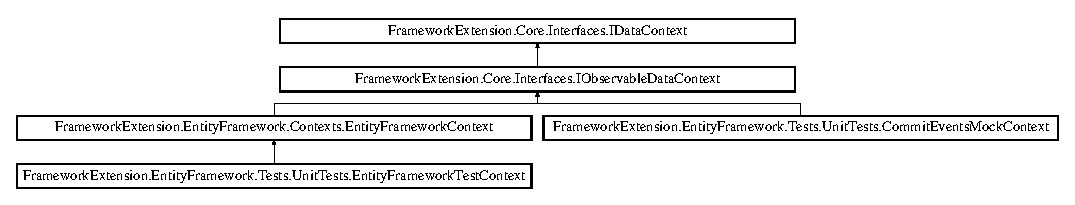
\includegraphics[height=2.309278cm]{interface_framework_extension_1_1_core_1_1_interfaces_1_1_i_observable_data_context}
\end{center}
\end{figure}
\subsection*{Events}
\begin{DoxyCompactItemize}
\item 
\hypertarget{interface_framework_extension_1_1_core_1_1_interfaces_1_1_i_observable_data_context_a1639996a55aaeb6001c8044561e1b3e3}{Event\-Handler$<$ \hyperlink{class_framework_extension_1_1_core_1_1_interceptors_1_1_events_1_1_pre_save_event_args}{Pre\-Save\-Event\-Args} $>$ {\bfseries Pre\-Save}}\label{interface_framework_extension_1_1_core_1_1_interfaces_1_1_i_observable_data_context_a1639996a55aaeb6001c8044561e1b3e3}

\item 
\hypertarget{interface_framework_extension_1_1_core_1_1_interfaces_1_1_i_observable_data_context_aee463e57933af818ce34fab005fbff96}{Event\-Handler$<$ \hyperlink{class_framework_extension_1_1_core_1_1_interceptors_1_1_events_1_1_post_save_event_args}{Post\-Save\-Event\-Args} $>$ {\bfseries Post\-Save}}\label{interface_framework_extension_1_1_core_1_1_interfaces_1_1_i_observable_data_context_aee463e57933af818ce34fab005fbff96}

\end{DoxyCompactItemize}
\subsection*{Additional Inherited Members}


The documentation for this interface was generated from the following file\-:\begin{DoxyCompactItemize}
\item 
Framework\-Extension.\-Core/\-Interfaces/I\-Observable\-Data\-Context.\-cs\end{DoxyCompactItemize}

\hypertarget{class_i_query-g}{\section{I\-Query Class Reference}
\label{class_i_query-g}\index{I\-Query@{I\-Query}}
}
Inheritance diagram for I\-Query\-:\begin{figure}[H]
\begin{center}
\leavevmode
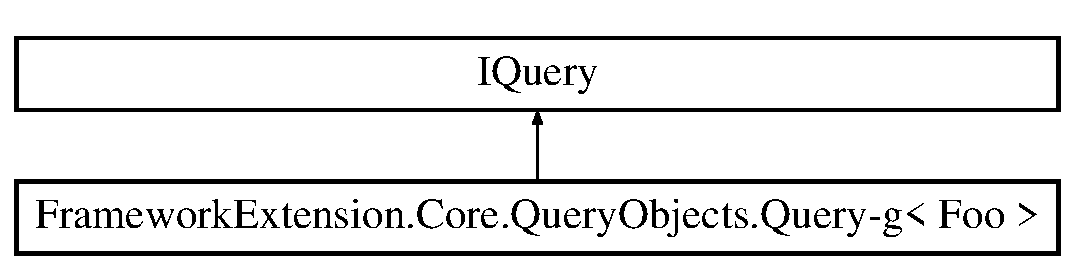
\includegraphics[height=2.000000cm]{class_i_query-g}
\end{center}
\end{figure}


The documentation for this class was generated from the following file\-:\begin{DoxyCompactItemize}
\item 
Highway.\-Data/\-Query\-Objects/Query.\-cs\end{DoxyCompactItemize}

\hypertarget{interface_framework_extension_1_1_core_1_1_interfaces_1_1_i_query-g}{\section{Framework\-Extension.\-Core.\-Interfaces.\-I\-Query$<$ out T $>$ Interface Template Reference}
\label{interface_framework_extension_1_1_core_1_1_interfaces_1_1_i_query-g}\index{Framework\-Extension.\-Core.\-Interfaces.\-I\-Query$<$ out T $>$@{Framework\-Extension.\-Core.\-Interfaces.\-I\-Query$<$ out T $>$}}
}
Inheritance diagram for Framework\-Extension.\-Core.\-Interfaces.\-I\-Query$<$ out T $>$\-:\begin{figure}[H]
\begin{center}
\leavevmode
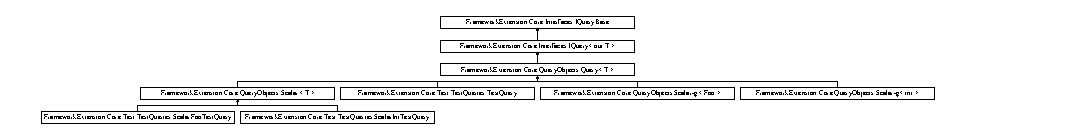
\includegraphics[height=1.435897cm]{interface_framework_extension_1_1_core_1_1_interfaces_1_1_i_query-g}
\end{center}
\end{figure}
\subsection*{Public Member Functions}
\begin{DoxyCompactItemize}
\item 
I\-Enumerable$<$ T $>$ \hyperlink{interface_framework_extension_1_1_core_1_1_interfaces_1_1_i_query-g_aeadee7cdb945427ce105b13caa124969}{Execute} (\hyperlink{interface_framework_extension_1_1_core_1_1_interfaces_1_1_i_data_context}{I\-Data\-Context} context)
\begin{DoxyCompactList}\small\item\em This executes the expression in Context\-Query on the context that is passed in, resulting in a I\-Queryable
\begin{DoxyTemplParams}{Template Parameters}
{\em T} & \\
\hline
\end{DoxyTemplParams}
that is returned as an I\-Enumerable
\begin{DoxyTemplParams}{Template Parameters}
{\em T} & \\
\hline
\end{DoxyTemplParams}
\end{DoxyCompactList}\end{DoxyCompactItemize}


\subsection{Member Function Documentation}
\hypertarget{interface_framework_extension_1_1_core_1_1_interfaces_1_1_i_query-g_aeadee7cdb945427ce105b13caa124969}{\index{Framework\-Extension\-::\-Core\-::\-Interfaces\-::\-I\-Query-\/g@{Framework\-Extension\-::\-Core\-::\-Interfaces\-::\-I\-Query-\/g}!Execute@{Execute}}
\index{Execute@{Execute}!FrameworkExtension::Core::Interfaces::IQuery-g@{Framework\-Extension\-::\-Core\-::\-Interfaces\-::\-I\-Query-\/g}}
\subsubsection[{Execute}]{\setlength{\rightskip}{0pt plus 5cm}template$<$out T$>$ I\-Enumerable$<$T$>$ {\bf Framework\-Extension.\-Core.\-Interfaces.\-I\-Query}$<$ out T $>$.Execute (
\begin{DoxyParamCaption}
\item[{{\bf I\-Data\-Context}}]{context}
\end{DoxyParamCaption}
)}}\label{interface_framework_extension_1_1_core_1_1_interfaces_1_1_i_query-g_aeadee7cdb945427ce105b13caa124969}


This executes the expression in Context\-Query on the context that is passed in, resulting in a I\-Queryable
\begin{DoxyTemplParams}{Template Parameters}
{\em T} & \\
\hline
\end{DoxyTemplParams}
that is returned as an I\-Enumerable
\begin{DoxyTemplParams}{Template Parameters}
{\em T} & \\
\hline
\end{DoxyTemplParams}



\begin{DoxyParams}{Parameters}
{\em context} & the data context that the query should be executed against\\
\hline
\end{DoxyParams}
\begin{DoxyReturn}{Returns}
I\-Enumerable
\begin{DoxyTemplParams}{Template Parameters}
{\em T} & \\
\hline
\end{DoxyTemplParams}

\end{DoxyReturn}


Implemented in \hyperlink{class_framework_extension_1_1_core_1_1_query_objects_1_1_query-g_a492abefd04cb45983c1ac76c4ae4acb7}{Framework\-Extension.\-Core.\-Query\-Objects.\-Query$<$ T $>$}.



The documentation for this interface was generated from the following file\-:\begin{DoxyCompactItemize}
\item 
Framework\-Extension.\-Core/\-Interfaces/I\-Query.\-cs\end{DoxyCompactItemize}

\hypertarget{interface_framework_extension_1_1_core_1_1_interfaces_1_1_i_query_base}{\section{Framework\-Extension.\-Core.\-Interfaces.\-I\-Query\-Base Interface Reference}
\label{interface_framework_extension_1_1_core_1_1_interfaces_1_1_i_query_base}\index{Framework\-Extension.\-Core.\-Interfaces.\-I\-Query\-Base@{Framework\-Extension.\-Core.\-Interfaces.\-I\-Query\-Base}}
}
Inheritance diagram for Framework\-Extension.\-Core.\-Interfaces.\-I\-Query\-Base\-:\begin{figure}[H]
\begin{center}
\leavevmode
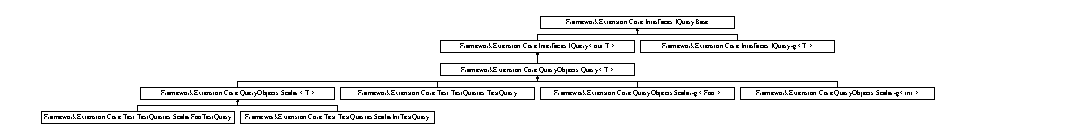
\includegraphics[height=1.435897cm]{interface_framework_extension_1_1_core_1_1_interfaces_1_1_i_query_base}
\end{center}
\end{figure}
\subsection*{Public Member Functions}
\begin{DoxyCompactItemize}
\item 
string \hyperlink{interface_framework_extension_1_1_core_1_1_interfaces_1_1_i_query_base_accf6af70d0aea2df1721e910e9217f48}{Output\-S\-Q\-L\-Statement} (\hyperlink{interface_framework_extension_1_1_core_1_1_interfaces_1_1_i_data_context}{I\-Data\-Context} context)
\begin{DoxyCompactList}\small\item\em This executes the expression against the passed in context to generate the S\-Q\-L statement, but doesn't execute the I\-Queryable
\begin{DoxyTemplParams}{Template Parameters}
{\em T} & \\
\hline
\end{DoxyTemplParams}
against the data context \end{DoxyCompactList}\end{DoxyCompactItemize}


\subsection{Member Function Documentation}
\hypertarget{interface_framework_extension_1_1_core_1_1_interfaces_1_1_i_query_base_accf6af70d0aea2df1721e910e9217f48}{\index{Framework\-Extension\-::\-Core\-::\-Interfaces\-::\-I\-Query\-Base@{Framework\-Extension\-::\-Core\-::\-Interfaces\-::\-I\-Query\-Base}!Output\-S\-Q\-L\-Statement@{Output\-S\-Q\-L\-Statement}}
\index{Output\-S\-Q\-L\-Statement@{Output\-S\-Q\-L\-Statement}!FrameworkExtension::Core::Interfaces::IQueryBase@{Framework\-Extension\-::\-Core\-::\-Interfaces\-::\-I\-Query\-Base}}
\subsubsection[{Output\-S\-Q\-L\-Statement}]{\setlength{\rightskip}{0pt plus 5cm}string Framework\-Extension.\-Core.\-Interfaces.\-I\-Query\-Base.\-Output\-S\-Q\-L\-Statement (
\begin{DoxyParamCaption}
\item[{{\bf I\-Data\-Context}}]{context}
\end{DoxyParamCaption}
)}}\label{interface_framework_extension_1_1_core_1_1_interfaces_1_1_i_query_base_accf6af70d0aea2df1721e910e9217f48}


This executes the expression against the passed in context to generate the S\-Q\-L statement, but doesn't execute the I\-Queryable
\begin{DoxyTemplParams}{Template Parameters}
{\em T} & \\
\hline
\end{DoxyTemplParams}
against the data context 


\begin{DoxyParams}{Parameters}
{\em context} & The data context that the query is evaluated and the S\-Q\-L is generated against\\
\hline
\end{DoxyParams}
\begin{DoxyReturn}{Returns}
The S\-Q\-L Statement from the Query
\end{DoxyReturn}


Implemented in \hyperlink{class_framework_extension_1_1_core_1_1_query_objects_1_1_query-g_af5d93ae2f7a467a48500683857b842d2}{Framework\-Extension.\-Core.\-Query\-Objects.\-Query$<$ T $>$}.



The documentation for this interface was generated from the following file\-:\begin{DoxyCompactItemize}
\item 
Framework\-Extension.\-Core/\-Interfaces/I\-Query.\-cs\end{DoxyCompactItemize}

\hypertarget{interface_framework_extension_1_1_core_1_1_interfaces_1_1_i_repository}{\section{Framework\-Extension.\-Core.\-Interfaces.\-I\-Repository Interface Reference}
\label{interface_framework_extension_1_1_core_1_1_interfaces_1_1_i_repository}\index{Framework\-Extension.\-Core.\-Interfaces.\-I\-Repository@{Framework\-Extension.\-Core.\-Interfaces.\-I\-Repository}}
}
Inheritance diagram for Framework\-Extension.\-Core.\-Interfaces.\-I\-Repository\-:\begin{figure}[H]
\begin{center}
\leavevmode
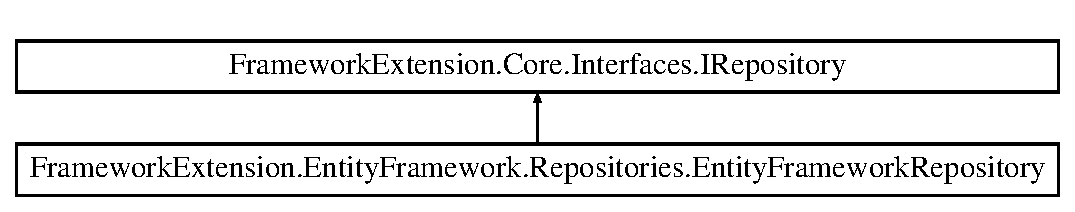
\includegraphics[height=2.000000cm]{interface_framework_extension_1_1_core_1_1_interfaces_1_1_i_repository}
\end{center}
\end{figure}
\subsection*{Public Member Functions}
\begin{DoxyCompactItemize}
\item 
\hypertarget{interface_framework_extension_1_1_core_1_1_interfaces_1_1_i_repository_ade00c49cbf4c15c6fcd358266f91d507}{I\-Enumerable$<$ T $>$ {\bfseries Find$<$ T $>$} (\hyperlink{interface_framework_extension_1_1_core_1_1_interfaces_1_1_i_query-g}{I\-Query}$<$ T $>$ query)}\label{interface_framework_extension_1_1_core_1_1_interfaces_1_1_i_repository_ade00c49cbf4c15c6fcd358266f91d507}

\item 
\hypertarget{interface_framework_extension_1_1_core_1_1_interfaces_1_1_i_repository_aee59bce54af0de81a434a54e2726aa85}{T {\bfseries Get$<$ T $>$} (\hyperlink{interface_framework_extension_1_1_core_1_1_interfaces_1_1_i_scalar_object-g}{I\-Scalar\-Object}$<$ T $>$ query)}\label{interface_framework_extension_1_1_core_1_1_interfaces_1_1_i_repository_aee59bce54af0de81a434a54e2726aa85}

\item 
\hypertarget{interface_framework_extension_1_1_core_1_1_interfaces_1_1_i_repository_a75a06316c9cb660a2a3fa8d1d2156e9b}{void {\bfseries Execute} (\hyperlink{interface_framework_extension_1_1_core_1_1_interfaces_1_1_i_command_object}{I\-Command\-Object} command)}\label{interface_framework_extension_1_1_core_1_1_interfaces_1_1_i_repository_a75a06316c9cb660a2a3fa8d1d2156e9b}

\end{DoxyCompactItemize}
\subsection*{Properties}
\begin{DoxyCompactItemize}
\item 
\hypertarget{interface_framework_extension_1_1_core_1_1_interfaces_1_1_i_repository_a20857c9d0e76f5a1036622c24c57f46d}{\hyperlink{interface_framework_extension_1_1_core_1_1_interfaces_1_1_i_data_context}{I\-Data\-Context} {\bfseries Context}\hspace{0.3cm}{\ttfamily  \mbox{[}get\mbox{]}}}\label{interface_framework_extension_1_1_core_1_1_interfaces_1_1_i_repository_a20857c9d0e76f5a1036622c24c57f46d}

\item 
\hypertarget{interface_framework_extension_1_1_core_1_1_interfaces_1_1_i_repository_a93f60b836e59eb79ba13b5384b17bb19}{\hyperlink{interface_framework_extension_1_1_core_1_1_interfaces_1_1_i_event_manager}{I\-Event\-Manager} {\bfseries Event\-Manager}\hspace{0.3cm}{\ttfamily  \mbox{[}get\mbox{]}}}\label{interface_framework_extension_1_1_core_1_1_interfaces_1_1_i_repository_a93f60b836e59eb79ba13b5384b17bb19}

\end{DoxyCompactItemize}


The documentation for this interface was generated from the following file\-:\begin{DoxyCompactItemize}
\item 
Framework\-Extension.\-Core/\-Interfaces/I\-Repository.\-cs\end{DoxyCompactItemize}

\hypertarget{class_i_scalar_object-g}{\section{I\-Scalar\-Object Class Reference}
\label{class_i_scalar_object-g}\index{I\-Scalar\-Object@{I\-Scalar\-Object}}
}
Inheritance diagram for I\-Scalar\-Object\-:\begin{figure}[H]
\begin{center}
\leavevmode
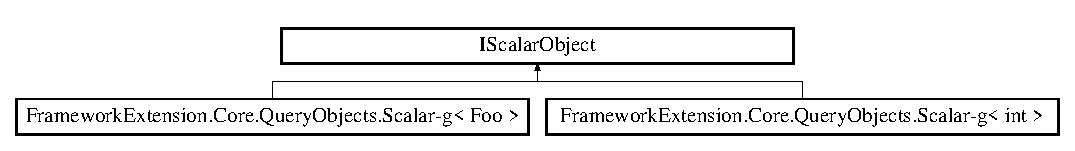
\includegraphics[height=1.978799cm]{class_i_scalar_object-g}
\end{center}
\end{figure}


The documentation for this class was generated from the following file\-:\begin{DoxyCompactItemize}
\item 
Highway.\-Data/\-Query\-Objects/Scalar.\-cs\end{DoxyCompactItemize}

\hypertarget{interface_framework_extension_1_1_core_1_1_interfaces_1_1_i_scalar_object-g}{\section{Framework\-Extension.\-Core.\-Interfaces.\-I\-Scalar\-Object$<$ out T $>$ Interface Template Reference}
\label{interface_framework_extension_1_1_core_1_1_interfaces_1_1_i_scalar_object-g}\index{Framework\-Extension.\-Core.\-Interfaces.\-I\-Scalar\-Object$<$ out T $>$@{Framework\-Extension.\-Core.\-Interfaces.\-I\-Scalar\-Object$<$ out T $>$}}
}
Inheritance diagram for Framework\-Extension.\-Core.\-Interfaces.\-I\-Scalar\-Object$<$ out T $>$\-:\begin{figure}[H]
\begin{center}
\leavevmode
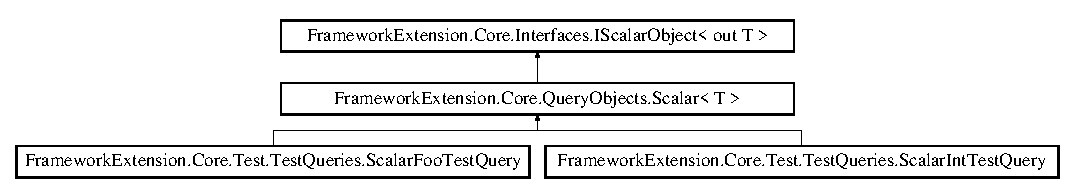
\includegraphics[height=2.153846cm]{interface_framework_extension_1_1_core_1_1_interfaces_1_1_i_scalar_object-g}
\end{center}
\end{figure}
\subsection*{Public Member Functions}
\begin{DoxyCompactItemize}
\item 
\hypertarget{interface_framework_extension_1_1_core_1_1_interfaces_1_1_i_scalar_object-g_a1ea51f0b87546fa95ae792a6c23663e5}{T {\bfseries Execute} (\hyperlink{interface_framework_extension_1_1_core_1_1_interfaces_1_1_i_data_context}{I\-Data\-Context} context)}\label{interface_framework_extension_1_1_core_1_1_interfaces_1_1_i_scalar_object-g_a1ea51f0b87546fa95ae792a6c23663e5}

\end{DoxyCompactItemize}


The documentation for this interface was generated from the following file\-:\begin{DoxyCompactItemize}
\item 
Framework\-Extension.\-Core/\-Interfaces/I\-Query.\-cs\end{DoxyCompactItemize}

\hypertarget{interface_framework_extension_1_1_core_1_1_interfaces_1_1_i_user_name_service}{\section{Framework\-Extension.\-Core.\-Interfaces.\-I\-User\-Name\-Service Interface Reference}
\label{interface_framework_extension_1_1_core_1_1_interfaces_1_1_i_user_name_service}\index{Framework\-Extension.\-Core.\-Interfaces.\-I\-User\-Name\-Service@{Framework\-Extension.\-Core.\-Interfaces.\-I\-User\-Name\-Service}}
}
Inheritance diagram for Framework\-Extension.\-Core.\-Interfaces.\-I\-User\-Name\-Service\-:\begin{figure}[H]
\begin{center}
\leavevmode
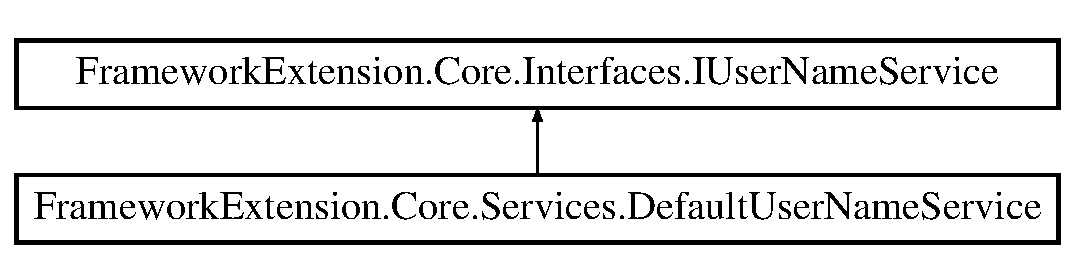
\includegraphics[height=2.000000cm]{interface_framework_extension_1_1_core_1_1_interfaces_1_1_i_user_name_service}
\end{center}
\end{figure}
\subsection*{Public Member Functions}
\begin{DoxyCompactItemize}
\item 
\hypertarget{interface_framework_extension_1_1_core_1_1_interfaces_1_1_i_user_name_service_a6812cf2daf0585c264219dd4354283ce}{string {\bfseries Get\-Current\-User\-Name} ()}\label{interface_framework_extension_1_1_core_1_1_interfaces_1_1_i_user_name_service_a6812cf2daf0585c264219dd4354283ce}

\end{DoxyCompactItemize}


The documentation for this interface was generated from the following file\-:\begin{DoxyCompactItemize}
\item 
Framework\-Extension.\-Core/\-Interfaces/I\-User\-Name\-Service.\-cs\end{DoxyCompactItemize}

\hypertarget{class_framework_extension_1_1_core_1_1_interceptors_1_1_events_1_1_post_query_event_args}{\section{Framework\-Extension.\-Core.\-Interceptors.\-Events.\-Post\-Query\-Event\-Args Class Reference}
\label{class_framework_extension_1_1_core_1_1_interceptors_1_1_events_1_1_post_query_event_args}\index{Framework\-Extension.\-Core.\-Interceptors.\-Events.\-Post\-Query\-Event\-Args@{Framework\-Extension.\-Core.\-Interceptors.\-Events.\-Post\-Query\-Event\-Args}}
}


The documentation for this class was generated from the following file\-:\begin{DoxyCompactItemize}
\item 
Framework\-Extension.\-Core/\-Interceptors/\-Events/Post\-Query\-Event\-Args.\-cs\end{DoxyCompactItemize}

\hypertarget{class_framework_extension_1_1_core_1_1_interceptors_1_1_events_1_1_post_save_event_args}{\section{Framework\-Extension.\-Core.\-Interceptors.\-Events.\-Post\-Save\-Event\-Args Class Reference}
\label{class_framework_extension_1_1_core_1_1_interceptors_1_1_events_1_1_post_save_event_args}\index{Framework\-Extension.\-Core.\-Interceptors.\-Events.\-Post\-Save\-Event\-Args@{Framework\-Extension.\-Core.\-Interceptors.\-Events.\-Post\-Save\-Event\-Args}}
}


The documentation for this class was generated from the following file\-:\begin{DoxyCompactItemize}
\item 
Framework\-Extension.\-Core/\-Interceptors/\-Events/Post\-Save\-Event\-Args.\-cs\end{DoxyCompactItemize}

\hypertarget{class_framework_extension_1_1_core_1_1_interceptors_1_1_events_1_1_pre_query_event_args}{\section{Framework\-Extension.\-Core.\-Interceptors.\-Events.\-Pre\-Query\-Event\-Args Class Reference}
\label{class_framework_extension_1_1_core_1_1_interceptors_1_1_events_1_1_pre_query_event_args}\index{Framework\-Extension.\-Core.\-Interceptors.\-Events.\-Pre\-Query\-Event\-Args@{Framework\-Extension.\-Core.\-Interceptors.\-Events.\-Pre\-Query\-Event\-Args}}
}


The documentation for this class was generated from the following file\-:\begin{DoxyCompactItemize}
\item 
Framework\-Extension.\-Core/\-Interceptors/\-Events/Pre\-Query\-Event\-Args.\-cs\end{DoxyCompactItemize}

\hypertarget{class_framework_extension_1_1_core_1_1_interceptors_1_1_events_1_1_pre_save_event_args}{\section{Framework\-Extension.\-Core.\-Interceptors.\-Events.\-Pre\-Save\-Event\-Args Class Reference}
\label{class_framework_extension_1_1_core_1_1_interceptors_1_1_events_1_1_pre_save_event_args}\index{Framework\-Extension.\-Core.\-Interceptors.\-Events.\-Pre\-Save\-Event\-Args@{Framework\-Extension.\-Core.\-Interceptors.\-Events.\-Pre\-Save\-Event\-Args}}
}


The documentation for this class was generated from the following file\-:\begin{DoxyCompactItemize}
\item 
Framework\-Extension.\-Core/\-Interceptors/\-Events/Pre\-Save\-Event\-Args.\-cs\end{DoxyCompactItemize}

\hypertarget{class_framework_extension_1_1_core_1_1_query_objects_1_1_query-g}{\section{Framework\-Extension.\-Core.\-Query\-Objects.\-Query$<$ T $>$ Class Template Reference}
\label{class_framework_extension_1_1_core_1_1_query_objects_1_1_query-g}\index{Framework\-Extension.\-Core.\-Query\-Objects.\-Query$<$ T $>$@{Framework\-Extension.\-Core.\-Query\-Objects.\-Query$<$ T $>$}}
}
Inheritance diagram for Framework\-Extension.\-Core.\-Query\-Objects.\-Query$<$ T $>$\-:\begin{figure}[H]
\begin{center}
\leavevmode
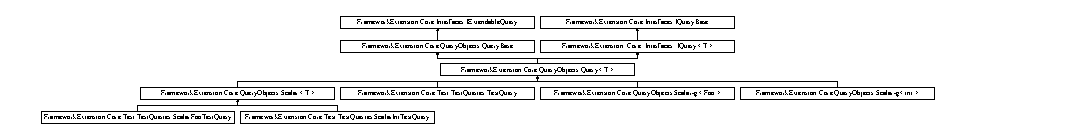
\includegraphics[height=1.435897cm]{class_framework_extension_1_1_core_1_1_query_objects_1_1_query-g}
\end{center}
\end{figure}
\subsection*{Public Member Functions}
\begin{DoxyCompactItemize}
\item 
virtual I\-Enumerable$<$ T $>$ \hyperlink{class_framework_extension_1_1_core_1_1_query_objects_1_1_query-g_a492abefd04cb45983c1ac76c4ae4acb7}{Execute} (\hyperlink{interface_framework_extension_1_1_core_1_1_interfaces_1_1_i_data_context}{I\-Data\-Context} context)
\begin{DoxyCompactList}\small\item\em This executes the expression in Context\-Query on the context that is passed in, resulting in a I\-Queryable
\begin{DoxyTemplParams}{Template Parameters}
{\em T} & \\
\hline
\end{DoxyTemplParams}
that is returned as an I\-Enumerable
\begin{DoxyTemplParams}{Template Parameters}
{\em T} & \\
\hline
\end{DoxyTemplParams}
\end{DoxyCompactList}\item 
string \hyperlink{class_framework_extension_1_1_core_1_1_query_objects_1_1_query-g_af5d93ae2f7a467a48500683857b842d2}{Output\-S\-Q\-L\-Statement} (\hyperlink{interface_framework_extension_1_1_core_1_1_interfaces_1_1_i_data_context}{I\-Data\-Context} context)
\begin{DoxyCompactList}\small\item\em This executes the expression against the passed in context to generate the S\-Q\-L statement, but doesn't execute the I\-Queryable
\begin{DoxyTemplParams}{Template Parameters}
{\em T} & \\
\hline
\end{DoxyTemplParams}
against the data context \end{DoxyCompactList}\end{DoxyCompactItemize}
\subsection*{Protected Member Functions}
\begin{DoxyCompactItemize}
\item 
virtual I\-Queryable$<$ T $>$ \hyperlink{class_framework_extension_1_1_core_1_1_query_objects_1_1_query-g_ac3a35701978540f4bab19f1785bb883c}{Extend\-Query} ()
\begin{DoxyCompactList}\small\item\em This method allows for the extension of Ordering and Grouping on the prebuild \hyperlink{class_framework_extension_1_1_core_1_1_query_objects_1_1_query-g}{Query} \end{DoxyCompactList}\item 
\hypertarget{class_framework_extension_1_1_core_1_1_query_objects_1_1_query-g_a86dbe1ad637e2f996819c41364f2eb4c}{I\-Queryable$<$ T $>$ {\bfseries Append\-Expressions} (I\-Queryable$<$ T $>$ query)}\label{class_framework_extension_1_1_core_1_1_query_objects_1_1_query-g_a86dbe1ad637e2f996819c41364f2eb4c}

\end{DoxyCompactItemize}
\subsection*{Properties}
\begin{DoxyCompactItemize}
\item 
Func$<$ \hyperlink{interface_framework_extension_1_1_core_1_1_interfaces_1_1_i_data_context}{I\-Data\-Context}, I\-Queryable\\*
$<$ T $>$ $>$ \hyperlink{class_framework_extension_1_1_core_1_1_query_objects_1_1_query-g_afc262d00f1a554c09fe74d2079d5e4c7}{Context\-Query}\hspace{0.3cm}{\ttfamily  \mbox{[}get, set\mbox{]}}
\begin{DoxyCompactList}\small\item\em This holds the expression that will be used to create the I\-Queryable
\begin{DoxyTemplParams}{Template Parameters}
{\em T} & \\
\hline
\end{DoxyTemplParams}
when executed on the context \end{DoxyCompactList}\end{DoxyCompactItemize}
\subsection*{Additional Inherited Members}


\subsection{Member Function Documentation}
\hypertarget{class_framework_extension_1_1_core_1_1_query_objects_1_1_query-g_a492abefd04cb45983c1ac76c4ae4acb7}{\index{Framework\-Extension\-::\-Core\-::\-Query\-Objects\-::\-Query-\/g@{Framework\-Extension\-::\-Core\-::\-Query\-Objects\-::\-Query-\/g}!Execute@{Execute}}
\index{Execute@{Execute}!FrameworkExtension::Core::QueryObjects::Query-g@{Framework\-Extension\-::\-Core\-::\-Query\-Objects\-::\-Query-\/g}}
\subsubsection[{Execute}]{\setlength{\rightskip}{0pt plus 5cm}template$<$T $>$ virtual I\-Enumerable$<$T$>$ {\bf Framework\-Extension.\-Core.\-Query\-Objects.\-Query}$<$ T $>$.Execute (
\begin{DoxyParamCaption}
\item[{{\bf I\-Data\-Context}}]{context}
\end{DoxyParamCaption}
)\hspace{0.3cm}{\ttfamily [inline]}, {\ttfamily [virtual]}}}\label{class_framework_extension_1_1_core_1_1_query_objects_1_1_query-g_a492abefd04cb45983c1ac76c4ae4acb7}


This executes the expression in Context\-Query on the context that is passed in, resulting in a I\-Queryable
\begin{DoxyTemplParams}{Template Parameters}
{\em T} & \\
\hline
\end{DoxyTemplParams}
that is returned as an I\-Enumerable
\begin{DoxyTemplParams}{Template Parameters}
{\em T} & \\
\hline
\end{DoxyTemplParams}



\begin{DoxyParams}{Parameters}
{\em context} & the data context that the query should be executed against\\
\hline
\end{DoxyParams}
\begin{DoxyReturn}{Returns}
I\-Enumerable
\begin{DoxyTemplParams}{Template Parameters}
{\em T} & \\
\hline
\end{DoxyTemplParams}

\end{DoxyReturn}


Implements \hyperlink{interface_framework_extension_1_1_core_1_1_interfaces_1_1_i_query-g_aeadee7cdb945427ce105b13caa124969}{Framework\-Extension.\-Core.\-Interfaces.\-I\-Query$<$ out T $>$}.

\hypertarget{class_framework_extension_1_1_core_1_1_query_objects_1_1_query-g_ac3a35701978540f4bab19f1785bb883c}{\index{Framework\-Extension\-::\-Core\-::\-Query\-Objects\-::\-Query-\/g@{Framework\-Extension\-::\-Core\-::\-Query\-Objects\-::\-Query-\/g}!Extend\-Query@{Extend\-Query}}
\index{Extend\-Query@{Extend\-Query}!FrameworkExtension::Core::QueryObjects::Query-g@{Framework\-Extension\-::\-Core\-::\-Query\-Objects\-::\-Query-\/g}}
\subsubsection[{Extend\-Query}]{\setlength{\rightskip}{0pt plus 5cm}template$<$T $>$ virtual I\-Queryable$<$T$>$ {\bf Framework\-Extension.\-Core.\-Query\-Objects.\-Query}$<$ T $>$.Extend\-Query (
\begin{DoxyParamCaption}
{}
\end{DoxyParamCaption}
)\hspace{0.3cm}{\ttfamily [inline]}, {\ttfamily [protected]}, {\ttfamily [virtual]}}}\label{class_framework_extension_1_1_core_1_1_query_objects_1_1_query-g_ac3a35701978540f4bab19f1785bb883c}


This method allows for the extension of Ordering and Grouping on the prebuild \hyperlink{class_framework_extension_1_1_core_1_1_query_objects_1_1_query-g}{Query} 

\begin{DoxyReturn}{Returns}

\end{DoxyReturn}
\hypertarget{class_framework_extension_1_1_core_1_1_query_objects_1_1_query-g_af5d93ae2f7a467a48500683857b842d2}{\index{Framework\-Extension\-::\-Core\-::\-Query\-Objects\-::\-Query-\/g@{Framework\-Extension\-::\-Core\-::\-Query\-Objects\-::\-Query-\/g}!Output\-S\-Q\-L\-Statement@{Output\-S\-Q\-L\-Statement}}
\index{Output\-S\-Q\-L\-Statement@{Output\-S\-Q\-L\-Statement}!FrameworkExtension::Core::QueryObjects::Query-g@{Framework\-Extension\-::\-Core\-::\-Query\-Objects\-::\-Query-\/g}}
\subsubsection[{Output\-S\-Q\-L\-Statement}]{\setlength{\rightskip}{0pt plus 5cm}template$<$T $>$ string {\bf Framework\-Extension.\-Core.\-Query\-Objects.\-Query}$<$ T $>$.Output\-S\-Q\-L\-Statement (
\begin{DoxyParamCaption}
\item[{{\bf I\-Data\-Context}}]{context}
\end{DoxyParamCaption}
)\hspace{0.3cm}{\ttfamily [inline]}}}\label{class_framework_extension_1_1_core_1_1_query_objects_1_1_query-g_af5d93ae2f7a467a48500683857b842d2}


This executes the expression against the passed in context to generate the S\-Q\-L statement, but doesn't execute the I\-Queryable
\begin{DoxyTemplParams}{Template Parameters}
{\em T} & \\
\hline
\end{DoxyTemplParams}
against the data context 


\begin{DoxyParams}{Parameters}
{\em context} & The data context that the query is evaluated and the S\-Q\-L is generated against\\
\hline
\end{DoxyParams}
\begin{DoxyReturn}{Returns}

\end{DoxyReturn}


Implements \hyperlink{interface_framework_extension_1_1_core_1_1_interfaces_1_1_i_query_base_accf6af70d0aea2df1721e910e9217f48}{Framework\-Extension.\-Core.\-Interfaces.\-I\-Query\-Base}.



\subsection{Property Documentation}
\hypertarget{class_framework_extension_1_1_core_1_1_query_objects_1_1_query-g_afc262d00f1a554c09fe74d2079d5e4c7}{\index{Framework\-Extension\-::\-Core\-::\-Query\-Objects\-::\-Query-\/g@{Framework\-Extension\-::\-Core\-::\-Query\-Objects\-::\-Query-\/g}!Context\-Query@{Context\-Query}}
\index{Context\-Query@{Context\-Query}!FrameworkExtension::Core::QueryObjects::Query-g@{Framework\-Extension\-::\-Core\-::\-Query\-Objects\-::\-Query-\/g}}
\subsubsection[{Context\-Query}]{\setlength{\rightskip}{0pt plus 5cm}template$<$T $>$ Func$<${\bf I\-Data\-Context}, I\-Queryable$<$T$>$ $>$ {\bf Framework\-Extension.\-Core.\-Query\-Objects.\-Query}$<$ T $>$.Context\-Query\hspace{0.3cm}{\ttfamily [get]}, {\ttfamily [set]}, {\ttfamily [protected]}}}\label{class_framework_extension_1_1_core_1_1_query_objects_1_1_query-g_afc262d00f1a554c09fe74d2079d5e4c7}


This holds the expression that will be used to create the I\-Queryable
\begin{DoxyTemplParams}{Template Parameters}
{\em T} & \\
\hline
\end{DoxyTemplParams}
when executed on the context 



Reimplemented in \hyperlink{class_framework_extension_1_1_core_1_1_query_objects_1_1_scalar-g_ad6de4637a09a695d7934b52f5008369b}{Framework\-Extension.\-Core.\-Query\-Objects.\-Scalar$<$ T $>$}, \hyperlink{class_framework_extension_1_1_core_1_1_query_objects_1_1_scalar-g_ad6de4637a09a695d7934b52f5008369b}{Framework\-Extension.\-Core.\-Query\-Objects.\-Scalar-\/g$<$ int $>$}, and \hyperlink{class_framework_extension_1_1_core_1_1_query_objects_1_1_scalar-g_ad6de4637a09a695d7934b52f5008369b}{Framework\-Extension.\-Core.\-Query\-Objects.\-Scalar-\/g$<$ Foo $>$}.



The documentation for this class was generated from the following file\-:\begin{DoxyCompactItemize}
\item 
Framework\-Extension.\-Core/\-Query\-Objects/Query.\-cs\end{DoxyCompactItemize}

\hypertarget{class_framework_extension_1_1_core_1_1_query_objects_1_1_query_base}{\section{Framework\-Extension.\-Core.\-Query\-Objects.\-Query\-Base Class Reference}
\label{class_framework_extension_1_1_core_1_1_query_objects_1_1_query_base}\index{Framework\-Extension.\-Core.\-Query\-Objects.\-Query\-Base@{Framework\-Extension.\-Core.\-Query\-Objects.\-Query\-Base}}
}
Inheritance diagram for Framework\-Extension.\-Core.\-Query\-Objects.\-Query\-Base\-:\begin{figure}[H]
\begin{center}
\leavevmode
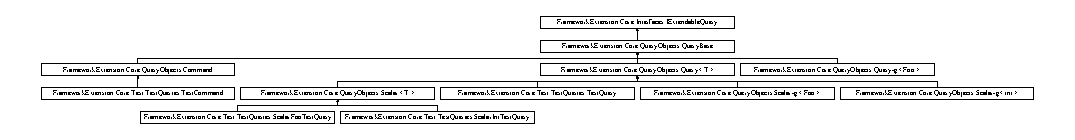
\includegraphics[height=1.435897cm]{class_framework_extension_1_1_core_1_1_query_objects_1_1_query_base}
\end{center}
\end{figure}
\subsection*{Public Member Functions}
\begin{DoxyCompactItemize}
\item 
\hypertarget{class_framework_extension_1_1_core_1_1_query_objects_1_1_query_base_ae3aea1df91af19d2d7a66d6fe4ec8298}{void {\bfseries Add\-Method\-Expression} (string method\-Name, Type\mbox{[}$\,$\mbox{]} generics, Expression\mbox{[}$\,$\mbox{]} parameters)}\label{class_framework_extension_1_1_core_1_1_query_objects_1_1_query_base_ae3aea1df91af19d2d7a66d6fe4ec8298}

\end{DoxyCompactItemize}
\subsection*{Protected Member Functions}
\begin{DoxyCompactItemize}
\item 
\hypertarget{class_framework_extension_1_1_core_1_1_query_objects_1_1_query_base_aaf9a0085a76601d6ee93ed18f4396661}{void {\bfseries Check\-Context\-And\-Query} (object query)}\label{class_framework_extension_1_1_core_1_1_query_objects_1_1_query_base_aaf9a0085a76601d6ee93ed18f4396661}

\end{DoxyCompactItemize}
\subsection*{Protected Attributes}
\begin{DoxyCompactItemize}
\item 
\hypertarget{class_framework_extension_1_1_core_1_1_query_objects_1_1_query_base_afe3fbbf0f6c22ff295b19a2eef649809}{List$<$ Tuple$<$ Method\-Info, \\*
Expression\mbox{[}$\,$\mbox{]}$>$ $>$ {\bfseries \-\_\-expression\-List} = new List$<$Tuple$<$Method\-Info, Expression\mbox{[}$\,$\mbox{]}$>$$>$()}\label{class_framework_extension_1_1_core_1_1_query_objects_1_1_query_base_afe3fbbf0f6c22ff295b19a2eef649809}

\end{DoxyCompactItemize}
\subsection*{Properties}
\begin{DoxyCompactItemize}
\item 
\hypertarget{class_framework_extension_1_1_core_1_1_query_objects_1_1_query_base_af50eb6f52cf3f0474c58181ccafe040a}{\hyperlink{interface_framework_extension_1_1_core_1_1_interfaces_1_1_i_data_context}{I\-Data\-Context} {\bfseries Context}\hspace{0.3cm}{\ttfamily  \mbox{[}get, set\mbox{]}}}\label{class_framework_extension_1_1_core_1_1_query_objects_1_1_query_base_af50eb6f52cf3f0474c58181ccafe040a}

\end{DoxyCompactItemize}
\subsection*{Events}
\begin{DoxyCompactItemize}
\item 
\hypertarget{class_framework_extension_1_1_core_1_1_query_objects_1_1_query_base_af88fe6bd4a96fd750d87b30c8a2a2b3a}{Event\-Handler$<$ \hyperlink{class_framework_extension_1_1_core_1_1_interceptors_1_1_events_1_1_pre_query_event_args}{Pre\-Query\-Event\-Args} $>$ {\bfseries Pre\-Query}}\label{class_framework_extension_1_1_core_1_1_query_objects_1_1_query_base_af88fe6bd4a96fd750d87b30c8a2a2b3a}

\item 
\hypertarget{class_framework_extension_1_1_core_1_1_query_objects_1_1_query_base_ad3ae4c0a5849c610d07492deb75097fd}{Event\-Handler$<$ \hyperlink{class_framework_extension_1_1_core_1_1_interceptors_1_1_events_1_1_post_query_event_args}{Post\-Query\-Event\-Args} $>$ {\bfseries Post\-Query}}\label{class_framework_extension_1_1_core_1_1_query_objects_1_1_query_base_ad3ae4c0a5849c610d07492deb75097fd}

\end{DoxyCompactItemize}


The documentation for this class was generated from the following file\-:\begin{DoxyCompactItemize}
\item 
Framework\-Extension.\-Core/\-Query\-Objects/Query\-Base.\-cs\end{DoxyCompactItemize}

\hypertarget{class_framework_extension_1_1_core_1_1_query_providers_1_1_query_translator-g}{\section{Framework\-Extension.\-Core.\-Query\-Providers.\-Query\-Translator$<$ T $>$ Class Template Reference}
\label{class_framework_extension_1_1_core_1_1_query_providers_1_1_query_translator-g}\index{Framework\-Extension.\-Core.\-Query\-Providers.\-Query\-Translator$<$ T $>$@{Framework\-Extension.\-Core.\-Query\-Providers.\-Query\-Translator$<$ T $>$}}
}
\subsection*{Public Member Functions}
\begin{DoxyCompactItemize}
\item 
\hypertarget{class_framework_extension_1_1_core_1_1_query_providers_1_1_query_translator-g_a0acb6be138aba15dd0495cdffdbe5326}{{\bfseries Query\-Translator} (I\-Queryable source)}\label{class_framework_extension_1_1_core_1_1_query_providers_1_1_query_translator-g_a0acb6be138aba15dd0495cdffdbe5326}

\item 
\hypertarget{class_framework_extension_1_1_core_1_1_query_providers_1_1_query_translator-g_a99babfddea0fe29b617975fc656ad25f}{{\bfseries Query\-Translator} (I\-Queryable source, Expression e)}\label{class_framework_extension_1_1_core_1_1_query_providers_1_1_query_translator-g_a99babfddea0fe29b617975fc656ad25f}

\item 
\hypertarget{class_framework_extension_1_1_core_1_1_query_providers_1_1_query_translator-g_a9a8d9e78cfaceca5581a0c2c60d91c3e}{I\-Enumerator$<$ T $>$ {\bfseries Get\-Enumerator} ()}\label{class_framework_extension_1_1_core_1_1_query_providers_1_1_query_translator-g_a9a8d9e78cfaceca5581a0c2c60d91c3e}

\item 
\hypertarget{class_framework_extension_1_1_core_1_1_query_providers_1_1_query_translator-g_a062155910b96326e40f32f2915b6f995}{Query\-Translator$<$ T $>$ {\bfseries Include} (String path)}\label{class_framework_extension_1_1_core_1_1_query_providers_1_1_query_translator-g_a062155910b96326e40f32f2915b6f995}

\end{DoxyCompactItemize}
\subsection*{Properties}
\begin{DoxyCompactItemize}
\item 
\hypertarget{class_framework_extension_1_1_core_1_1_query_providers_1_1_query_translator-g_a9174fe852650d95c0422f050fd9f7722}{Type {\bfseries Element\-Type}\hspace{0.3cm}{\ttfamily  \mbox{[}get\mbox{]}}}\label{class_framework_extension_1_1_core_1_1_query_providers_1_1_query_translator-g_a9174fe852650d95c0422f050fd9f7722}

\item 
\hypertarget{class_framework_extension_1_1_core_1_1_query_providers_1_1_query_translator-g_ac7f4d4c5d6eb0ecadebb0972ccddfe26}{Expression {\bfseries Expression}\hspace{0.3cm}{\ttfamily  \mbox{[}get\mbox{]}}}\label{class_framework_extension_1_1_core_1_1_query_providers_1_1_query_translator-g_ac7f4d4c5d6eb0ecadebb0972ccddfe26}

\item 
\hypertarget{class_framework_extension_1_1_core_1_1_query_providers_1_1_query_translator-g_a03460bcd4093d86d4937e1525af92666}{I\-Query\-Provider {\bfseries Provider}\hspace{0.3cm}{\ttfamily  \mbox{[}get\mbox{]}}}\label{class_framework_extension_1_1_core_1_1_query_providers_1_1_query_translator-g_a03460bcd4093d86d4937e1525af92666}

\end{DoxyCompactItemize}


The documentation for this class was generated from the following file\-:\begin{DoxyCompactItemize}
\item 
Framework\-Extension.\-Core/\-Query\-Providers/Query\-Provider.\-cs\end{DoxyCompactItemize}

\hypertarget{class_framework_extension_1_1_core_1_1_query_providers_1_1_query_translator_provider-g}{\section{Framework\-Extension.\-Core.\-Query\-Providers.\-Query\-Translator\-Provider$<$ T $>$ Class Template Reference}
\label{class_framework_extension_1_1_core_1_1_query_providers_1_1_query_translator_provider-g}\index{Framework\-Extension.\-Core.\-Query\-Providers.\-Query\-Translator\-Provider$<$ T $>$@{Framework\-Extension.\-Core.\-Query\-Providers.\-Query\-Translator\-Provider$<$ T $>$}}
}
\subsection*{Public Member Functions}
\begin{DoxyCompactItemize}
\item 
\hypertarget{class_framework_extension_1_1_core_1_1_query_providers_1_1_query_translator_provider-g_ab0c65223e0b5884df23f9ab7bb49d805}{{\bfseries Query\-Translator\-Provider} (I\-Queryable source)}\label{class_framework_extension_1_1_core_1_1_query_providers_1_1_query_translator_provider-g_ab0c65223e0b5884df23f9ab7bb49d805}

\item 
\hypertarget{class_framework_extension_1_1_core_1_1_query_providers_1_1_query_translator_provider-g_ae7c41665df72c69f32dcc82dd007bda3}{I\-Queryable$<$ T\-Element $>$ {\bfseries Create\-Query$<$ T\-Element $>$} (Expression expression)}\label{class_framework_extension_1_1_core_1_1_query_providers_1_1_query_translator_provider-g_ae7c41665df72c69f32dcc82dd007bda3}

\item 
\hypertarget{class_framework_extension_1_1_core_1_1_query_providers_1_1_query_translator_provider-g_ac1a76fcdabb96d88ceb4491a4a15e3b4}{I\-Queryable {\bfseries Create\-Query} (Expression expression)}\label{class_framework_extension_1_1_core_1_1_query_providers_1_1_query_translator_provider-g_ac1a76fcdabb96d88ceb4491a4a15e3b4}

\item 
\hypertarget{class_framework_extension_1_1_core_1_1_query_providers_1_1_query_translator_provider-g_ae24720331cd0aec88eafb055b01e6847}{T\-Result {\bfseries Execute$<$ T\-Result $>$} (Expression expression)}\label{class_framework_extension_1_1_core_1_1_query_providers_1_1_query_translator_provider-g_ae24720331cd0aec88eafb055b01e6847}

\item 
\hypertarget{class_framework_extension_1_1_core_1_1_query_providers_1_1_query_translator_provider-g_a9c6fcbe98906833d18b0ea173ec065e8}{object {\bfseries Execute} (Expression expression)}\label{class_framework_extension_1_1_core_1_1_query_providers_1_1_query_translator_provider-g_a9c6fcbe98906833d18b0ea173ec065e8}

\end{DoxyCompactItemize}
\subsection*{Protected Member Functions}
\begin{DoxyCompactItemize}
\item 
\hypertarget{class_framework_extension_1_1_core_1_1_query_providers_1_1_query_translator_provider-g_a76ceefe54562ff17e72d8ec01cc3e238}{override Expression {\bfseries Visit\-Constant} (Constant\-Expression c)}\label{class_framework_extension_1_1_core_1_1_query_providers_1_1_query_translator_provider-g_a76ceefe54562ff17e72d8ec01cc3e238}

\end{DoxyCompactItemize}


The documentation for this class was generated from the following file\-:\begin{DoxyCompactItemize}
\item 
Framework\-Extension.\-Core/\-Query\-Providers/Query\-Provider.\-cs\end{DoxyCompactItemize}

\hypertarget{class_framework_extension_1_1_core_1_1_query_objects_1_1_scalar-g}{\section{Framework\-Extension.\-Core.\-Query\-Objects.\-Scalar$<$ T $>$ Class Template Reference}
\label{class_framework_extension_1_1_core_1_1_query_objects_1_1_scalar-g}\index{Framework\-Extension.\-Core.\-Query\-Objects.\-Scalar$<$ T $>$@{Framework\-Extension.\-Core.\-Query\-Objects.\-Scalar$<$ T $>$}}
}
Inheritance diagram for Framework\-Extension.\-Core.\-Query\-Objects.\-Scalar$<$ T $>$\-:\begin{figure}[H]
\begin{center}
\leavevmode
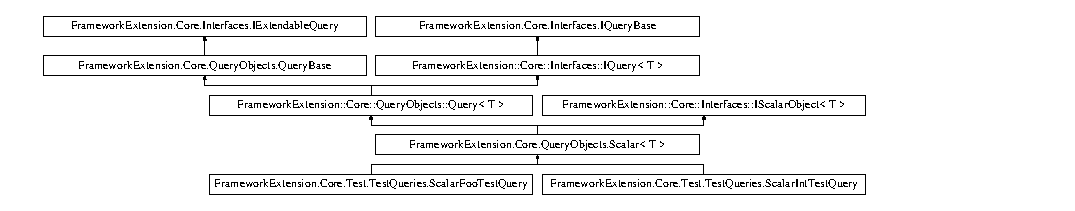
\includegraphics[height=2.393162cm]{class_framework_extension_1_1_core_1_1_query_objects_1_1_scalar-g}
\end{center}
\end{figure}
\subsection*{Public Member Functions}
\begin{DoxyCompactItemize}
\item 
\hypertarget{class_framework_extension_1_1_core_1_1_query_objects_1_1_scalar-g_ada3c86db2397c4c54e9fffed8ebe5891}{new T {\bfseries Execute} (\hyperlink{interface_framework_extension_1_1_core_1_1_interfaces_1_1_i_data_context}{I\-Data\-Context} context)}\label{class_framework_extension_1_1_core_1_1_query_objects_1_1_scalar-g_ada3c86db2397c4c54e9fffed8ebe5891}

\end{DoxyCompactItemize}
\subsection*{Properties}
\begin{DoxyCompactItemize}
\item 
Func$<$ \hyperlink{interface_framework_extension_1_1_core_1_1_interfaces_1_1_i_data_context}{I\-Data\-Context}, T $>$ \hyperlink{class_framework_extension_1_1_core_1_1_query_objects_1_1_scalar-g_ad6de4637a09a695d7934b52f5008369b}{Context\-Query}\hspace{0.3cm}{\ttfamily  \mbox{[}get, set\mbox{]}}
\begin{DoxyCompactList}\small\item\em This holds the expression that will be used to create the I\-Queryable
\begin{DoxyTemplParams}{Template Parameters}
{\em T} & \\
\hline
\end{DoxyTemplParams}
when executed on the context \end{DoxyCompactList}\end{DoxyCompactItemize}
\subsection*{Additional Inherited Members}


\subsection{Property Documentation}
\hypertarget{class_framework_extension_1_1_core_1_1_query_objects_1_1_scalar-g_ad6de4637a09a695d7934b52f5008369b}{\index{Framework\-Extension\-::\-Core\-::\-Query\-Objects\-::\-Scalar-\/g@{Framework\-Extension\-::\-Core\-::\-Query\-Objects\-::\-Scalar-\/g}!Context\-Query@{Context\-Query}}
\index{Context\-Query@{Context\-Query}!FrameworkExtension::Core::QueryObjects::Scalar-g@{Framework\-Extension\-::\-Core\-::\-Query\-Objects\-::\-Scalar-\/g}}
\subsubsection[{Context\-Query}]{\setlength{\rightskip}{0pt plus 5cm}template$<$T $>$ Func$<${\bf I\-Data\-Context}, T$>$ {\bf Framework\-Extension.\-Core.\-Query\-Objects.\-Scalar}$<$ T $>$.Context\-Query\hspace{0.3cm}{\ttfamily [get]}, {\ttfamily [set]}}}\label{class_framework_extension_1_1_core_1_1_query_objects_1_1_scalar-g_ad6de4637a09a695d7934b52f5008369b}


This holds the expression that will be used to create the I\-Queryable
\begin{DoxyTemplParams}{Template Parameters}
{\em T} & \\
\hline
\end{DoxyTemplParams}
when executed on the context 



Reimplemented from \hyperlink{class_framework_extension_1_1_core_1_1_query_objects_1_1_query-g_afc262d00f1a554c09fe74d2079d5e4c7}{Framework\-Extension.\-Core.\-Query\-Objects.\-Query$<$ T $>$}.



The documentation for this class was generated from the following file\-:\begin{DoxyCompactItemize}
\item 
Framework\-Extension.\-Core/\-Query\-Objects/Scalar.\-cs\end{DoxyCompactItemize}

\hypertarget{class_framework_extension_1_1_core_1_1_test_1_1_test_queries_1_1_scalar_foo_test_query}{\section{Framework\-Extension.\-Core.\-Test.\-Test\-Queries.\-Scalar\-Foo\-Test\-Query Class Reference}
\label{class_framework_extension_1_1_core_1_1_test_1_1_test_queries_1_1_scalar_foo_test_query}\index{Framework\-Extension.\-Core.\-Test.\-Test\-Queries.\-Scalar\-Foo\-Test\-Query@{Framework\-Extension.\-Core.\-Test.\-Test\-Queries.\-Scalar\-Foo\-Test\-Query}}
}
Inheritance diagram for Framework\-Extension.\-Core.\-Test.\-Test\-Queries.\-Scalar\-Foo\-Test\-Query\-:\begin{figure}[H]
\begin{center}
\leavevmode
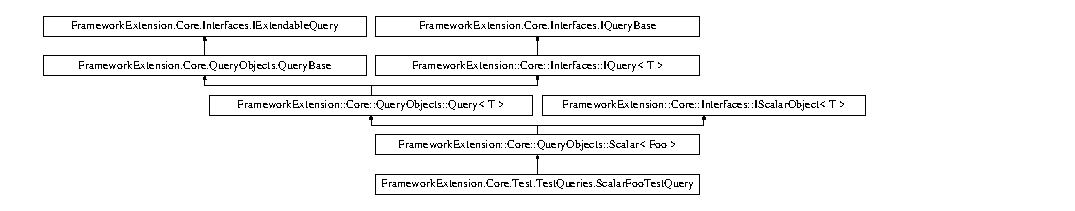
\includegraphics[height=2.393162cm]{class_framework_extension_1_1_core_1_1_test_1_1_test_queries_1_1_scalar_foo_test_query}
\end{center}
\end{figure}
\subsection*{Additional Inherited Members}


The documentation for this class was generated from the following file\-:\begin{DoxyCompactItemize}
\item 
Framework\-Extension.\-Core.\-Test/\-Test\-Queries/Scalar\-Foo\-Test\-Query.\-cs\end{DoxyCompactItemize}

\hypertarget{class_framework_extension_1_1_core_1_1_test_1_1_test_queries_1_1_scalar_int_test_query}{\section{Framework\-Extension.\-Core.\-Test.\-Test\-Queries.\-Scalar\-Int\-Test\-Query Class Reference}
\label{class_framework_extension_1_1_core_1_1_test_1_1_test_queries_1_1_scalar_int_test_query}\index{Framework\-Extension.\-Core.\-Test.\-Test\-Queries.\-Scalar\-Int\-Test\-Query@{Framework\-Extension.\-Core.\-Test.\-Test\-Queries.\-Scalar\-Int\-Test\-Query}}
}
Inheritance diagram for Framework\-Extension.\-Core.\-Test.\-Test\-Queries.\-Scalar\-Int\-Test\-Query\-:\begin{figure}[H]
\begin{center}
\leavevmode
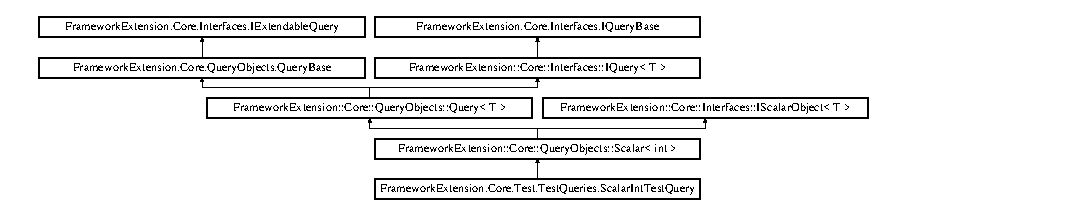
\includegraphics[height=2.449694cm]{class_framework_extension_1_1_core_1_1_test_1_1_test_queries_1_1_scalar_int_test_query}
\end{center}
\end{figure}
\subsection*{Additional Inherited Members}


The documentation for this class was generated from the following file\-:\begin{DoxyCompactItemize}
\item 
Framework\-Extension.\-Core.\-Test/\-Test\-Queries/Scalar\-Int\-Test\-Query.\-cs\end{DoxyCompactItemize}

\hypertarget{class_framework_extension_1_1_core_1_1_test_1_1_test_queries_1_1_test_command}{\section{Framework\-Extension.\-Core.\-Test.\-Test\-Queries.\-Test\-Command Class Reference}
\label{class_framework_extension_1_1_core_1_1_test_1_1_test_queries_1_1_test_command}\index{Framework\-Extension.\-Core.\-Test.\-Test\-Queries.\-Test\-Command@{Framework\-Extension.\-Core.\-Test.\-Test\-Queries.\-Test\-Command}}
}
Inheritance diagram for Framework\-Extension.\-Core.\-Test.\-Test\-Queries.\-Test\-Command\-:\begin{figure}[H]
\begin{center}
\leavevmode
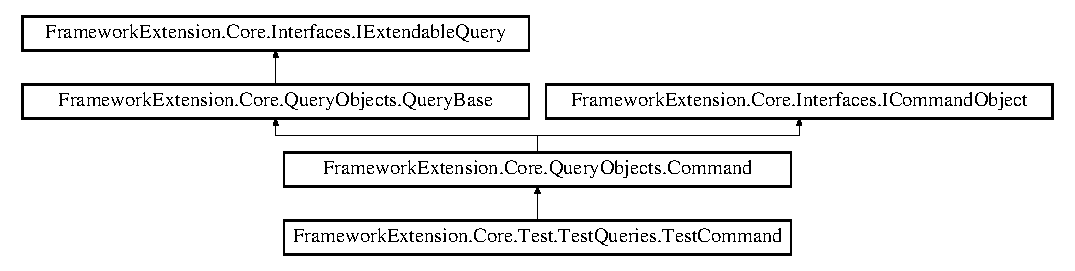
\includegraphics[height=3.200000cm]{class_framework_extension_1_1_core_1_1_test_1_1_test_queries_1_1_test_command}
\end{center}
\end{figure}
\subsection*{Properties}
\begin{DoxyCompactItemize}
\item 
\hypertarget{class_framework_extension_1_1_core_1_1_test_1_1_test_queries_1_1_test_command_aeb5c699821557093271e2a1184bd390a}{bool {\bfseries Called}\hspace{0.3cm}{\ttfamily  \mbox{[}get, set\mbox{]}}}\label{class_framework_extension_1_1_core_1_1_test_1_1_test_queries_1_1_test_command_aeb5c699821557093271e2a1184bd390a}

\end{DoxyCompactItemize}
\subsection*{Additional Inherited Members}


The documentation for this class was generated from the following file\-:\begin{DoxyCompactItemize}
\item 
Framework\-Extension.\-Core.\-Test/\-Test\-Queries/Test\-Command.\-cs\end{DoxyCompactItemize}

\hypertarget{class_framework_extension_1_1_entity_framework_1_1_tests_1_1_mapping_1_1_test_mapping_configuration}{\section{Framework\-Extension.\-Entity\-Framework.\-Tests.\-Mapping.\-Test\-Mapping\-Configuration Class Reference}
\label{class_framework_extension_1_1_entity_framework_1_1_tests_1_1_mapping_1_1_test_mapping_configuration}\index{Framework\-Extension.\-Entity\-Framework.\-Tests.\-Mapping.\-Test\-Mapping\-Configuration@{Framework\-Extension.\-Entity\-Framework.\-Tests.\-Mapping.\-Test\-Mapping\-Configuration}}
}
Inheritance diagram for Framework\-Extension.\-Entity\-Framework.\-Tests.\-Mapping.\-Test\-Mapping\-Configuration\-:\begin{figure}[H]
\begin{center}
\leavevmode
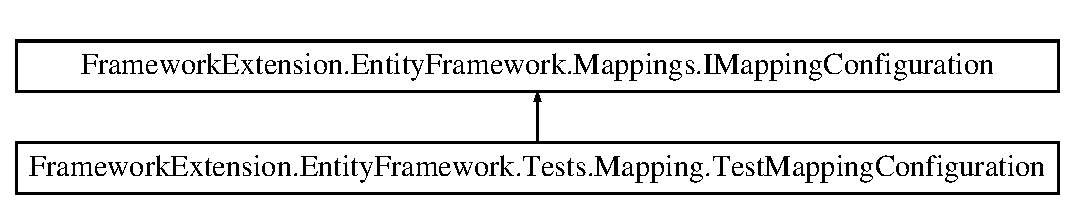
\includegraphics[height=2.000000cm]{class_framework_extension_1_1_entity_framework_1_1_tests_1_1_mapping_1_1_test_mapping_configuration}
\end{center}
\end{figure}
\subsection*{Public Member Functions}
\begin{DoxyCompactItemize}
\item 
void \hyperlink{class_framework_extension_1_1_entity_framework_1_1_tests_1_1_mapping_1_1_test_mapping_configuration_ab3e0ed1691f37fa30871356ba49f88eb}{Configure\-Model\-Builder} (Db\-Model\-Builder model\-Builder)
\begin{DoxyCompactList}\small\item\em This method takes the model\-Builder from Entity Framework and wires in the mappings provided \end{DoxyCompactList}\end{DoxyCompactItemize}


\subsection{Member Function Documentation}
\hypertarget{class_framework_extension_1_1_entity_framework_1_1_tests_1_1_mapping_1_1_test_mapping_configuration_ab3e0ed1691f37fa30871356ba49f88eb}{\index{Framework\-Extension\-::\-Entity\-Framework\-::\-Tests\-::\-Mapping\-::\-Test\-Mapping\-Configuration@{Framework\-Extension\-::\-Entity\-Framework\-::\-Tests\-::\-Mapping\-::\-Test\-Mapping\-Configuration}!Configure\-Model\-Builder@{Configure\-Model\-Builder}}
\index{Configure\-Model\-Builder@{Configure\-Model\-Builder}!FrameworkExtension::EntityFramework::Tests::Mapping::TestMappingConfiguration@{Framework\-Extension\-::\-Entity\-Framework\-::\-Tests\-::\-Mapping\-::\-Test\-Mapping\-Configuration}}
\subsubsection[{Configure\-Model\-Builder}]{\setlength{\rightskip}{0pt plus 5cm}void Framework\-Extension.\-Entity\-Framework.\-Tests.\-Mapping.\-Test\-Mapping\-Configuration.\-Configure\-Model\-Builder (
\begin{DoxyParamCaption}
\item[{Db\-Model\-Builder}]{model\-Builder}
\end{DoxyParamCaption}
)\hspace{0.3cm}{\ttfamily [inline]}}}\label{class_framework_extension_1_1_entity_framework_1_1_tests_1_1_mapping_1_1_test_mapping_configuration_ab3e0ed1691f37fa30871356ba49f88eb}


This method takes the model\-Builder from Entity Framework and wires in the mappings provided 


\begin{DoxyParams}{Parameters}
{\em model\-Builder} & The Database model builder used by Entity Framework to generate the model.\\
\hline
\end{DoxyParams}


Implements \hyperlink{interface_framework_extension_1_1_entity_framework_1_1_mappings_1_1_i_mapping_configuration_a4c3e96e66c2a5c926b2cf6d60d7289a6}{Framework\-Extension.\-Entity\-Framework.\-Mappings.\-I\-Mapping\-Configuration}.



The documentation for this class was generated from the following file\-:\begin{DoxyCompactItemize}
\item 
Framework\-Extension.\-Entity\-Framework.\-Tests/\-Mapping/Test\-Mapping\-Configuration.\-cs\end{DoxyCompactItemize}

\hypertarget{class_framework_extension_1_1_core_1_1_test_1_1_test_queries_1_1_test_query}{\section{Framework\-Extension.\-Core.\-Test.\-Test\-Queries.\-Test\-Query Class Reference}
\label{class_framework_extension_1_1_core_1_1_test_1_1_test_queries_1_1_test_query}\index{Framework\-Extension.\-Core.\-Test.\-Test\-Queries.\-Test\-Query@{Framework\-Extension.\-Core.\-Test.\-Test\-Queries.\-Test\-Query}}
}
Inheritance diagram for Framework\-Extension.\-Core.\-Test.\-Test\-Queries.\-Test\-Query\-:\begin{figure}[H]
\begin{center}
\leavevmode
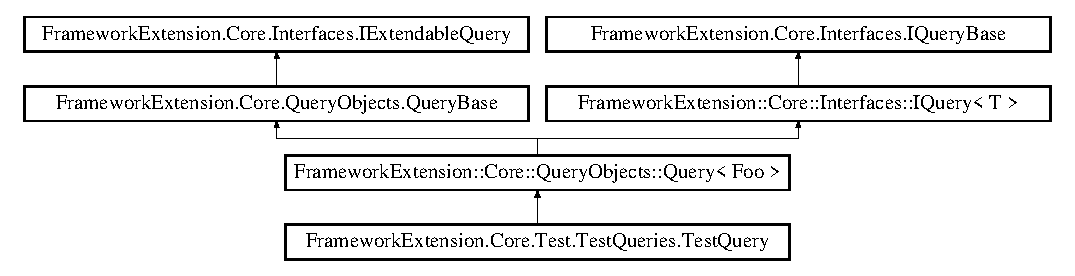
\includegraphics[height=3.255814cm]{class_framework_extension_1_1_core_1_1_test_1_1_test_queries_1_1_test_query}
\end{center}
\end{figure}
\subsection*{Additional Inherited Members}


The documentation for this class was generated from the following file\-:\begin{DoxyCompactItemize}
\item 
Framework\-Extension.\-Core.\-Test/\-Test\-Queries/Test\-Query.\-cs\end{DoxyCompactItemize}

\printindex
\end{document}
